\documentclass[10pt, oneside]{article}
\usepackage{amsmath, amsthm, amssymb, calrsfs, wasysym, verbatim, bbm, hyperref}
\usepackage{graphicx}
\usepackage{wasysym}
\usepackage{float}
\usepackage{mathrsfs}
\usepackage{graphicx}
\usepackage{subcaption}
\usepackage{algorithm}
\usepackage{algpseudocode}
\usepackage{mathrsfs}
\usepackage{statistics-note-style}
\newcommand{\todo}{\textcolor{pink}{TODO}}


\newcommand{\indep}{\perp\!\!\!\perp}
\newcommand{\dd}{\mathop{}\!\mathrm{d}}
\newcommand{\EE}{\mathbb{E}}
\newcommand{\RR}{\mathbb{R}}
\newcommand{\HH}{\mathbb{H}}
\newcommand{\CC}{\mathbb{C}}
\newcommand{\ZZ}{\mathbb{Z}}
\newcommand{\NN}{\mathbb{N}}
\newcommand{\PP}{\mathbb{P}}
\newcommand{\QQ}{\mathbb{Q}}
\newcommand{\cF}{\mathcal{F}}
\newcommand{\cN}{\mathcal{N}}
\newcommand{\cM}{\mathcal{M}}
\newcommand{\cX}{\mathcal{X}}
\newcommand{\Cdot}{\boldsymbol{\cdot}}
\newcommand{\simiid}{\overset{\text{i.i.d.}}{\sim}}
\newcommand{\tod}{\overset{\text{d}}{\to}}
\newcommand{\normalg}{\mathcal{N}(0,1)}
\newcommand{\tr}{\operatorname{tr}}
\newcommand{\diag}{\operatorname{diag}}
\newcommand{\Id}{\operatorname{Id}}
\newcommand{\Cat}{\operatorname{Cat}}
\newcommand{\Poi}{\operatorname{Poi}}
\newcommand{\Var}{\operatorname{Var}}
\newcommand{\mc}{\mathcal}
\newcommand{\e}{\mathrm{e}}
\newcommand{\ii}{\mathrm{i}}
\newcommand{\sgn}{\operatorname{sgn}}
\newcommand{\softmax}{\operatorname{Softmax}}
\newcommand{\bx}{\mathbf{x}}
\newcommand{\bX}{\mathbf{X}}
\newcommand{\bY}{\mathbf{Y}}
\newcommand{\bI}{\mathbf{I}}
\newcommand{\bV}{\mathbf{V}}
\newcommand{\bv}{\mathbf{v}}
\newcommand{\bbeta}{\mathbf{\beta}}
\newcommand{\hbbeta}{\hat{\mathbf{\beta}}}
\newcommand{\bvarepsilon}{\mathbf{\varepsilon}}
\newcommand{\bzero}{\mathbf{0}}
\newcommand{\bSigma}{\mathbf{\Sigma}}
\newcommand{\cH}{\mathcal{H}}
\newcommand{\cT}{\mathcal{T}}


\newtheoremstyle{notestyle}%
  {7pt}{7pt}{\normalfont}{}%
  {\sffamily\bfseries\color{Ink}}{.}{0.55em}{}%
\theoremstyle{notestyle}
\newtheorem{thm}{Theorem}[section] 
\newtheorem{defn}[thm]{Definition} 
\newtheorem{conv}[thm]{Convention} 
\newtheorem{rem}[thm]{Remark}      
\newtheorem{lem}[thm]{Lemma}       
\newtheorem{cor}[thm]{Corollary}   
\newtheorem{prop}[thm]{Proposition}
\newtheorem{exam}[thm]{Example}
\newtheorem{appr}[thm]{Approach}
\newtheorem{obs}[thm]{Observation}


\title{A Guided Tour of Modern Statistics}
\author{Zixun Huang}
\begin{document}

\maketitle
\tableofcontents

\vspace{.25in}

\newpage
\part{Chapter 1: Classical Theory}
\newpage
\section{Probability Theory and Stochastic Processes}
In this chapter, we introduce the basic notation and fundamental tools of probability theory and measure theory that will be used throughout the subsequent chapters. The section is organized as follows: 
\begin{enumerate}
    \item probability space and random variables;
    \item modes of convergence;
    \item the Law of Large Numbers (LLN) and the Central Limit Theorem (CLT);
    \item martingales, Markov chains and Brownian motion. 
\end{enumerate}

This section mainly follows Introduction to Probability Theory (Tsinghua University), Stochastic Processes (Peking University), Stochastic Analysis (Peking University), Math C218A (UC Berkeley), Math C218B (UC Berkeley) and the book Probability: Theory and Examples by Rick Durrett~\cite{durrett2019probability}, Sinho Chewi's notes of MATH C218A, and Introduction to Stochastic Processes~\cite{lawler2018introduction}.

\subsection{Probability Space and Random Variables}
\subsubsection{Probability space}
A probability space \( (\Omega, \mathcal{F}, P) \) contains three elements:
\begin{itemize}
    \item The space \(\Omega\): this is a non-empty set. It can be viewed as the set of all possible outcomes.
    \item The \(\sigma\)-field \(\mathcal{F}\): this can be viewed as a collection of all the events.
    \item The probability measure \(P\): this is a function from \(\mathcal{F}\) to \([0, 1]\). It gives a probability to each event.
\end{itemize}

\begin{defn}[$\sigma-$Field]
    Suppose \(\mathcal{F}\) is a non-empty collection of subsets of \(\Omega\).
    \begin{itemize}
        \item It is a field if it is closed under \textbf{complementation} and closed under \textbf{union}:
        \[
        A \in \mathcal{F} \implies A^c \in \mathcal{F}, \quad A_1, A_2 \in \mathcal{F} \implies A_1 \cup A_2 \in \mathcal{F}.
        \]
        \item It is a \textbf{monotone class} if
        \[
        A_j \in \mathcal{F}, \, A_j \subset A_{j+1}, \, 1 \leq j < \infty \implies \bigcup_j A_j \in \mathcal{F},
        \]
        and
        \[
        A_j \in \mathcal{F}, \, A_j \supset A_{j+1}, \, 1 \leq j < \infty \implies \bigcap_j A_j \in \mathcal{F}.
        \]
        \item It is a \(\sigma\)-field if it is closed under \textbf{complementation} and closed under \textbf{countable union}:
        \[
        A \in \mathcal{F} \implies A^c \in \mathcal{F}, \quad A_j \in \mathcal{F}, \, 1 \leq j < \infty \implies \bigcup_j A_j \in \mathcal{F}.
        \]
    \end{itemize}
\end{defn}

\begin{defn}[Generated $\sigma$-Fields]
Given any collection \( C \) of sets, the \(\sigma\)-field generated by \( C \) is the intersection of all \(\sigma\)-fields containing \( C \).
\end{defn}

\begin{defn}[Probability Measure]
    Suppose \(\mathcal{F}\) is a \(\sigma\)-field on \(\Omega\). A probability measure \(P\) is a function from \(\mathcal{F}\) to \([0, 1]\) satisfying the following axioms:
    \begin{itemize}
        \item \(P[E] \geq 0\) for all \(E \in \mathcal{F}\);
        \item \(P[\Omega] = 1\);
        \item If \(\{E_j\}_{j}\) is a countable collection of pairwise disjoint sets in \(\mathcal{F}\), then:
        \[
        P\left[\bigcup_j E_j\right] = \sum_j P[E_j].
        \]
    \end{itemize}
    These axioms imply the following consequences:
    \begin{itemize}
        \item \(P[E^c] = 1 - P[E]\);
        \item \(P[E \cup F] + P[E \cap F] = P[E] + P[F]\);
        \item Continuity: if \(E_n \uparrow E\) or \(E_n \downarrow E\), then \(P[E_n] \to P[E]\);
        \item \(P\left[\bigcup_j E_j\right] \leq \sum_j P[E_j]\).
    \end{itemize}
\end{defn}

\begin{rem}
    We care about the $\sigma$-field because that is where our random variables live. It defines the rules under which stochastic analysis can work. Sometimes we need to enlarge our space to a bigger $\sigma$-field and make sure the measure still fits — this is guaranteed by the following theorem.
\end{rem}


\begin{thm}[Carathéodory’s Extension Theorem]
    Suppose \(\mathcal{F}_0\) is a field and \(\mathcal{F}\) is the \(\sigma\)-field generated by \(\mathcal{F}_0\). Suppose \(\mu\) is a probability measure on \(\mathcal{F}_0\). Then there exists a unique probability measure on \(\mathcal{F}\) that coincides with \(\mu\) on \(\mathcal{F}_0\).
\end{thm}

\begin{rem}
    The construction: 
    \[
    \tau(A)=\inf\left\{
    \sum_{n=1}^\infty \mu(B_n): B_n\in \mathcal{F}, \ A\subset\bigcup_{n=1}^\infty B_n
    \right\}.
    \]
\end{rem}



\subsubsection{Random Variables}
\begin{defn}[Random Variables]
    A real-valued random variable is a function \( X: \Omega \to \mathbb{R} \) such that
    \[
    X^{-1}(B) \in \mathcal{F}, \quad \forall B \in \mathcal{B}.
    \]
    In other words, a random variable is just a \textbf{measurable} function from \( (\Omega, \mathcal{F}) \) to \( (\mathbb{R}, \mathcal{B}) \).
\end{defn}
\begin{defn}[Distribution]
    Each random variable \( X \) induces a probability measure \( \mu \) on \( (\mathbb{R}, \mathcal{B}) \) by the following correspondence:
    \[
    \mu[B] = P[X^{-1}(B)] = P[X \in B], \quad \forall B \in \mathcal{B}.
    \]
    The measure \( \mu \) is called the law (or the distribution) of \( X \), denoted by \( \mathcal{L}(X) \); its associated distribution function is called the distribution function of \( X \), denoted by \( F_X \).
\end{defn}
The concept of ``expectation'' is the same as integration in the probability space \( (\Omega, \mathcal{F}, \mathbb{P}) \).
\begin{cor}
    If \( X \) takes only positive integer values, we have
    \[
    \mathbb{E}[X] = \sum_{n=1}^{\infty} \mathbb{P}[X \geq n].
    \]
\end{cor}

\begin{defn}[$p$-th Moment]
    For any \( p \in (0, \infty) \), define
    \[
    L^p(\Omega, \mathcal{F}, \mathbb{P}) = \left\{ X \text{ random variable on } (\Omega, \mathcal{F}, \mathbb{P}) : \mathbb{E}[|X|^p] < \infty \right\}.
    \]
    For \( X \in L^p \), we call \( \mathbb{E}[|X|^p] \) the \( p \)-th moment of \( X \).
\end{defn}

\begin{defn}[Independent]
    The random variables \( \{ X_j, 1 \leq j \leq n \} \) are independent if, for any Borel sets \( \{ B_j, 1 \leq j \leq n \} \), we have
    \[
    \mathbb{P}\left[\bigcap_{j=1}^n \{ X_j \in B_j \}\right] = \prod_{j=1}^n \mathbb{P}[X_j \in B_j].
    \]
    The random variables \( \{ X_j, j \geq 1 \} \) are independent if \( \{ X_j, 1 \leq j \leq n \} \) are independent for all \( n \).
\end{defn}

\begin{thm}
    Suppose \( \{ A_j, 1 \leq j \leq n \} \) are independent and each \( A_j \) is a \(\pi\)-system. Denote by \( \sigma(A_j) \) the \(\sigma\)-field generated by \( A_j \) for each \( j \). Then \( \{ \sigma(A_j), 1 \leq j \leq n \} \) are independent.
\end{thm}

\begin{exam}[Kolmogorov’s 0-1 Law]
    Let \( \{ X_n \} \) be a sequence of independent random variables. Let
    \[
    G_n = \sigma(X_k, k \geq n) \quad \text{and} \quad G_\infty = \bigcap_{n \geq 1} G_n.
    \]
    Then \( G_\infty \) is trivial, i.e., for any \( A \in G_\infty \), we have
    \[
    \mathbb{P}[A] = 0 \text{ or } 1.
    \]
    Define \( S_n = \sum_{j=1}^{n} X_j \). It is clear that the following events are in \( G_\infty \):
    \[
    \lim_{n \to \infty} S_n \text{ exists}, \quad \lim_{n \to \infty} \frac{S_n}{n} \text{ exists}, \quad \limsup_{n \to \infty} \frac{S_n}{n} > 0.
    \]
    Whereas, the following event is not in \( G_\infty \):
    \[
    \limsup_{n \to \infty} S_n > 0.
    \]
\end{exam}

\begin{proof}
    On the one hand, we have \( A \in G_{n+1} \) for any \( n \). Thus, \( A \) is independent of \( \sigma(X_1, \dots, X_n) \) for any \( n \). Therefore, \( A \) is independent of \( \sigma(X_n, n \geq 1) \). On the other hand, \( A \) is measurable with respect to \( \sigma(X_n, n \geq 1) \). Therefore, \( A \) is independent of itself. This implies \( \mathbb{P}[A] = \mathbb{P}[A \cap A] = \mathbb{P}[A]^2 \), thus \( \mathbb{P}[A] \in \{ 0, 1 \} \).
\end{proof}

Now let's talk about Gaussians. The key thing to know is that Gaussians stay Gaussian under linear combinations and projections.
\begin{prop}
   The following are equivalent:
    \begin{enumerate}
        \item The random vector \( \xi = (\xi_1, \dots, \xi_d)^\top \) follows a \( d \)-dimensional Gaussian distribution.
        \item For any \( a_1, \dots, a_d \), the linear combination \( \sum_{k=1}^d a_k \xi_k \) follows a one-dimensional Gaussian distribution.
    \end{enumerate} 
\end{prop}


\subsection{Convergence}
\subsubsection{Convergence: Almost Sure, in Probability, and in \texorpdfstring{$L^p$}{Lp}}
\begin{defn}[Almost sure convergence (a.s.))]
    The sequence of random variables \( \{ X_n \} \) converges a.s. to the random variable \( X \) if there exists a null set \( \mathcal{N} \) such that
    \[
    \lim_{n \to \infty} X_n(\omega) = X(\omega), \quad \forall \omega \in \Omega \setminus \mathcal{N}.
    \]
\end{defn}

\begin{defn}[Convergence in probability] 
    The sequence \( \{ X_n \} \) converges in probability to the random variable \( X \) if, for every \( \epsilon > 0 \), we have
    \[
    \lim_{n \to \infty} \mathbb{P}[|X_n - X| > \epsilon] = 0.
    \]
\end{defn}

\begin{defn}[Convergence in \( L^p \))] 
    Assume \( p \geq 1 \). The sequence \( \{ X_n \} \) converges in \( L^p \) to the random variable \( X \) if \( X_n \in L^p \), \( X \in L^p \) and
    \[
    \lim_{n \to \infty} \mathbb{E}[|X_n - X|^p] = 0.
    \]
\end{defn}

It is straightforward to prove that almost sure convergence (\(a.s.\)) implies convergence in probability, and convergence in \(L^p\) implies convergence in probability. However, almost sure convergence (\(a.s.\)) and \(L^p\) may not imply each other. Now we talk about an example: using probability methods to prove Weierstrass Theorem.

\begin{exam}[Weierstrass Theorem]
    Let \( f \) be a continuous function on \( [0, 1] \). Define the polynomial:
\[
f_n(x) = \sum_{j=0}^{n} \binom{n}{j} x^j (1 - x)^{n - j} f\left( \frac{j}{n} \right).
\]
This is called the Bernstein polynomial of degree \( n \) associated to \( f \). Then we have
\[
\sup_{x \in [0, 1]} |f_n(x) - f(x)| \to 0, \quad n \to \infty.
\]
\end{exam}

\begin{proof}
    Suppose \( \{ X_j, j \geq 1 \} \) are i.i.d. Bernoulli variables with parameter \( p \in [0, 1] \): \( \mathbb{P}[X_j = 1] = p, \mathbb{P}[X_j = 0] = 1 - p \), and set \( S_n = \sum_{j=1}^{n} X_j \). Then we find
\[
\mathbb{E}[X_j] = p, \quad \text{var}(X_j) = p(1 - p), \quad \mathbb{E}[S_n] = np, \quad \text{var}(S_n) = np(1 - p).
\]
Moreover, 
\[
\mathbb{P}[S_n = j] = \binom{n}{j} p^j (1 - p)^{n - j}, \quad \text{thus} \quad f_n(p) = \mathbb{E}[f(S_n/n)].
\]
Note that \( f \) is bounded: \( |f| \leq M \), and it is uniformly continuous: for any \( \epsilon > 0 \), there exists \( \delta > 0 \) such that \( |f(x) - f(y)| \leq \epsilon \) as long as \( |x - y| \leq \delta \). Thus,
\[
|f_n(p) - f(p)| \leq \mathbb{E}[|f(S_n/n) - f(p)|] \leq \epsilon + 2M \mathbb{P}[|S_n/n - p| > \delta].
\]
Note that
\[
\mathbb{P}[|S_n/n - p| > \delta] \leq \frac{\text{var}(S_n)}{n^2 \delta^2} = \frac{p(1 - p)}{n \delta^2} \leq \frac{1}{4n \delta^2}.
\]
Thus,
\[
|f_n(p) - f(p)| \leq \epsilon + \frac{M}{2n \delta^2}.
\]
\end{proof}

We give a useful lemma to prove almost surely convergence.
\begin{thm}[Borel-Cantelli Lemma]
\label{BC_lemma}
\begin{itemize}
    \item For arbitrary sequence \( \{ E_n \} \), we have
    \[
    \sum_n \mathbb{P}[E_n] < \infty \quad \Rightarrow \quad \mathbb{P}[E_n \text{ i.o.}] = 0.
    \]
    \item If the events \( \{ E_n \} \) are independent, we have
    \[
    \sum_n \mathbb{P}[E_n] = \infty \quad \Rightarrow \quad \mathbb{P}[E_n \text{ i.o.}] = 1.
    \]
\end{itemize}
\end{thm}

\subsubsection{Weak Convergence}
\begin{defn}[Weak Convergence]
    A sequence of measures \( \{ \mu_n \} \) converges weakly to a measure \( \mu \) if
    \[
    \mu_n((a, b]) \to \mu((a, b]), \quad \text{for all continuity points} \ a, b \ \text{of} \ \mu.
    \]
    We denote by \( \mu_n \Rightarrow \mu \).
\end{defn}

\begin{prop}
    Suppose \( \{ \mu_n \} \) and \( \mu \) are probability measures. Then \( \mu_n \Rightarrow \mu \) if and only if
\[
\lim_{n \to \infty} \int f(x) \, \mu_n[d x] \to \int f(x) \, \mu[d x], \quad \forall f \in C_b:=\text{(bounded continuous functions)}.
\]
\end{prop}

\subsubsection{Convergence in Distribution}
\begin{defn}[Convergence in Distribution]
    A sequence of random variables \( \{ X_n \} \) converges in distribution to a random variable \( X \) if distribution function \( \mathcal{L}(X_n) \Rightarrow \mathcal{L}(X) \). We denote by \( X_n \xrightarrow{d} X \), or \( X_n \to X \) in distribution.
\end{defn}
Convergence in probability implies convergence in distribution. Furthermore, convergence in distribution is equivalent to the convergence of \textbf{characteristic functions}.

\begin{defn}[Characteristic Function]
For any random variable $X$ with distribution $\mu$, its characteristic function is defined to be:
\[
f: \mathbb{R} \to \mathbb{C}, \quad f(t) := \mathbb{E}\left[e^{itX}\right] = \int e^{itx} \, \mu[dx].
\]
\end{defn}

The distribution is uniquely identified by the characteristic function.
\begin{thm}
Suppose $f$ is the characteristic function for the probability measure $\mu$. For $x < y$, we have
\[
\mu[(x, y)] + \frac{1}{2}\mu[\{x\}] + \frac{1}{2}\mu[\{y\}] = \lim_{T \to \infty} \frac{1}{2\pi} \int_{-T}^{T} \frac{e^{-itx} - e^{-ity}}{it} f(t) \, dt.
\]
\end{thm}

\begin{thm}
Let $\{\mu_n\}$ be a sequence of probability measures with characteristic functions $\{f_n\}$. Suppose that
\begin{enumerate}
    \item $f_n$ converges everywhere in $\mathbb{R}$ and defines the limiting function $f$;
    \item $f$ is continuous at $t = 0$.
\end{enumerate}
Then we have
\begin{enumerate}
    \item $\mu_n \xrightarrow{d} \mu$ where $\mu$ is a probability measure;
    \item the characteristic function of $\mu$ is $f$.
\end{enumerate}
\end{thm}

At the end of this subsection, we introduce some useful convergence results. Let \( (X_n) \) be a sequence of random variables and let \( X \) be a random variable such that \( X_n \to X \) (a.s.):
\[
\mathbb{P}(X_n \to X) = 1.
\]

We state the convergence properties as follows:

\begin{itemize}
    \item \textbf{(MON)} If \( 0 \leq X_n \uparrow X \), then \( \mathbb{E}(X_n) \leq \mathbb{E}(X) < \infty \);
    \item \textbf{(FATOU)} If \( X_n \geq 0 \), then \( \mathbb{E}(X_n) \leq \liminf \mathbb{E}(X_n) \);
    \item \textbf{(DOM)} If \( |X_n(\omega)| \leq Y(\omega), \, \forall (n, \omega), \text{ and } \mathbb{E}(Y) < \infty \), then
    \[
    \mathbb{E}(|X_n - X|) \to 0,
    \]
    \item \textbf{(SCHEFFÉ)} If \( \mathbb{E}(|X_n|) \to \mathbb{E}(|X|) \), then
    \[
    \mathbb{E}(|X_n - X|) \to 0;
    \]
    \item \textbf{(BDD)} If there exists a constant \( K \), such that \( |X_n(\omega)| \leq K, \, \forall (n, \omega) \), then
    \[
    \mathbb{E}(|X_n - X|) \to 0.
    \]
\end{itemize}


\subsection{The Law of Large Numbers and the Central Limit Theorem}
\subsubsection{Strong Law of Large Numbers}
We will give three versions (4th moment SLLN, 2nd moment SLLN and SLLN).
\begin{thm}[4th Moment SLLN]
Let $(X_i, 1 \leq i < \infty)$ be IID, $EX = 0$, and $EX^4 < \infty$. Write $S_n = \sum_{i=1}^{n} X_i$. Then
\begin{enumerate}
    \item $ES_n^4 \leq 3n^2 EX^4$
    \item $S_n/n \to 0$ as $n \to \infty$.
\end{enumerate}
\end{thm}

If $EX = \mu$, applying the theorem to $X - \mu$ shows that $S_n/n \to \mu$ a.s.

\begin{proof}
    \begin{align*}
    ES_n^4 &=\sum_i \sum_j \sum_k \sum_l E[X_i X_j X_k X_l]\\
    &= nEX^4 + \binom{4}{2}\binom{n}{2} E[X_1^2 X_2^2] \\
    &= nEX^4 + 3n(n-1) \underbrace{(EX^2)^2}_{\leq EX^4}
    \end{align*}
    since $(EY)^2 \leq E(Y^2)$.
 Fix $\varepsilon > 0$.
    \begin{align*}
    P\left(\left|\frac{S_n}{n}\right| \geq \varepsilon\right) &\leq E\left|\frac{S_n}{n}\right|^4 \cdot \frac{1}{\varepsilon^4} \\
    &\leq \varepsilon^{-4} n^{-4} \cdot 3n^2 EX^4 \\
    &\leq 3\varepsilon^{-4} EX^4 n^{-2}
    \end{align*}
    This implies that
    \[
    \sum_n P\left(\left|\frac{S_n}{n}\right| \geq \varepsilon\right) \leq \sum_n 3\varepsilon^{-4} EX^4 n^{-2} < \infty
    \]
    By Borel-Cantelli Lemma~\ref{BC_lemma}, $S_n/n \to 0$ a.s. We used the fact that $s^4 = |s|^4$ and $s^2 = |s|^2$, but this does not work for the third moment: $s^3 \neq |s|^3$.
\end{proof}

\begin{thm}[2nd Moment SLLN]
Given $(X_i, 1 \leq i < \infty)$, with $EX_i \equiv 0$, let $\sup_i EX_i^2 = B < \infty$ and the $X_i$ be \textbf{orthogonal}, $E(X_i X_j) = 0$, $j \neq i$. (We are not assuming independence!) Write
\[
S_n = \sum_{i=1}^{n} X_i
\]
Then $S_n/n \to 0$ a.s.
\end{thm}

\begin{proof}
Since $\operatorname{var}(S_n) \leq nB$, Chebyshev's inequality implies
\[
P\left(\frac{|S_n|}{n} \geq \varepsilon\right) \leq \frac{nB}{n^2 \varepsilon^2} = \frac{B}{n\varepsilon^2}
\]
Take $n(j) = j^2$.
\[
P\left(\left|\frac{S_{n(j)}}{n(j)}\right| \geq \varepsilon\right) \leq \frac{B}{\varepsilon^2} \frac{1}{j^2}
\]
Use Borel-Cantelli~\ref{BC_lemma}.
\[
\frac{S_{n(j)}}{n(j)} \to 0 \quad \text{a.s.} \quad \text{as } j \to \infty
\]
It is enough to prove $D_j / j^2 \to 0$ a.s., for
\[
D_j = \max_{j^2 \leq n < (j+1)^2} |S_n - S_{j^2}|
\]
Then
\[
D_j^2 = \max_{j^2 \leq n < (j+1)^2} (S_n - S_{j^2})^2
\]
\[
ED_j^2 \underset{\text{crude}}{\leq} \sum_{n=j^2}^{(j+1)^2 - 1} E(S_n - S_{j^2})^2
\]
Since
\[
E(S_n - S_{j^2})^2 = \operatorname{var}\left(\sum_{j^2+1}^{n} X_i\right) \leq B(n - j^2)
\]
Letting $n = j^2 + i$, we have
\[
ED_j^2 \leq B \sum_{i=1}^{2j+1} i = \frac{1}{2}(2j+1)(2j+2)B
\]
We have
\[
P\left(\frac{D_j}{j^2} \geq \varepsilon\right) \leq \frac{ED_j^2}{\varepsilon^2 j^4} \in O(j^{-2})
\]
Borel-Cantelli Lemma~\ref{BC_lemma} implies that $D_j / j^2 \to 0$ as $j \to \infty$.
\end{proof}

\begin{thm}[SLLN]
\label{SLLN}
Let $(X_i)$ be IID with $E|X| < \infty$. Then $S_n/n \to EX$ a.s. as $n \to \infty$.
\end{thm}

First prove some lemmas. We'll use~\ref{SLLN_tech2} and truncate + center techniques.
\begin{thm}
\label{SLLN_tech1}
Let $(X_i)$ be independent, with $EX_i = 0$ and $\sigma_i^2 = \operatorname{var}(X_i) < \infty$. If $\sum_{i=1}^{\infty} \sigma_i^2 < \infty$, then $\sum_{i=1}^{\infty} X_i$ converges a.s.
\end{thm}

\begin{proof}
Define $M_k = \sup_{n > k} \left|\sum_{i=k+1}^{n} X_i\right|$. It is enough to show that $M_k \to 0$ a.s. as $k \to \infty$. Define also $W_k = \sup_{n_2 > n_1 > k} \left|\sum_{i=n_1+1}^{n_2} X_i\right|$ and note that $M_k \leq W_k \leq 2M_k$ and $W_k$ decreases as $k$ increases.
\[
P\left(\sup_{k < n \leq N} \left|\sum_{i=k+1}^{N} X_i\right| \geq \varepsilon\right) \underset{martingale \ maximal \ ineq.}{\leq} \varepsilon^{-2} \operatorname{var}\left(\sum_{i=k+1}^{N} X_i\right) = \varepsilon^{-2} \sum_{i=k+1}^{N} \sigma_i^2
\]

Taking $N \to \infty$, $P(M_k > \varepsilon) \leq \varepsilon^{-2} \sum_{i=k+1}^{\infty} \sigma_i^2$.
\[
P(W_k > \varepsilon) \leq P\left(M_k > \frac{\varepsilon}{2}\right) \leq 4\varepsilon^{-2} \sum_{i=k+1}^{\infty} \sigma_i^2 \to 0 \text{ as } k \to \infty
\]

Taking $k \to \infty$, then $W_k \downarrow W_\infty$ for some $W_\infty$ a.s. Then $P(W_\infty > \varepsilon) = 0$, which implies that $W_\infty = 0$ a.s., which implies that $W_k \downarrow 0$ a.s. and $M_k \to 0$ a.s.
\end{proof}

\begin{lem}[Deterministic Lemma (Kronecker)]
\label{Kronecker}
Let $(x_n)$ be a sequence of reals, $S_n = \sum_{i=1}^{n} x_i$, $0 < a_n \uparrow \infty$ as $n \uparrow \infty$. If $\sum_i x_i / a_i$ converges, then $S_n / a_n \to 0$.
\end{lem}

\begin{cor}
\label{SLLN_tech2}
Let $(X_i)$ be independent, $EX_i = 0$, $EX_i^2 < \infty$, and $S_n = \sum_{i=1}^{n} X_i$. If $0 < a_n \uparrow \infty$ as $n \uparrow \infty$ and if $\sum_n EX_n^2 / a_n^2 < \infty$, then $S_n / a_n \to 0$ a.s.
\end{cor}

\begin{proof}
Theorem~\ref{SLLN_tech1} implies that $\sum_n X_n / a_n$ converges a.s. Then Lemma~\ref{Kronecker} implies that $S_n / a_n \to 0$ a.s.
\end{proof}

\begin{proof}[Proof of Theorem~\ref{SLLN}]
The idea is to truncate, center, and then apply 9.4.

If $Z \geq 0$, then
\[
EZ^k = \int_0^{\infty} kz^{k-1} P(Z \geq z) \, dz.
\]

Define $Y_k = X_k 1_{(|X_k| \leq k)}$. Then
\[
\sum_k P(Y_k \neq X_k) = \sum_{k=1}^{\infty} P(|X| > k) \leq \int_0^{\infty} P(|X| > x) \, dx = E|X| < \infty.
\]

Then Borel-Cantelli Lemma~\ref{BC_lemma} implies that $P(Y_k = X_k, \text{ ultimately}) = 1$. It is enough to prove that $(1/n) \sum_{k=1}^{n} Y_k \to EX$ a.s.

Center: define $X_k' = Y_k - EY_k$. \textit{Claim:} $\sum_k \operatorname{var}(X_k')/k^2 < \infty$.
\begin{align*}
EY_k^2 &= \int_0^{\infty} 2y P(|Y_k| > y) \, dy = \int_0^{\infty} \underbrace{2y P(k \geq |X_k| \geq y) 1_{(y \leq k)}}_{\text{Check this!}} \, dy \\
&\leq \int_0^{\infty} 2y P(|X_k| \geq y) 1_{(y \leq k)} \, dy
\end{align*}
\begin{align*}
\sum_k \frac{\operatorname{var}(X_k)}{k^2} &\leq \sum_k \frac{EY_k^2}{k^2} \leq \sum_k \frac{1}{k^2} \int_0^{\infty} 2y P(|X| \geq y) 1_{(y \leq k)} \, dy \\
&= \int_0^{\infty} \underbrace{\left(\sum_k \frac{1}{k^2} 1_{(y \leq k)} 2y\right)}_{G(y)} P(|X| \geq y) \, dy
\end{align*}

\textit{Claim:} $G(y) \leq 4$, for all $0 < y < \infty$. Since $G(y) \leq \sum_k 1/k^2 \leq 2$ for $y \leq 1$, this is true for $y \leq 1$. Take $y > 1$.
\[
\frac{1}{k^2} \leq \int_{k-1}^{k} \frac{1}{x^2} \, dx
\]
so
\[
\sum_k \frac{1}{k^2} 1_{(y \leq k)} = \sum_{k \geq \lceil y \rceil} \frac{1}{k^2} \leq \int_{\lceil y \rceil - 1}^{\infty} \frac{1}{x^2} \, dx = \frac{1}{\lceil y \rceil - 1}
\]

Since $y > 1$,
\[
G(y) \leq \frac{2y}{\lceil y \rceil - 1} \leq 4.
\]
Then
\[
\sum_k \frac{\operatorname{var}(X_k')}{k^2} \leq 4 \int_0^{\infty} P(|X| \geq y) \, dy = 4E|X| < \infty
\]

Apply~\ref{SLLN_tech2} to $(X_n')$: $(1/n) \sum_{i=1}^{n} X_i' \to 0$ a.s., so $(1/n) \sum_{i=1}^{n} (Y_i - EY_i) \to 0$ a.s. Note that
\[
EY_i = EX 1_{(|X| \leq i)} \to EX
\]
as $i \to \infty$. By dominated convergence, $(1/n) \sum_{i=1}^{n} (EY_i - EX) \to 0$ a.s. Add the two equations to get $(1/n) \sum_{i=1}^{n} (Y_i - EX) \to 0$ a.s., which implies that $(1/n) \sum_{i=1}^{n} Y_i \to EX$ a.s.
\end{proof}

\subsubsection{Central Limit Theorem}
\begin{thm}[IID Central Limit Theorem]
Let $(X_i, i \geq 1)$ be IID, $EX = \mu$, $\operatorname{var}(X) = \sigma^2 < \infty$. Then,
\[
\frac{S_n - n\mu}{\sqrt{n}} \xrightarrow{d} \operatorname{Normal}(0, \sigma^2).
\]
\end{thm}

\begin{proof}
WLOG take $\mu = 0$. It is enough to show
\[
\underbrace{\phi_{S_n/\sqrt{n}}(t)}_{\text{Left}} \to \exp\left(-\frac{\sigma^2 t^2}{2}\right).
\]

Also,
\[
\phi_{S_n/\sqrt{n}}(t) = \left(\phi_X\left(\frac{t}{\sqrt{n}}\right)\right)^n = \left(1 + \frac{n(\phi_X(t/\sqrt{n}) - 1)}{n}\right)^n.
\]

It is enough to show $n(\phi_X(t/\sqrt{n}) - 1) \to \sigma^2 t^2 / 2$. The bound for $n = 2$ and $EX = 0$ is
\[
\left|\phi_X(s) - \left(1 - \frac{s^2 \sigma^2}{2}\right)\right| = o(s^2).
\]

Then, with $s = t/\sqrt{n}$,
\[
\text{Left} = n\left(\frac{t^2}{n}\frac{\sigma^2}{2} + o\left(\frac{t^2}{n}\right)\right) = \frac{t^2 \sigma^2}{2} + n \cdot o\left(\frac{t^2}{n}\right) \to \frac{t^2 \sigma^2}{2}. \qedhere
\]
\end{proof}

\subsubsection{Law of the Iterated Logarithm}
\begin{thm}[Law of the Iterated Logarithm]
Let $\{X_n\}$ be independent, identically distributed random variables with zero means and unit variances. Let $S_n = X_1 + \cdots + X_n$. Then
\[
\limsup_{n \to \infty} \frac{|S_n|}{\sqrt{2n \log \log n}} = 1 \quad \text{a.s.}
\]
\end{thm}

\subsection{Stochastic Processes}
\begin{defn}[Usual Hypothesis]
$(\Omega, \mathcal{F}, (\mathcal{F}_t)_{t \geq 0}, P)$ is a probability space equipped with a filtration, satisfying the usual conditions:
\begin{enumerate}
    \item $\mathcal{F}_{t_1} \subset \mathcal{F}_{t_2}$ for $t_1 \leq t_2$, and $\mathcal{F}_t \subset \mathcal{F}$;
    \item $(\Omega, \mathcal{F}, P)$ is a complete probability space;
    \item $\mathcal{F}_0$ contains all $P$-null sets in $\mathcal{F}$;
    \item (Right-continuity) For all $t > 0$, $\displaystyle \mathcal{F}_t = \bigcap_{s > t} \mathcal{F}_s$.
\end{enumerate}
\end{defn}

\begin{defn}[Stopping Time]
A random variable $T : \Omega \longrightarrow [0, \infty]$ is a \textit{stopping time} of the filtration $(\mathcal{F}_t)$ if $\{T \leq t\} \in \mathcal{F}_t$, for every $t \geq 0$. The \textit{$\sigma$-field of the past before $T$} is then defined by
\[
\mathcal{F}_T = \{A \in \mathcal{F}_\infty : \forall t \geq 0, \, A \cap \{T \leq t\} \in \mathcal{F}_t\}.
\]
\end{defn}

\begin{rem}
    Easy to verify that $\mathcal{F}_T$ is indeed a $\sigma$-field. We have $\EE [X_\tau] = \EE X_0$ for stopping time $\tau$ and martingale $X_{\cdot}$ under some assumptions. 
\end{rem}

\begin{defn}[Adaptedness]
A stochastic process $(X_t)_{t \in T}$ is said to be \textit{adapted} to the filtration $(\mathcal{F}_t)_{t \in T}$ if, for every $t \in T$, $X_t$ is a random variable on $(\Omega, \mathcal{F}_t)$, i.e., for all $a \in \mathbb{R}$,
\[
\{\omega : X_t(\omega) \leq a\} \in \mathcal{F}_t.
\]
\end{defn}

\subsubsection{Markov Chains}
\begin{defn}[Markov Process]
Consider a filtered probability space $(\Omega, \mathcal{F}, (\mathcal{F}_t)_{t \in T}, P)$, where $(X_t)_{t \in T}$ is an adapted stochastic process with respect to $(\mathcal{F}_t)_{t \in T}$. We say $(X_t)_{t \in T}$ is a \textit{Markov process} with respect to $(\mathcal{F}_t)_{t \in T}$ if for every bounded Borel function $f$ and every $t > s$,
\[
E[f(X_t) \mid \mathcal{F}_s] = E[f(X_t) \mid \sigma(X_s)] \Big(= E[f(X_t) \mid X_s]\Big).
\]
\end{defn}

\begin{rem}
    Define $p(s,x;t,y)$ as the transition probability function. Easy to get Chapman-Kolmogorov Equation:
    \[
    \int_{\mathbb{R}^n} f(y) P(s, x; t, \mathrm{d}y) = \int_{\mathbb{R}^n} \left( \int_{\mathbb{R}^n} f(y) P(r, z; t, \mathrm{d}y) \right) P(s, x; r, \mathrm{d}z).
    \]
\end{rem}

\begin{thm}[The MC Convergence Theorem]
Suppose the chain is \textbf{irreducible} and \textbf{positive-recurrent}, so the stationary $\pi$ exists. If the chain is also aperiodic, then $\mathbb{P}_{\mu_0}(X_n = j) \xrightarrow{n \to \infty} \pi(j) \; \forall j \; \forall \mu_0$.
\end{thm}
Using SLLN, we can easily get the following results.
\begin{thm}[Ergodic Theorem for Markov Chains]
Consider an irreducible, positive-recurrent MC. Let $\pi$ be the stationary distribution. Take $f : S \to \mathbb{R}$ such that $\sum_x \pi(x)|f(x)| < \infty$. Then,
\[
\frac{1}{t} \sum_{n=1}^{t} f(X_n) \xrightarrow{a.s.} \bar{f} := \sum_x \pi(x) f(x) \qquad \text{as } t \to \infty.
\]
\end{thm}

\begin{rem}
    Besides, some interesting techniques in the analysis of Markov processes are deeply connected to combinatorics. Using
    \[
    \sum_{n\ge 0} \frac{\binom{2n}{n}}{2^{2n}} \asymp \sum_{n\ge 0}\frac{1}{\sqrt{n}} \to \infty, \quad \sum_{n\ge 0} \frac{\binom{2n}{n}^2}{4^{2n}} \asymp \sum_{n\ge 0}\frac{1}{n} \to \infty,
    \]
    we can get 1D, 2D random walks are recurrent. Another example is more complicated.
\end{rem}

\begin{exam}[Catalan Number]
    Consider a simple symmetric random walk $(S_n)$ starting at $S_0=0$.
Let $\tau_i = \inf\{n \geq 1: S_n = i\}$.
We derive the number of paths of length $2n$ from $0$ to $0$ that stay $\geq 0$.

For $n+i$ even, the set $\{S_n = i\}\setminus\{\tau_i = n\} = \{\tau_i < n,\, S_n = i\}$ consists of paths that visited $i$ before time $n$.
Splitting by $S_{n-1}$ and applying reflection at time $\tau_i$, the contributions from $S_{n-1}=i+1$ and $S_{n-1}=i-1$ are equal, giving
\[
  P(\tau_i < n,\, S_n = i) = P(S_{n-1} = i+1) = \frac{n-i}{n}\,P(S_n = i).
\]
Therefore
\[
  P(\tau_i = n) = \frac{i}{n}\,P(S_n = i).
\]
Set $i=1$ and $n=2k+1$.  The event $\{\tau_1 = 2k+1\}$ forces $S_1,\ldots,S_{2k}\leq 0$ with $S_{2k}=0$ (the last step is necessarily $+1$). The number of such paths of the first $2k$ steps is
\[
  \frac{1}{2k+1}\binom{2k+1}{k+1}.
\]
Reflecting $S\mapsto -S$ counts instead the paths from $0$ to $0$ of length $2k$ staying $\geq 0$.  Simplifying:
\[
  \frac{1}{2k+1}\binom{2k+1}{k+1}
  = \frac{(2k)!}{(k+1)!\,k!}
  = \frac{1}{k+1}\binom{2k}{k}
  = C_k.
\]
\end{exam}

Another interesting topic is \textbf{Continuous-Time Markov Chains}. The continuous-time viewpoint is important in many problems, as it brings in the tools of ordinary differential equations.
\begin{exam}[Poisson Processes]
    A counting process $(X_t)_{t\ge0}$ with $X_0=0$ is a \emph{Poisson process of rate $\lambda$} if it has independent, stationary increments and
\[
  \mathbb P\{X_{t+\Delta t} - X_t = 1\} = \lambda\Delta t + o(\Delta t), \qquad
  \mathbb P\{X_{t+\Delta t} - X_t \ge 2\} = o(\Delta t).
\]
 
\paragraph{Approach 1 (binomial limit)}
Write $X_t = \sum_{j=1}^{n}(X_{jt/n}-X_{(j-1)t/n})$.  For large $n$ the summands are independent $\mathrm{Bernoulli}(\lambda t/n)$, so
\[
  \mathbb P\{X_t=k\} = \lim_{n\to\infty}\binom{n}{k}\Bigl(\frac{\lambda t}{n}\Bigr)^{\!k}\Bigl(1-\frac{\lambda t}{n}\Bigr)^{\!n-k} = e^{-\lambda t}\frac{(\lambda t)^k}{k!}.
\]
 
\paragraph{Approach 2 (ODE)}
Set $P_k(t)=\mathbb P\{X_t=k\}$.  The defining conditions give 
\[
P_k'(t)=\lambda P_{k-1}(t)-\lambda P_k(t).
\]
Substituting $f_k(t)=e^{\lambda t}P_k(t)$ reduces this to $f_k'=\lambda f_{k-1}$, $f_k(0)=0$.  Since $f_0\equiv1$, induction yields $f_k(t)=(\lambda t)^k/k!$.

\paragraph{Approach 3 (interarrival times)}
Let $T_n$ be the time between the $(n{-}1)$th and $n$th arrival.  The $T_i$ are i.i.d.\ and memoryless: $\mathbb P\{T_i\ge s+t\mid T_i\ge s\}=\mathbb P\{T_i\ge t\}$, so $T_i\sim\mathrm{Exp}(\lambda)$.  (Match rates: $\mathbb E[Y_n]=n/\lambda$ should give $\approx\!\lambda t$ arrivals by time $t$; or directly, $\mathbb P\{T_1>t\}=\mathbb P\{X_t=0\}=e^{-\lambda t}$.)  Then $Y_n=T_1+\cdots+T_n\sim\mathrm{Gamma}(n,\lambda)$, and
\[
  \mathbb P\{X_t=k\}=\mathbb P\{Y_k\le t < Y_{k+1}\}=\int_0^t \frac{\lambda^k s^{k-1}}{(k{-}1)!}e^{-\lambda s}\cdot\lambda e^{-\lambda(t-s)}\,ds = e^{-\lambda t}\frac{(\lambda t)^k}{k!}.
\]
\end{exam}

\subsubsection{Martingale}
\begin{defn}[Martingale]
Let $(X_t)_{t \in T}$ be an adapted stochastic process on $(\Omega, \mathcal{F}, (\mathcal{F}_t)_{t \in T}, P)$. If for all $s < t$,
\[
E[X_t \mid \mathcal{F}_s] = X_s,
\]
then $(X_t)_{t \in T}$ is called a \textit{martingale} with respect to $(\mathcal{F}_t)_{t \in T}$, or $(X_t, \mathcal{F}_t)_{t \in T}$ is called a martingale. When the filtration $(\mathcal{F}_t)_{t \in T}$ is clear from context, we simply call $(X_t)_{t \in T}$ a martingale.

If $E[X_t \mid \mathcal{F}_s] \geq X_s$, then $(X_t, \mathcal{F}_t)_{t \in T}$ is called a \textit{submartingale}; if $E[X_t \mid \mathcal{F}_s] \leq X_s$, then $(X_t, \mathcal{F}_t)_{t \in T}$ is called a \textit{supermartingale}.
\end{defn}

\begin{defn}[Doob-Meyer Decomposition, rough version]
Let $(X_t)_{t \geq 0}$ be an $(\mathcal{F}_t)_{t \geq 0}$-submartingale with RCLL paths. If $\{X_t\}_{t \geq 0}$ satisfies certain regularity conditions, then $(X_t)_{t \geq 0}$ can be uniquely decomposed as
\[
X_t = M_t + C_t, \quad t \geq 0
\]
where $(M_t)_{t \geq 0}$ is an $(\mathcal{F}_t)_{t \geq 0}$-martingale, and $(C_t)_{t \geq 0}$ is a predictable, right-continuous, increasing process with $E\, C_t < \infty$, $\forall t \geq 0$, and $C_0 = 0$. $(C_t)_{t \geq 0}$ is called the \textit{compensator} of $(X_t)_{t \geq 0}$.
\end{defn}

\begin{rem}
    Easy to verify that if $M_t$ is a martingale, then $M_t^2$ is a submartingale. Use $\langle M\rangle_t$ to denote the $C_t$ and define the stochastic integral on general continuous martingale.
\end{rem}

A useful result (which we also use for the proof of SLLN) is as follows.
\begin{thm}[Doob's Martingale Maximal Inequality]
Let $(\xi_t, \mathcal{F}_t)_{t \geq 0}$ be a martingale with RCLL paths (right-continuous with left limits). If for some $p \geq 1$ and all $t \geq 0$, $E|\xi_t|^p < \infty$, then for any $T < \infty$ and $a > 0$,
\[
P\left(\sup_{t \in [0,T]} |\xi_t| \geq a\right) \leq \frac{E|\xi_T|^p}{a^p}.
\]
For any $a, b > 0$,
\[
P\left(\sup_{t \in [0,T]} \xi_t \geq a\right) \leq \frac{E\, e^{b\xi_T}}{e^{ba}}.
\]
\end{thm}

\begin{thm}[Doob's Submartingale Convergence Theorem]
Let $(\xi_n, \mathcal{F}_n)_{n \geq 0}$ be a submartingale with $\sup_n E|\xi_n| < \infty$. Then $\lim_{n \to \infty} \xi_n = \xi_\infty$ almost everywhere, and $E|\xi_\infty| < \infty$.
\end{thm}

\subsubsection{Itô Calculus}
\begin{defn}[Brownian Motion]
Let $(B_t)_{t \geq 0}$ be a stochastic process. If it satisfies the following three conditions:
\begin{enumerate}
    \item $B_{t+s} - B_t$ follows a normal distribution $N(0, \sigma^2 s)$;
    \item For any $0 < t_1 < t_2 < \cdots < t_n$, $B_0, B_{t_1} - B_0, \cdots, B_{t_n} - B_{t_{n-1}}$ are mutually independent;
    \item For all $\omega$, $B_t(\omega)$ is continuous in $t$.
\end{enumerate}
Then $(B_t)_{t \geq 0}$ is called a (one-dimensional) \textit{Brownian motion}. In these notes, we always assume that the Brownian motion satisfies $\sigma^2 = 1$; when $B_0 = 0$, it is called a \textit{standard Brownian motion}.
\end{defn}
\begin{rem}[History of Brownian Motion]
    \textbf{Einstein's derivation (1905).} Consider $n$ particles in a fluid. Assume: 
    \begin{enumerate}
        \item particles move independently;
        \item increments over non-overlapping time intervals are independent.
    \end{enumerate}
    Let $\varphi(\Delta)$ be the symmetric density of displacement over a time interval $\tau$, with $\varphi(\Delta) = \varphi(-\Delta)$.

Let $f(x,t)$ be the particle density. Then
\[
f(x, t+\tau) = \int_{-\infty}^{+\infty} f(x-\Delta, t)\,\varphi(\Delta)\,\mathrm{d}\Delta.
\]
Expand both sides: the left in $\tau$, the right in $\Delta$. By symmetry of $\varphi$, odd-order terms vanish. Keeping only leading terms and setting $D = \frac{1}{\tau}\int \frac{\Delta^2}{2}\,\varphi(\Delta)\,\mathrm{d}\Delta$, we obtain
\[
\frac{\partial f}{\partial t} = D\frac{\partial^2 f}{\partial x^2}.
\]
With initial condition $f(x,0) = n\,\delta(x)$, the solution is
\[
f(x,t) = \frac{n}{\sqrt{4\pi Dt}}\,e^{-\frac{x^2}{4Dt}}.
\]
The ratio $f(x,t)/n$ is precisely the density of a Brownian motion. In particular, the root-mean-square displacement scales as $\sqrt{2Dt} \sim \sqrt{t}$.
\end{rem}

\begin{prop}[Kolmogorov backward/Forward equation]
Let $\{p(t, x, y), \, x \in \mathbb{R}^n, \, y \in \mathbb{R}^n\}$ be the transition density of an $n$-dimensional standard Brownian motion. Then
\begin{equation}
\label{Kol_eq}
\frac{\partial p(t, x, y)}{\partial t} = \frac{1}{2} \Delta_x p(t, x, y) = \frac{1}{2} \sum_{i=1}^{n} \frac{\partial^2 p(t, x, y)}{\partial x_i^2}
\end{equation}
\begin{equation}
\label{FP_eq}
\frac{\partial p(t, x, y)}{\partial t} = \frac{1}{2} \Delta_y p(t, x, y) = \frac{1}{2} \sum_{i=1}^{n} \frac{\partial^2 p(t, x, y)}{\partial y_i^2}
\end{equation}
Equation~\ref{Kol_eq} is called the \textit{Kolmogorov backward equation} (the first equation), and~\ref{FP_eq} is called the \textit{Kolmogorov forward equation} (the second equation), also known as the \textit{Fokker--Planck equation}.
\end{prop}

\begin{prop}[Martingale Properties]
For a standard $(\mathcal{F}_t)_{t \geq 0}$-Brownian motion $(B_t)_{t \geq 0}$,
\begin{enumerate}
    \item $(B_t)_{t \geq 0}$ is an $(\mathcal{F}_t)_{t \geq 0}$-martingale;
    \item $(B_t^2 - t)_{t \geq 0}$ is an $(\mathcal{F}_t)_{t \geq 0}$-martingale;
    \item $(z_t = e^{cB_t - \frac{c^2 t}{2}})_{t \geq 0}$ is an $(\mathcal{F}_t)_{t \geq 0}$-martingale.
\end{enumerate}
\end{prop}

\begin{rem}
    Based on the martingale properties, we define stochastic integral using $\dd B_t$, which is well-known Itô Integral.
\end{rem}

\begin{defn}[Itô Integral]
For a stochastic process $(\phi_t)_{t \geq 0}$ in $\mathscr{L}_T^2$, let $(\phi_t^{(n)})_{t \geq 0}$ be a sequence of predictable simple (step) processes approximating it with respect to $(\mathcal{F}_t)_{t \geq 0}$, satisfying
\[
\|\phi^{(n)} - \phi\|^2 = E \int_0^T \left|\phi_t^{(n)} - \phi_t\right|^2 \mathrm{d}t \to 0, \quad \text{as } n \to \infty.
\]
(At this point $\int_0^T \phi_t^{(n)} \, \mathrm{d}B_t$ is a Cauchy sequence in $L^2(\Omega)$.) Denote the limit of $\int_0^T \phi_t^{(n)} \, \mathrm{d}B_t$ in $L^2(\Omega)$ by $\int_0^T \phi_t \, \mathrm{d}B_t$, i.e.,
\[
\int_0^T \phi_t \, \mathrm{d}B_t := L^2(\Omega)\text{-}\lim_{n \to \infty} \int_0^T \phi_t^{(n)} \, \mathrm{d}B_t,
\]
which is called the \textit{It\^{o} stochastic integral} of $(\phi_t)_{0 \leq t \leq T}$ with respect to $(B_t)_{t \geq 0}$.
\end{defn}
\begin{rem}
    Different choices of representative points will influence the result. We use left endpoints in the definition of the Itô integral. If we use midpoints instead, we obtain the Stratonovich integral.
\end{rem}
\begin{prop}[Properties of Stochastic Integrals]
.
\begin{enumerate}
    \item If $\tau$ is an $(\mathcal{F}_t)_{t \geq 0}$-stopping time with $\tau \leq T$, then
    \[
    \int_0^{\tau} \phi_t \, \mathrm{d}B_t = \int_0^{T} \phi_t \mathbf{1}_{(0,\tau]}(t) \, \mathrm{d}B_t.
    \]

    \item $\left\{\xi_t \overset{\mathrm{def}}{=} \int_0^t \phi_s \, \mathrm{d}B_s\right\}$ is an $(\mathcal{F}_t)_{t \in [0,T]}$-martingale.

    \item $\left\{\eta_t \overset{\mathrm{def}}{=} \left(\int_0^t \phi_s \, \mathrm{d}B_s\right)^2 - \int_0^t \phi_s^2 \, \mathrm{d}s\right\}$ is an $(\mathcal{F}_t)_{t \in [0,T]}$-martingale, and
    \[
    E\left[\left(\int_s^t \phi_u \, \mathrm{d}B_u\right)^2 \bigg| \mathcal{F}_s\right] = E\left[\int_s^t \phi_u^2 \, \mathrm{d}u \bigg| \mathcal{F}_s\right].
    \]

    \item If $(\phi_t)_{t \in [0,T]}$ is a bounded adapted process with respect to $(\mathcal{F}_t)_{t \in [0,T]}$, i.e., $\forall t$, $|\phi_t| < M < \infty$, then
    \[
    \left\{\zeta_t \overset{\mathrm{def}}{=} e^{\int_0^t \phi_s \, \mathrm{d}B_s - \frac{1}{2}\int_0^t \phi_s^2 \, \mathrm{d}s}\right\}
    \]
    is an $(\mathcal{F}_t)_{t \in [0,T]}$-martingale.
\end{enumerate}
\end{prop}

\begin{thm}[Itô's Formula]
Let $F(t, x)$ be once continuously differentiable in $t$ and twice continuously differentiable in $x$. Then
\begin{align*}
F(t, B_t) - F(0, B_0) &= \int_0^t \frac{\partial F(s, B_s)}{\partial s} \, \mathrm{d}s + \int_0^t \frac{\partial F(s, B_s)}{\partial x} \, \mathrm{d}B_s + \frac{1}{2} \int_0^t \frac{\partial^2 F(s, B_s)}{\partial x^2} \, \mathrm{d}s \\
&= \int_0^t F_t'(s, B_s) \, \mathrm{d}s + \int_0^t F_x'(s, B_s) \, \mathrm{d}B_s + \frac{1}{2} \int_0^t F_{xx}''(s, B_s) \, \mathrm{d}s.
\end{align*}
In differential form, this is written as
\[
\mathrm{d}F(t, B_t) = F_t'(t, B_t) \, \mathrm{d}t + \frac{1}{2} F_{xx}''(t, B_t) \, \mathrm{d}t + F_x'(t, B_t) \, \mathrm{d}B_t.
\]
\end{thm}
\begin{rem}
    A useful trick to remember:
    \[
    (\dd B_t)^2 = \dd t.
    \]
\end{rem}

\subsubsection{Stochastic Differential Equations}

At last, we talk about Stochastic Differential Equations (SDE). Consider a general form:
\[
\mathrm{d}\xi_t = \mathbf{b}(t, \xi_t) \, \mathrm{d}t + \Sigma(t, \xi_t) \, \mathrm{d}\mathbf{B}_t.
\]

\begin{thm}[Feynman-Kac Formula]
Let
\begin{equation}
\mathrm{d}\xi_t = \mathbf{b}(\xi_t) \, \mathrm{d}t + \Sigma(\xi_t) \, \mathrm{d}\mathbf{B}_t
\end{equation}
and denote $\mathcal{L} = \frac{1}{2}\sum_{i,j=1}^{n} a_{ij} \frac{\partial^2}{\partial x_i \partial x_j} + \sum_{i=1}^{n} b_i(x) \frac{\partial}{\partial x_i}$, where $(a_{ij})_{i,j=1,\cdots,n} = \Sigma\Sigma^\top$. Let $f \in C_0^2(\mathbb{R}^n)$, $q(x) \in C(\mathbb{R}^n)$, and $q(x)$ be bounded below.
\begin{enumerate}
    \item Let $v(t, x) = E\left(f(\xi_t) \exp\left(-\int_0^t q(\xi_s) \, \mathrm{d}s\right) \bigg| \xi_0 = x\right)$. Then
    \begin{equation}
    \label{eq:FK_formula}
    \begin{cases}
    \dfrac{\partial v}{\partial t} = \mathcal{L}v - qv & t > 0, \; x \in \mathbb{R}^n \\[6pt]
    v(0, x) = f(x) & x \in \mathbb{R}^n
    \end{cases}.
    \end{equation}
    \item If $w(t, x) \in C^{1,2}(\mathbb{R} \times \mathbb{R}^n)$ is bounded on $K \times \mathbb{R}^n$, $K \subset \mathbb{R}$, and $w$ is a solution to~\eqref{eq:FK_formula}, then $w(t, x) = v(t, x)$.
\end{enumerate}
\end{thm}

\begin{exam}[Diffusion Model]
    Consider the forward OU process
\[
\mathrm{d}x_t = -\tfrac{1}{2}x_t\,\mathrm{d}t + \mathrm{d}B_t, \quad x_0 \sim p_0.
\]
A direct computation gives $x_t | x_0 \sim N(\alpha_t x_0,\, \sigma_t^2 I)$ where $\alpha_t = e^{-t/2}$ and $\sigma_t^2 = 1 - e^{-t}$. As $t \to \infty$, the distribution $p_t$ converges exponentially to $N(0, I)$ --- structure is destroyed and replaced by pure noise.

By the Fokker--Planck equation, the density $p(x,t)$ satisfies
\[
\frac{\partial p}{\partial t} = \nabla \cdot \left(\tfrac{1}{2}x\, p\right) + \tfrac{1}{2}\Delta p = \tfrac{1}{2}\nabla \cdot \left(x\, p + \nabla p\right).
\]

\paragraph{Reverse SDE.} Anderson (1982) showed that for a general forward SDE $\mathrm{d}x_t = f(x,t)\,\mathrm{d}t + g(t)\,\mathrm{d}B_t$, a reverse process is given by
\[
\mathrm{d}\tilde{x}_t = \left[f(\tilde{x}_t, t) - g^2(t)\,\nabla_x \log p(\tilde{x}_t, t)\right]\mathrm{d}t + g(t)\,\mathrm{d}\bar{B}_t, \quad t: T \to 0,
\]
where $\bar{B}_t$ is a backward Brownian motion.
\begin{proof}
The forward SDE $\mathrm{d}x_t = f\,\mathrm{d}t + g\,\mathrm{d}B_t$ has Fokker--Planck equation
\[
\frac{\partial p}{\partial t} = -\nabla \cdot (f\, p) + \tfrac{1}{2}g^2 \Delta p.
\]
Set $s = T - t$ and $q(x,s) = p(x, T-s)$. Since $\partial q / \partial s = -\partial p / \partial t$, the density $q$ must satisfy
\[
\frac{\partial q}{\partial s} = \nabla \cdot (f\,p) - \tfrac{1}{2}g^2 \Delta p. \tag{$\star$}
\]
Now we verify that the proposed reverse SDE, with drift $h = -f + g^2 \nabla_x \log p$ and diffusion $g$, reproduces $(\star)$. Its Fokker--Planck equation in $s$ reads $\partial q / \partial s = -\nabla \cdot (h\,q) + \tfrac{1}{2}g^2 \Delta q$. Substituting $q = p$ and using $p\,\nabla \log p = \nabla p$:
\begin{align*}
-\nabla \cdot (h\,p) + \tfrac{1}{2}g^2 \Delta p
&= \nabla \cdot (f\,p) - \underbrace{\nabla \cdot (g^2 \nabla p)}_{=\, g^2 \Delta p} + \tfrac{1}{2}g^2 \Delta p
= \nabla \cdot (f\,p) - \tfrac{1}{2}g^2 \Delta p,
\end{align*}
which matches $(\star)$.
\end{proof}

For our OU process, $f(x,t) = -x/2$ and $g = 1$, so the reverse SDE reads
\[
\mathrm{d}\tilde{x}_t = \left[-\tfrac{1}{2}\tilde{x}_t - \nabla_x \log p(\tilde{x}_t, t)\right]\mathrm{d}t + \mathrm{d}\bar{B}_t.
\]
If we knew the score function $\nabla_x \log p(x,t)$, we could simulate this backward from $\tilde{x}_T \sim N(0,I)$ and recover samples from $p_0$. The entire problem reduces to \textbf{learning the score}.

\paragraph{Denoising score matching} We want to minimize $L_t(\theta) = \mathbb{E}_{x \sim p_t}\left[\|s_\theta(x,t) - \nabla_x \log p(x,t)\|^2\right]$, but $\nabla_x \log p(x,t)$ is unknown. The key trick is integration by parts. Expand the square and note that the cross term satisfies
\[
\int \langle s_\theta,\, \nabla_x p\rangle\,\mathrm{d}x = -\int (\nabla \cdot s_\theta)\, p\,\mathrm{d}x.
\]
Now use $p(x,t) = \int p_t(x|x_0)\,p_0(x_0)\,\mathrm{d}x_0$ and apply integration by parts again on the inner integral. After recombining, we get
\[
L_t(\theta) = \mathbb{E}_{x_0 \sim p_0}\,\mathbb{E}_{x_t | x_0}\left[\|s_\theta(x_t, t) - \nabla_{x_t} \log p_t(x_t | x_0)\|^2\right] + C,
\]
where $C$ is independent of $\theta$. The crucial point: the intractable marginal score $\nabla \log p$ has been replaced by the conditional score $\nabla \log p_t(\cdot | x_0)$, which is explicitly computable. Since $x_t | x_0 \sim N(\alpha_t x_0,\, \sigma_t^2 I)$, we have $\nabla_{x_t} \log p_t(x_t|x_0) = -(x_t - \alpha_t x_0)/\sigma_t^2 = -\xi_t/\sigma_t$ where $x_t = \alpha_t x_0 + \sigma_t \xi_t$ and $\xi_t \sim N(0,I)$. The final training objective is therefore
\[
\min_\theta\; \mathbb{E}_t\,\mathbb{E}_{x_0}\,\mathbb{E}_{\xi_t}\left[\left\|s_\theta(\alpha_t x_0 + \sigma_t \xi_t,\, t) - \frac{\xi_t}{\sigma_t}\right\|^2\right],
\]
which only requires samples from $p_0$ and standard Gaussians.
\end{exam}
\newpage
\section{Parameter Estimation}
In this section, we study one of the central topics in statistics: parameter estimation. This is the beginning of our tour! 
The section is organized as follows: 
\begin{enumerate}
    \item Fundamentals
    \item Methods of Estimation
    \item Large Sample Theory
\end{enumerate}

This section mainly follows STAT210A (UC Berkeley), STAT300A (Stanford University), STAT300B (Stanford University) and Mathematics Statistics (Peking University, taught by Fang Yao). I also refered to the book Theoretical Statistics~\cite{cox1979theoretical}.

\subsection{Fundamentals}
Not all data is relevant to a particular decision problem.
\begin{defn}[Statistic]
A statistic $T : \mathcal{X} \to \mathcal{T}$ is a function of the data.
\end{defn}

\begin{defn}[Sufficient Statistic]
A statistic is sufficient for a model $\mathcal{P} = \{\mathbb{P}_\theta : \theta \in \Omega\}$ if for all $t$, the conditional distribution $X \mid T(x) = t$ does not depend on $\theta$.
\end{defn}

\begin{thm}[Neyman-Fisher Factorization Criterion (NFFC)]
Suppose each $\mathbb{P}_\theta \in \mathcal{P}$ has density $p(x; \theta)$ w.r.t. a common $\sigma$-finite measure $\mu$, i.e., $\frac{d\mathbb{P}_\theta}{d\mu} = p(x; \theta)$. Then $T(X)$ is sufficient if and only if $p(x; \theta) = g_\theta(T(x)) h(x)$ for some $g_\theta, h$.
\end{thm}

\begin{exam}
    The model $\{\mathbb{P}_\theta : \theta \in \Omega\}$ forms an \textbf{$s$-dimensional exponential family} if each $\mathbb{P}_\theta$ has density of the form:
    \[
    p(x; \theta) = \exp\left( \sum_{i=1}^{s} \eta_i(\theta) T_i(x) - B(\theta) \right) h(x)
    \]
    \begin{itemize}
        \item $\eta_i(\theta) \in \mathbb{R}$ are called the \textbf{natural parameters}.
        \item $T_i(x) \in \mathbb{R}$ are its \textbf{sufficient statistics}, which follows from \textbf{NFFC}.
        \item $B(\theta)$ is the log-partition function because it is the logarithm of a normalization factor:
        \[
        B(\theta) = \log\left( \int \exp\left( \sum_{i=1}^{s} \eta_i(\theta) T_i(x) \right) h(x)\, d\mu(x) \right) \in \mathbb{R}
        \]
        \item $h(x) \in \mathbb{R}$: base measure.
    \end{itemize}
    Exponential families are of particular interest to us, because many common distributions are exponential families (e.g., Normal, Binomial, and Poisson)
\end{exam}
\begin{defn}[Minimal Sufficiency]
A sufficient statistic $T$ is \textbf{minimal} if for every sufficient statistic $T'$ and for every $x, y \in \mathcal{X}$, $T(x) = T(y)$ whenever $T'(x) = T'(y)$. In other words, $T$ is a function of $T'$ (there exists $f$ such that $T(x) = f(T'(x))$ for any $x \in \mathcal{X}$).
\end{defn}

\begin{thm}
Let $\{p(x; \theta), \theta \in \Omega\}$ be a family of densities with respect to some measure $\mu$. Suppose that there exists a statistic $T$ such that for every $x, y \in \mathcal{X}$:
\[
p(x; \theta) = C_{x,y} p(y; \theta) \quad \Longleftrightarrow \quad T(x) = T(y)
\]
for every $\theta$ and some $C_{x,y} \in \mathbb{R}$. Then $T$ is a minimal sufficient statistic.
\end{thm}

\begin{defn}[Ancillary]
A statistic $A$ is \textbf{ancillary} for $X \sim \mathbb{P}_\theta \in \mathcal{P}$ if the distribution of $A(X)$ does not depend on $\theta$.
\end{defn}

\begin{defn}[First-Order Ancillary]
A statistic $A$ is \textbf{first-order ancillary} for $X \sim \mathbb{P}_\theta \in \mathcal{P}$ if $\mathbb{E}_\theta[A(X)]$ does not depend on $\theta$.
\end{defn}

From this we define the concept of complete statistics.

\begin{defn}[Complete Statistic]
A statistic $T$ is \textbf{complete} for $X \sim \mathbb{P}_\theta \in \mathcal{P}$ if no non-constant function of $T$ is first-order ancillary. In other words, if $\mathbb{E}_\theta[f(T(X))] = 0$ for all $\theta$, then $f(T(X)) = 0$ with probability 1 for all $\theta$.
\end{defn}
\begin{rem}
    Every last bit of information has been mined.
\end{rem}

\begin{thm}[Complete Statistics for Exponential Family]
$(T_1, \ldots, T_s)$ is complete for any $s$-dimensional full rank exponential family.
\end{thm}

\begin{thm}[Basu's Theorem]
If $T$ is complete and sufficient for $\mathcal{P} = \{\mathbb{P}_\theta : \theta \in \Omega\}$, and $A$ is ancillary then $T(X) \perp\!\!\!\perp A(X)$.
\end{thm}

\begin{exam}
$X_1, \ldots, X_n \stackrel{i.i.d}{\sim} \mathcal{N}(\mu, \sigma^2)$ ($\mu, \sigma^2$ both unknown). \\
Claim: $\bar{X} \perp\!\!\!\perp \frac{1}{n} \sum_{i=1}^{n} (X_i - \bar{X})^2$.
\end{exam}

\begin{proof}
Fix any $\sigma > 0$, and consider the submodel $\mathcal{P}_\sigma = \{\mathcal{N}(\mu, \sigma^2) : \mu \in \mathbb{R}\}$. In each submodel, $\bar{X}$ is complete and sufficient, and $\frac{1}{n} \sum_{i=1}^{n} (X_i - \bar{X})^2$ is ancillary. By Basu's Theorem, $\bar{X} \perp\!\!\!\perp \sum_{i=1}^{n} (X_i - \bar{X})^2$ under $\mathcal{N}(\mu, \sigma^2)$ for any $\mu$. Since $\sigma$ is arbitrary, we have $\bar{X} \perp\!\!\!\perp \frac{1}{n} \sum_{i=1}^{n} (X_i - \bar{X})^2$ for the full model.
\end{proof}

\subsection{Methods of Estimation}
Now we introduce loss function to describe the quality of estimators quantitatively. Consider $\theta$ as the decision rule, and $R(\theta,\delta) = \EE_\theta L(\theta, \delta(X))$ as the risk function.
\begin{thm}[Rao-Blackwell Theorem, K 3.28]
Suppose that $T$ is sufficient for $\mathbb{P} = \{\mathbb{P}_\theta, \theta \in \Omega\}$, that $\delta(X)$ is an estimator for $g(\theta)$ for which $\mathbb{E}(\delta(X))$ exists, and that $R(\theta, \delta) = \mathbb{E}_\theta L(\theta, \delta(X)) < \infty$. If $L(\theta, \cdot)$ is convex, then
\[
R(\theta, \eta) \leq R(\theta, \delta) \quad \text{for} \quad \eta(T(X)) = \mathbb{E}(\delta(X) \mid T(X)).
\]
If $L(\theta, \cdot)$ is strictly convex, then $R(\theta, \eta) < R(\theta, \delta)$ for any $\theta$ unless $\eta(T'(x)) = \delta$ w.p.~1.
\end{thm}

\subsubsection{Unbiased Estimation}
An estimator is unbiased if $\EE_\theta[\delta(X)] = g(\theta)$ (to estimate). Although uniformly best estimator does not exist, quite often, we can find a unbiased estimator with uniformly minimum risk, that is, an unbiased $\delta$ satisfying $R(\theta, \delta) \le R(\theta, \delta')$, $\forall \theta$ and any other unbiased estimators $\delta'$. Such an estimator is called a \textbf{uniformly minimum risk unbiased estimator (UMRUE)}.

Consider $L(\theta, d) = (\theta-d)^2$, then an UMRUE becomes a \textbf{uniformly minimum variance unbiased estimator (UMVUE)}.
\begin{align*}
\mathbb{E}_\theta\left[(\theta - \delta(X))^2\right] &= \left(\mathbb{E}_\theta[\delta(X)] - \theta\right)^2 + \mathbb{E}_\theta\left\{\left(\delta(X) - \mathbb{E}_\theta[\delta(X)]\right)^2\right\} \\
&= \text{Bias}^2 + \text{Variance}.
\end{align*}
\begin{thm}[Lehmann-Scheffe Theorem]
If $T$ is a complete and sufficient statistic, and $\mathbb{E}_\theta[h(T(X))] = g(\theta)$ (i.e., $h(T(x))$ is unbiased for $g(\theta)$), then $h(T(X))$ is
\begin{enumerate}
    \item the only function of $T(X)$ that is unbiased for $g(\theta)$
    \item an UMRUE under any convex loss function,
    \item the unique UMRUE (up to a $\mathcal{P}$--null set) under any strictly convex loss function,
    \item the unique UMVUE (up to a $\mathcal{P}$--null set).
\end{enumerate}
\end{thm}
\begin{exam}
Let $X_1, \ldots, X_n \stackrel{iid}{\sim} \mathcal{N}(\mu, \sigma^2)$. First, note that if $\sigma^2$ is known, $\bar{X}$ is a complete sufficient statistic for $\mu$ and hence also the UMVUE. Consider the case when $\theta = (\mu, \sigma^2)$ is unknown.
\begin{enumerate}
    \item[(a)] The UMVUE for $\mu$ is $\bar{X}$.
    \item[(b)] The UMVUE for $\sigma^2$ is $\sum_{i=1}^{n} \frac{(X_i - \bar{X})^2}{n-1}$.
    \item[(c)] What is the UMVUE for $\sigma$? First, note that $X_i - \bar{X} \sim \mathcal{N}(0, \frac{n-1}{n} \sigma^2)$, and hence $\mathbb{E}[|X_i - \bar{X}|] = \sigma \sqrt{\frac{2}{\pi}} \sqrt{\frac{n-1}{n}}$. This implies
    \[
    \frac{\sqrt{\pi n}}{\sqrt{2(n-1)}} |X_i - \bar{X}|
    \]
    is unbiased for $\sigma$. At this point we could Rao-Blackwellize, but the math is messy. Instead, we will try to stumble upon the solution. Let
    \[
    S^2 = \sum_{i=1}^{n} (X_i - \bar{X})^2.
    \]
    We know that
    \[
    S^2 \sim \sigma^2 \chi^2_{n-1}.
    \]
    Thus,
    \[
    \mathbb{E}(S) = \sigma \mathbb{E}(\chi_{n-1}).
    \]
    Which in turn implies that
    \[
    \frac{\mathbb{E}(S)}{\mathbb{E}(\chi_{n-1})} = \sigma,
    \]
    meaning $\frac{S}{\mathbb{E}(\chi_{n-1})}$ is unbiased for $\sigma$ and hence UMVU.
    \item[(d)] What is the UMVUE for $\mu^2$? Taking the expectation of the UMVUE for $\mu$ and squaring it yields
    \[
    \mathbb{E}(\bar{X}^2) = \mu^2 + \sigma^2 / n.
    \]
    So,
    \[
    \delta_n(X) = \bar{X}^2 - \frac{S^2}{n(n-1)}
    \]
    is the UMVUE. Note that $\delta_n(X)$ may be negative even though it estimates a non-negative quantity. Indeed, $\delta_n$ is inadmissible and dominated by the biased estimator $\max(0, \delta_n(X))$.
\end{enumerate}
\end{exam}
If we know some prior knowledge of the estimators (eg: Equivariant, Invariant), we can design better estimators.

\subsubsection{Bayes Estimators}
Our optimality goal, given a measure $\Lambda$, is to find an estimator $\delta_\Lambda$ which minimizes the \textbf{average risk},
\[
r(\Lambda, \delta) = \int R(\theta, \delta) \, d\Lambda(\theta).
\]
If $\Lambda$ is a probability distribution on $\Omega$, we call $\Lambda$ the \textbf{prior} distribution. The estimator $\delta_\Lambda$, if it exists, is called the \textbf{Bayes estimator} with respect to $\Lambda$, and the minimized average risk $r(\Lambda, \delta_\Lambda)$ is called the \textbf{Bayes risk}.
\begin{thm}[Bayes Estimators]
Suppose $\Theta \sim \Lambda$, and $X | \Theta = \theta \sim P_\theta$. If
\begin{enumerate}
    \item there exists $\delta_0$ an estimator of $g(\theta)$ with finite risk for all $\theta$, and
    \item there exists a value $\delta_\Lambda(x)$ that minimizes
    \[
    \mathbb{E}\left[L(\Theta, \delta_\Lambda(X)) \mid X = x\right] \quad \text{for almost every } x,
    \]
\end{enumerate}
then $\delta_\Lambda$ is a Bayes estimator with respect to $\Lambda$.
\end{thm}
\begin{exam}
Suppose that $X \sim \text{Bin}(n, \theta)$ given $\Theta = \theta$ and that $\Theta$ has prior distribution $\text{Beta}(a, b)$. The prior density is given by
\[
\pi(\theta) = \frac{\Gamma(a+b)}{\Gamma(a)\Gamma(b)} \theta^{a-1} (1-\theta)^{b-1} \mathbb{I}(0 < \theta < 1)
\]
The \textbf{likelihood} (model density) is given by
\[
f(x \mid \theta) = \binom{n}{x} \theta^x (1-\theta)^{n-x}
\]
The marginal density is given by
\[
f(x) = \int f(x \mid \theta) \pi(\theta) \, d\theta.
\]
The posterior density may be calculated using Bayes rule which states that
\[
\text{posterior} = \frac{\text{joint}}{\text{marginal}} = \frac{\text{prior} \cdot \text{likelihood}}{\text{marginal}}.
\]
In our notation, the posterior density is given by the formula
\begin{align*}
\pi(\theta \mid x) &= \frac{\pi(\theta) f(x \mid \theta)}{f(x)} \\
&= \frac{\pi(\theta) f(x \mid \theta)}{\int \pi(\theta') f(x \mid \theta') \, d\theta'}
\end{align*}
\begin{align*}
\pi(\theta \mid x) &\propto \binom{n}{x} \theta^x (1-\theta)^{n-x} \frac{\Gamma(a+b)}{\Gamma(a)\Gamma(b)} \theta^{a-1} (1-\theta)^{b-1} \\
&\propto \theta^{x+a-1} (1-\theta)^{n-x+b-1} \sim \text{Beta}(x+a, n-x+b).
\end{align*}
Hence, the Bayes estimator of $\theta$ under the squared error loss is given by
\[
\mathbb{E}[\Theta \mid X = x] = \frac{x+a}{n+a+b}.
\]
This posterior mean may be expressed as
\[
\frac{X+a}{n+a+b} = \frac{n}{n+a+b} \left(\frac{X}{n}\right) + \frac{a+b}{n+a+b} \left(\frac{a}{a+b}\right).
\]
Hence, the Bayes estimate is a \textbf{convex combination} of the sample proportion $X/n$ (which is the UMVUE) and the prior mean $a/(a+b)$. Thus, the Bayes estimate modifies the sample estimate in light of prior information by \textbf{``shrinking'' the sample estimate towards the prior mean}. (This is a commonly recurring property of Bayes estimators.) In addition, as the sample size $n$ tends to infinity, the weight of the prior mean tends to zero, the empirical evidence increasingly outweighs the prior information, and the posterior mean becomes less distinguishable from the sample proportion.
\end{exam}
\begin{thm}[Unbiased Estimators]
If $\delta$ is unbiased for $g(\theta)$ with $r(\Lambda, \delta) < \infty$ and $\mathbb{E}[g(\Theta)^2] < \infty$ then $\delta$ is not Bayes under squared error loss unless its average risk is zero, i.e.,
\[
\mathbb{E}[(\delta(X) - g(\Theta))^2] = 0,
\]
where the expectation is taken over $X$ and $\Theta$.
\end{thm}

\begin{exam}
Let $X_1, \ldots, X_n \sim \mathcal{N}(\theta, \sigma^2)$, with $\sigma^2 > 0$ known. Is $\bar{X}$ Bayes under squared error for some choice of prior distribution? We know that, $\mathbb{E}(\bar{X} \mid \theta) = \theta$, i.e., $\bar{X}$ is an unbiased estimator of $\theta$. Further, we have that the average risk under squared error,
\[
\mathbb{E}[(\bar{X} - \Theta)^2] = \frac{\sigma^2}{n} \neq 0,
\]
which means that $\bar{X}$ is not the Bayes estimator under any prior distribution!
\end{exam}

\begin{defn}[Admissible]
    We say a policy \(\delta\) is inadmissible if there exists a policy \(\delta^*\) s.t. for all \(\theta \in \mc{S}\), we have \(R(\theta,\delta^*)\leq R(\theta,\delta)\) and that \(\exists \theta \in \mc{S}\), the inequality holds strictly.
\end{defn}

\begin{thm}[Admissable]
A unique Bayes estimator (a.s. for all $P_\theta$) is admissible.
\end{thm}
\begin{rem}[Why Consider Bayes Estimators]
    So why consider Bayes estimators? (1) All admissible estimators are limits of Bayes estimators (Wald, 1949).
    (2) Allow us to incorporate relevant prior information and experience into our estimators.
    (3) A general method for generating reasonable estimators under various optimality criteria.
\end{rem}

\begin{rem}[How to Choose Priors]
    \begin{enumerate}
        \item \textit{Subjective.} If prior knowledge about or experience with a model parameter is available, we can incorporate this information into the prior choice.
        \item \textit{Objective.} When no prior knowledge is available, we can choose a maximally noninformative or reference prior.
    \end{enumerate}
\end{rem}

\subsubsection{Minimax Estimators}
In minimax estimation, we collapse our risk function by looking at the worse-case risk. Given $X \sim \mathbb{P}_\theta$, where $\theta \in \Omega$, and a loss function $L(\theta, d)$, we want to find an estimator $\delta$ that minimizes the maximum risk:
\[
\sup_{\theta \in \Omega} R(\theta, \delta).
\]
Any such $\delta$ is called a \textbf{minimax} estimator.

\begin{defn}
We say that a prior $\Lambda$ is a \textbf{least favorable prior} if $r_\Lambda \geq r_{\Lambda'}$ for any other prior distribution $\Lambda'$.
\[
r_\Lambda = \inf_\delta r(\Lambda, \delta) = \inf_\delta \int_{\theta \in \Omega} R(\theta, \delta) \, d\Lambda(\theta).
\]
\end{defn}

\begin{thm}[Relationship with Bayes Estimators]
Suppose $\delta_\Lambda$ is Bayes for $\Lambda$ with
\[
r_{\Lambda \in \Omega} = \sup_\theta R(\theta, \delta_\Lambda)
\]
That is, the Bayes risk of $\delta_\Lambda$ is the maximum risk of $\delta_\Lambda$. Then,
\begin{enumerate}
    \item $\delta_\Lambda$ is minimax
    \item $\Lambda$ is a least favorable prior
    \item If $\delta_\Lambda$ is the unique Bayes estimator for $\Lambda$ (a.s.\ for all $P_\theta$), then it is the unique minimax estimator.
\end{enumerate}
\end{thm}

\begin{cor}
\label{cor:minimax}
If a Bayes estimator $\delta_\Lambda$ has constant risk (that is, $R(\theta, \delta_\Lambda) = R(\theta', \delta_\Lambda)$ for all $\theta$ and $\theta'$), then $\delta_\Lambda$ is minimax. Note that this is a sufficient but not necessary condition.
\end{cor}

\begin{exam}
    Suppose $X \sim \text{Binom}(n, \theta)$ for some $\theta \in (0,1)$ and that we use the squared error loss function. Is the sample proportion $\frac{X}{n}$ minimax? The risk of this estimator is
\[
R\left(\theta, \frac{X}{n}\right) = \frac{\theta(1-\theta)}{n}.
\]
The graph of $R\left(\theta, \frac{X}{n}\right)$ versus $\theta$ looks like the following:

The risk has a unique maximum at $\theta = \frac{1}{2}$, so the worst-case risk is
\[
\sup_{\theta \in \Omega} R\left(\theta, \frac{X}{n}\right) = R\left(\frac{1}{2}, \frac{X}{n}\right) = \frac{1}{4n}.
\]

We can use the Corollary~\ref{cor:minimax} to find a minimax estimator and then compare the risk of the minimax estimator with that of $\frac{X}{n}$. To find a minimax estimator, we will search for a prior such that the Bayes estimator has constant risk.

Recall the following useful fact. Under the prior distribution $\text{Beta}(a, b)$, the Bayes estimator under the squared error loss is
\[
\delta_{a,b}(X) = \frac{X + a}{n + a + b}.
\]
For any $a$ and $b$,
\begin{align*}
R(\theta, \delta_{a,b}) &= \mathbb{E}_\theta\left[\left(\frac{X + a}{n + a + b} - \theta\right)^2\right] \\
&= \frac{1}{(n + a + b)^2} \mathbb{E}_\theta\left[(X + a - (n + a + b)\theta)^2\right] \\
&= \frac{1}{(n + a + b)^2} \mathbb{E}_\theta\left[(X - n\theta - a(\theta - 1) - \theta b)^2\right] \\
&= \frac{1}{(n + a + b)^2} \left(n\theta(1 - \theta) + (a(\theta - 1) + \theta b)^2\right).
\end{align*}
This is a quadratic function of $\theta$. To eliminate the $\theta$ dependence in $R(\theta, \delta_{a,b})$, we need the coefficients of the linear and quadratic terms to equal zero. The coefficient of $\theta^2$ is
\[
-n + (a + b)^2,
\]
so we need $a + b = \sqrt{n}$ (since $a, b > 0$). The coefficient of $\theta$ is
\[
n - 2a(a + b) = n - 2a\sqrt{n},
\]
so we need $a = b = \frac{\sqrt{n}}{2}$. With these choices of $a$ and $b$, the risk of $R(\theta, \delta_{a,b})$ is constant, which implies that $\text{Beta}\left(\frac{\sqrt{n}}{2}, \frac{\sqrt{n}}{2}\right)$ is a least favorable prior with constant risk. Then our Bayes estimator
\[
\delta_{\frac{\sqrt{n}}{2}, \frac{\sqrt{n}}{2}}(X) = \frac{X + \frac{\sqrt{n}}{2}}{n + \sqrt{n}},
\]
is minimax with constant risk of
\[
\frac{1}{4(\sqrt{n} + 1)^2}.
\]
Since the worst-case risk of $\frac{X}{n}$ is $\frac{1}{4n} > \frac{1}{4(\sqrt{n}+1)^2}$, we can conclude that $\frac{X}{n}$ is not minimax.
\end{exam}

\subsubsection{James Stein Estimator}
\begin{exam}[James Stein Estimator]
Let $X_1, X_2, \ldots, X_p$ be independent with $X_i \sim \mathcal{N}(\theta_i, \sigma^2)$ for $1 \leq i \leq p$. For the sake of simplicity, say $\sigma^2 = 1$. Now our goal is to estimate $\theta = (\theta_1, \theta_2, \ldots, \theta_p)$ under the loss function:
\[
L(\theta, d) = \sum_{i=1}^{p} (d_i - \theta_i)^2
\]

A natural estimator for $\theta$ is $X = (X_1, X_2, \ldots, X_p)$. It can be shown that $X$ is the UMRUE, the maximum likelihood estimator, a generalized Bayes estimator, and a minimax estimator for $\theta$. So, it would be natural to think that $X$ is admissible. However, counterintuitively, it turns out that this is not the case when $p \geq 3$.

When $p \geq 3$, $X$ is dominated by the \textbf{James-Stein estimator} (and that too, strictly dominated):
\[
\delta(X) = (\delta_1(X), \delta_2(X), \ldots, \delta_p(X)) \text{ where}
\]
\[
\delta_i(X) = \left(1 - \frac{p-2}{\|X\|_2^2}\right) X_i.
\]
It turns out that the James-Stein estimator is not itself admissible because it is dominated by the positive part James-Stein estimator
\[
\delta_i(X) = \max \left(
1 - \frac{p-2}{\|X\|_2^2}, 0
\right) X_i.
\]
\end{exam}
\begin{rem}
    Intuitively, the problem with the estimate $X$ is that $\|X\|_2^2$ is typically much larger than $\|\theta\|_2^2$:
    \[
    \mathbb{E}[\|X\|_2^2] = E\left[\sum_{i=1}^{p} X_j^2\right] = p + \sum_{i=1}^{p} \theta_i^2 = p + \|\theta\|_2^2
    \]
    where $p$ is actually $\sigma^2 p = p$ in this case. So, we may view the J-S estimator as a method for correcting the bias in the size of $X$. It achieves this by shrinking each coordinate of $X$ toward 0.
    \begin{enumerate}
    \item Suppose $\theta_i \stackrel{iid}{\sim} \mathcal{N}(0, A)$ then the Bayes estimator for $\theta_i$ is
    \[
    \delta_{A,i}(X) = \frac{X_i}{1 + \frac{1}{A}} = \left(1 - \frac{1}{A+1}\right) X_i
    \]
    
    \item In this step we must choose $A$. Marginalizing over $\theta$, we see that $X$ has the distribution,
    \[
    X_i \stackrel{iid}{\sim} \mathcal{N}(0, A+1)
    \]
    We will use $X$ and the knowledge of this marginal distribution to find an estimate of $\frac{1}{A+1}$. One could, in principle, use any estimate of $A$, and it is common to use a maximum likelihood estimate, but here we will used an unbiased estimate.
    
    It can then be shown that
    \[
    \mathbb{E}\left[\frac{1}{\|X\|_2^2}\right] = \frac{1}{(p-2)(A+1)}
    \]
    ($\frac{1}{A+1}\|X\|_2^2$ follows a $\chi_n^2$ distribution). So
    \[
    1 - \frac{p-2}{\|X\|_2^2}
    \]
    must be UMVU for $1 - \frac{1}{A+1}$.
    
    If we plug this estimator into our Bayes estimator we obtain the J-S estimator:
    \[
    \delta(X_i) = \left(1 - \frac{p-2}{\|X\|_2^2}\right) X_i.
    \]
\end{enumerate}
\end{rem}

\subsubsection{How to Derive an Estimator}
\begin{exam}[Moment Estimation]
Let $X_1, \ldots, X_n$ be i.i.d.\ random variables from $P_\theta$, $\theta \in \Theta \subset \mathbb{R}^k$, and assume $\mathbb{E}|X_1|^k < \infty$.

\begin{itemize}
    \item Let $\mu_j = \mathbb{E} X_1^j$ be the $j$th moment of $P$ and then
    \[
    \hat{\mu}_j = \frac{1}{n} \sum_{i=1}^{n} X_i^j
    \]
    becomes the $j$th sample moment, which is an unbiased estimator of $\mu_j$, $j = 1, \ldots, k$.
    
    \item Typically,
    \begin{equation}
    \label{eq:moments}
    \mu_j = h_j(\theta), \quad j = 1, \ldots, k
    \end{equation}
    for some functions $h_j$ on $\mathbb{R}^k$. By substituting $\mu_j$'s on the left-hand side of \eqref{eq:moments} by the sample moments $\hat{\mu}_j$, we obtain a moment estimator $\hat{\theta}$, i.e., $\hat{\theta}$ satisfies
    \[
    \hat{\mu}_j = h_j(\hat{\theta}), \quad j = 1, \ldots, k,
    \]
    which is a sample analogue of \eqref{eq:moments}. This method of deriving estimators is called the method of moments.
    
    \item Let $\hat{\mu} = (\hat{\mu}_1, \ldots, \hat{\mu}_k)$ and $h = (h_1, \ldots, h_k)$. Then $\hat{\mu} = h(\hat{\theta})$. If the inverse function $h^{-1}$ exists, then the unique moment estimator of $\theta$ is $\hat{\theta} = h^{-1}(\hat{\mu})$.
    
    \item When $h^{-1}$ does not exist (i.e., $h$ is not one-to-one), any solution of $\hat{\mu} = h(\hat{\theta})$ is a moment estimator of $\theta$. If possible, we always choose a solution $\hat{\theta}$ in the parameter space $\Theta$. In some cases, however, a moment estimator may not exist.
\end{itemize}
\end{exam}

\begin{exam}[Maximum Likelihood Estimation]
Let $X \in \mathcal{X}$ be a sample with a PDF $f_{\boldsymbol{\theta}}$ w.r.t.\ a $\sigma$-finite measure, where $\boldsymbol{\theta} \in \Theta \subset \mathbb{R}^k$.

\begin{itemize}
    \item For each $x \in \mathcal{X}$, $f_{\boldsymbol{\theta}}(x)$ considered as a function of $\boldsymbol{\theta}$ is called the likelihood function and denoted by $\ell(\theta)$.
    
    \item Let $\bar{\Theta}$ be the closure of $\Theta$. A $\hat{\theta} \in \bar{\Theta}$ satisfying $\ell(\hat{\theta}) = \max_{\theta \in \bar{\Theta}} \ell(\theta)$ is called a maximum likelihood estimate (MLE) of $\theta$. If $\hat{\theta}$ is a measurable function of $X$, then $\hat{\theta}$ is called a maximum likelihood estimator (MLE) of $\theta$.
\end{itemize}
\end{exam}

\subsection{Large Sample Theory}
\subsubsection{Delta Method}
\begin{thm}[Delta Method]
Let $r_n \to \infty$ and $\phi: \mathbb{R}^d \to \mathbb{R}^k$ be differentiable at $\theta$ and assume that $r_n(T_n - \theta) \xrightarrow{d} T$ for some random vector $T$. Then
\begin{enumerate}
    \item $r_n(\phi(T_n) - \phi(\theta))$ converges in distribution to $\phi'(\theta) T$
    \item $r_n(\phi(T_n) - \phi(\theta)) - r_n \phi'(\theta)(T_n - \theta)$ converges in probability to $0$
\end{enumerate}
Here $\phi'(\theta) \in \mathbb{R}^{k \times d}$ is the Jacobian Matrix $[\phi'(\theta)]_{ij} = \frac{\partial \phi_i(\theta)}{\partial \theta_j}$.
\end{thm}

\begin{proof}
By the definition of the derivative, we have that
\[
\phi(t) = \phi(\theta) + \phi'(\theta)(t - \theta) + o(\|t - \theta\|),
\]
i.e.
\begin{equation}\label{eq:taylor}
\phi(t) = \phi(\theta) + \phi'(\theta)(t - \theta) + R(\|t - \theta\|)
\end{equation}
where $\lim_{h \to 0} \frac{R(h)}{h} = 0$. Since $r_n(T_n - \theta)$ converges in distribution, we know that $r_n(T_n - \theta) = O_p(1)$, which implies that $r_n \|T_n - \theta\| = O_p(1)$. We also have that $\|T_n - \theta\| = o_p(1)$, which implies $R(\|T_n - \theta\|) = o_p(\|T_n - \theta\|)$. Thus
\[
r_n R(\|T_n - \theta\|) = r_n o_p(\|T_n - \theta\|) = o_p(r_n \|T_n - \theta\|) = o_p(O_p(1)) = o_p(1).
\]
Using this along with \eqref{eq:taylor}, we have the second part of the theorem. Noting that $r_n \phi'(\theta)(T_n - \theta) \xrightarrow{d} \phi'(\theta) T$, and applying Slutsky's theorem, we get the first part as well.
\end{proof}

\begin{thm}[Second Order Delta Method]
Let $\phi: \mathbb{R}^d \to \mathbb{R}$ be twice differentiable at $\theta$, and $r_n(T_n - \theta) \xrightarrow{d} T$. Then if $\boldsymbol{\nabla} \phi(\theta) = 0$, we have
\[
r_n^2(\phi(T_n) - \phi(\theta)) \xrightarrow{d} \frac{1}{2} T^\top \boldsymbol{\nabla}^2 \phi(\theta) T.
\]
\end{thm}

\begin{proof}
By definition,
\[
\phi(t) = \phi(\theta) + \boldsymbol{\nabla} \phi(\theta)^\top (t - \theta) + \frac{1}{2}(t - \theta)^\top \boldsymbol{\nabla}^2 \phi(\theta)(t - \theta) + R(\|t - \theta\|),
\]
where $R(h) = o(\|h\|^2)$. Since $\boldsymbol{\nabla} \phi(\theta) = 0$, we actually have
\begin{equation}\label{eq:taylor2}
\phi(t) = \phi(\theta) + \frac{1}{2}(t - \theta)^\top \boldsymbol{\nabla}^2 \phi(\theta)(t - \theta) + R(\|t - \theta\|).
\end{equation}
Note $r_n^2 R(\|T_n - \theta\|) = r_n^2 o_p(\|T_n - \theta\|^2) = o_p(\|r_n(T_n - \theta)\|^2)$. Since $r_n(T_n - \theta)$ converges in distribution, so does $\|r_n(T_n - \theta)\|^2$, and so $\|r_n(T_n - \theta)\|^2 = O_p(1)$. Thus
\begin{equation}\label{eq:remainder}
r_n^2 R(\|T_n - \theta\|) = o_p(O_p(1)) = o_p(1).
\end{equation}
Now by the continuous mapping theorem, we have that
\begin{equation}\label{eq:cmt}
\frac{1}{2}(r_n(T_n - \theta))^\top \boldsymbol{\nabla}^2 \phi(\theta)(r_n(T_n - \theta)) \xrightarrow{d} \frac{1}{2} T^\top \boldsymbol{\nabla}^2 \phi(\theta) T.
\end{equation}
So combining \eqref{eq:taylor2}, \eqref{eq:remainder}, \eqref{eq:cmt} and using Slutsky's lemma, we get the desired convergence in distribution.
\end{proof}
\begin{exam}
    Suppose $\theta \in (0,1)$, $X_i \sim \text{Bernoulli}(\theta)$. To estimate $\theta$, we may use the sample mean $\hat{\theta}_n = n^{-1}\sum_{i=1}^n X_i$. Clearly, $\mathbb{E}\hat{\theta}_n = \theta$, $\text{Var}(\hat{\theta}_n) = \frac{\theta(1-\theta)}{n}$, $\big[\sqrt{n}(\hat{\theta}_n - \theta)\big]^2 \xrightarrow{d} \theta(1-\theta)\cdot \chi_{(1)}^2$. 
Instead of using mean squared error to measure the performance of $\hat{\theta}_n$, 
let us use the Kullback-Leibler (KL) divergence (or the log loss). This is
\[
  D_{KL}(P \,\|\, Q) = \int dP \log\!\left(\frac{dP}{dQ}\right).
\]
Let $P_t = \text{Bernoulli}(t)$, $t \in [0,1]$. So
\[
  D_{KL}(P_t \,\|\, P_\theta) = t\log\frac{t}{\theta} + (1-t)\log\frac{1-t}{1-\theta}.
\]
Let $\phi(t) = D_{KL}(P_t \,\|\, P_\theta)$. Then
\[
  \phi'(t) = \log\frac{t}{1-t} - \log\frac{\theta}{1-\theta}.
\]
Note $\phi'(\theta) = 0$. So we need the second derivative:
\[
  \phi''(t) = \frac{1}{t} + \frac{1}{1-t} = \frac{1}{t(1-t)},
\]
and so $\phi''(\theta) = \frac{1}{\theta(1-\theta)}$. So by the second order Delta Method,
\[
  n D_{KL}(P_{\hat{\theta}_n} \,\|\, P_\theta) \xrightarrow{d} \frac{1}{2}\chi^2_{(1)}.
\]
\end{exam}

\subsubsection{Fisher Information}
\begin{defn}[Operator norm]
$\|A\|_{\mathrm{op}} := \sup_{\|u\|_2 \le 1}\|Au\|_2$.

\textit{Note:} $A \in \mathbb{R}^{k\times d}$, $u \in \mathbb{R}^d$ and 
$\|Ax\|_2 \le \|A\|_{\mathrm{op}}\|x\|_2$.
\end{defn}

Before we do anything, we have to make several assumptions.
\begin{enumerate}
  \item We have a ``nice, smooth'' model, i.e.\ the Hessian is Lipschitz-continuous. 
  To be rigorous, the following must hold:
  \[
    \big\|\nabla^2 \ell_{\theta_1}(x) - \nabla^2 \ell_{\theta_2}(x)\big\|_{\mathrm{op}} 
    \le M(x)\,\|\theta_1 - \theta_2\|_2
    \qquad \mathbb{E}_\theta[M^2(x)] < \infty
  \]

  \item The MLE, $\hat{\theta}_n \in \arg\max_{\theta \in \Theta} P_n \ell_\theta(x)$, 
  is consistent, i.e.\ $\hat{\theta}_n \xrightarrow{p} \theta_0$ under $P_{\theta_0}$.

  \item $\Theta$ is a convex set.
\end{enumerate}

\begin{thm}[Fisher Information]
Let $x_i \stackrel{\mathrm{iid}}{\sim} P_{\theta_0}$, $\hat{\theta}_n$ be the MLE 
(i.e.\ $\nabla P_n \ell_{\hat{\theta}_n} = 0$) and assume the conditions stated above. 
Then,
\[
  \sqrt{n}(\hat{\theta}_n - \theta_0) \xrightarrow{d} 
  \mathsf{N}\!\left(0,\, (P_{\theta_0}\nabla^2 \ell_{\theta_0})^{-1} 
  P_{\theta_0}\nabla \ell_{\theta_0}\nabla \ell_{\theta_0}^\top\, 
  (P_{\theta_0}\nabla^2 \ell_{\theta_0})^{-1}\right).
\]
\end{thm}

\begin{rem}
Let us rewrite the asymptotic variance. Given that 
$\nabla^2 \ell_\theta = \nabla\!\left(\dfrac{\nabla p_\theta}{p_\theta}\right) 
= \dfrac{\nabla^2 p_\theta}{p_\theta} - \dfrac{\nabla p_\theta \nabla p_\theta^\top}{p_\theta^2}$:
\[
  \mathbb{E}_\theta\!\left[\frac{\nabla^2 p_\theta}{p_\theta}\right] 
  = \int \frac{\nabla^2 p_\theta}{p_\theta}\, p_\theta\, d\mu 
  = \int \nabla^2 p_\theta\, d\mu 
  = \nabla^2 \int p_\theta\, d\mu = 0.
\]

As a result:
\[
  \mathbb{E}_\theta[\nabla^2 \ell_\theta] 
  = -\mathbb{E}_\theta\!\left[\left(\frac{\nabla p_\theta}{p_\theta}\right)
  \!\left(\frac{\nabla p_\theta}{p_\theta}\right)^{\!T}\right] 
  = -\operatorname*{Cov}_\theta(\nabla \ell_\theta(x)).
\]

We define the \textbf{Fisher Information} as 
$I_\theta := \mathbb{E}_\theta[\nabla \ell_\theta(x)\nabla \ell_\theta(x)^\top] 
= \operatorname*{Cov}_\theta \nabla \ell_\theta$, where the final equality holds 
because $\mathbb{E}_\theta[\nabla \ell_\theta(x)] = 0$ ($\theta$ maximizes 
$\mathbb{E}_\theta[\ell_\theta(x)]$). To show this, assume that we can swap 
$\nabla, \mathbb{E}$. Then, $\nabla \ell_\theta(x) = \nabla \log p_\theta(x) 
= \dfrac{\nabla p_\theta(x)}{p_\theta(x)}$. Using that result, we see that:
\[
  \mathbb{E}_\theta[\nabla \ell_\theta] 
  = \mathbb{E}\!\left[\frac{\nabla p_\theta}{p_\theta}\right] 
  = \int \frac{\nabla p_\theta}{p_\theta}\, p_\theta\, d\mu 
  = \int \nabla p_\theta\, d\mu 
  = \nabla \int p_\theta\, d\mu 
  = \nabla(1) = 0.
\]

We now have a more compact representation of the asymptotic distribution described 
in the Theorem above.
\[
  \sqrt{n}(\hat{\theta}_n - \theta_0) \xrightarrow{d} 
  \mathsf{N}(0,\, I_{\theta_0}^{-1} I_{\theta_0} I_{\theta_0}^{-1}) 
  = \mathsf{N}(0,\, I_{\theta_0}^{-1}).
\]

Consider $I_\theta = -\nabla^2 \mathbb{E}[\ell_\theta(x)]$. If the magnitude of the 
second derivative is ``large,'' that implies that the log-likelihood is steep around 
the global maximum (making it ``easy'' to find). Alternatively, if the magnitude of 
$-\nabla^2 \mathbb{E}[\ell_\theta(x)]$ is ``small,'' we do not have sufficient 
curvature to find the optimal $\theta$.
\end{rem}

\begin{thm}[Cramer-Rao]
Let $g(\theta) = \mathbb{E}_\theta[\delta] \in \mathbb{R}$ and 
$I_\theta = \mathbb{E}_\theta[\nabla \ell_\theta (\nabla \ell_\theta)^\top] \succ 0$, then
\[
  \mathrm{Var}_\theta(\delta) \ge \nabla g(\theta)^\top I_\theta^{-1} \nabla g(\theta).
\]
\end{thm}

\begin{proof}
Set $\Psi(x) = \nabla_\theta \ell_\theta(x)$, we have that $\mathbb{E}_\theta[\Psi] = 0$, 
and that
\begin{align*}
  \mathbb{E}[(\delta - g(\theta))\Psi] 
  &= \mathbb{E}[\delta \Psi] \\
  &= \mathbb{E}[\delta \nabla \ell_\theta] \\
  &= \mathbb{E}\!\left[\delta \frac{\nabla p_\theta}{p_\theta}\right] \\
  &= \int \delta \nabla p_\theta\, d\mu(x).
\end{align*}

\textit{Under good regularity conditions, we have that}
\[
  \mathbb{E}[(\delta - g(\theta))\Psi] 
  = \nabla \int \delta(x) p_\theta(x)\, d\mu(x) 
  = \nabla g(\theta).
\]

\textit{We take}
\[
  \gamma = \nabla g(\theta), \quad C = I_\theta
\]
\textit{to get the desired result.}
\end{proof}

\begin{cor}[Cramer-Rao]
If $\hat{\theta} : \mathcal{X} \to \Theta$ is unbiased, then
\[
  \mathbb{E}\!\left[\|\hat{\theta} - \theta\|_2^2\right] \ge \mathrm{tr}(I_\theta^{-1})
\]
and
\[
  \mathbb{E}[(\hat{\theta} - \theta)(\hat{\theta} - \theta)^\top] \succeq I_\theta^{-1}.
\]
\end{cor}

\begin{proof}
Take
\begin{align*}
  g(\theta) &= v^\top \theta \\
  \delta &= v^\top \hat{\theta}(X).
\end{align*}
Applying the Cramer-Rao theorem,
\[
  \mathbb{E}\!\left[(v^\top(\hat{\theta} - \theta))^2\right] \ge v^\top I_\theta^{-1} v
\]
and
\[
  \mathbb{E}\!\left[(v^\top(\hat{\theta} - \theta))^2\right] 
  = \mathbb{E}\!\left[\mathrm{tr}\!\left((\hat{\theta} - \theta)(\hat{\theta} - \theta)^\top v v^\top\right)\right] 
  = v^\top \mathrm{Cov}(\hat{\theta})\, v.
\]
\end{proof}

\begin{rem}
    Proof does not give much intuition. The real theorem is Le Cam and Hajek’s local asymptotic minimax theorem (discuss later).
\end{rem}
\newpage
\section{Hypothesis Testing}
In this section, we study another central topic in statistics: Hypothesis Testing. The section is organized as follows: 
\begin{enumerate}
    \item Fundamentals
    \item Multiple Testing and Error Rate Control
    \item Causal Inference
    \item Conformal Prediction
    \item Watermark Detection
\end{enumerate}

This section mainly follows STAT300A (Stanford University), STAT300C (Stanford University), STATS361 (Stanford University) and Mathematics Statistics (Peking University, taught by Fang Yao).

\subsection{Fundamentals}
Hypothesis testing is just a particular type of decision problem. As usual, we 
assume that the data is sampled according to $X \sim \mathbb{P}_\theta$ and that 
$\mathbb{P}_\theta$ belongs to the model 
$\mathcal{P} = \{\mathbb{P}_\theta : \theta \in \Omega\}$. In addition to the 
standard setup, we divide the models in $\mathcal{P}$ into two disjoint subclasses 
known as ``hypotheses'':
\[
  \begin{aligned}
    H_0 &: \theta \in \Omega_0 \subset \Omega && \text{(null hypothesis)} \\
    H_1 &: \theta \in \Omega_1 = \Omega \setminus \Omega_0 && \text{(alternative hypothesis)}
  \end{aligned}
\]

Our goal is to infer which hypothesis is correct. This can be cast as classification, 
so our decision space is
\[
  \mathcal{D} = \{\text{accept } H_0,\ \text{reject } H_0\}.
\]

\begin{table}[h]
  \centering
  \begin{tabular}{r|l|l|}
    \cline{2-3}
                                  & $\theta \in \Omega_0$  & $\theta \in \Omega_1$   \\ \hline
    \multicolumn{1}{|r|}{Reject $H_0$} & 1 (Type I Error)       & 0 (Good)                \\ \hline
    \multicolumn{1}{|r|}{Accept $H_0$} & 0 (Good)               & 1 (Type II Error)       \\ \hline
  \end{tabular}
  \caption{Canonical loss function $L(\theta, d)$.}
  \label{tab:canonical-loss}
\end{table}

We have two types of error which induce a loss. A Type I error or false positive occurs when we reject $H_0$ when it is in fact true. Similarly a Type II error or false negative occurs when we accept $H_0$ when it is false. Define a test function $\phi(X)$ as
\[
  \phi(X) = \mathbb{P}\!\left(\delta_\phi(X, U) = \text{Reject } H_0 \,\big|\, X\right).
\]
where $U$ is as usual a uniform random variable independent of $X$.

\begin{defn}
The \textbf{power function} of a test $\phi$ is 
$\beta(\theta) = \mathbb{E}_\theta[\phi(X)] = \mathbb{P}_\theta(\text{Reject } H_0)$.
\end{defn}

\begin{rem}
    If $\theta_0 \in \Omega_0$, then 
$\beta(\theta_0) = R(\theta_0, \delta_\phi) = \text{Type I Error rate}$. 
For $\theta_1 \in \Omega_1$, then 
$\beta(\theta_1) = 1 - R(\theta_1, \delta_\phi) = 1 - \text{Type II Error rate}$.
\end{rem}

Now we talk about Neyman-Pearson paradigm, which simply bounds it and focuses on minimizing the Type II error. Especially, we require a level $\alpha$ test
\[
  \sup_{\theta_0 \in \Omega_0} \mathbb{E}_{\theta_0} \phi(X) 
  = \sup_{\theta_0 \in \Omega_0} \beta(\theta_0) \le \alpha.
\]
that maximizes the 
power $\beta(\theta_1) = \mathbb{E}_{\theta_1}[\phi(X)]$ for each 
$\theta_1 \in \Omega_1$. Such a test is called \textbf{uniformly most powerful (UMP)}.

Consider the ``simple'' test
\[
  \begin{aligned}
    H_0 &: X \sim p_0 \\
    H_1 &: X \sim p_1
  \end{aligned}
\]
where $p_0, p_1$ denote the densities of $\mathbb{P}_{\theta_0}, \mathbb{P}_{\theta_1}$ 
with respect to some common measure $\mu$, and we call $\mathbb{E}_{p_1}[\phi(X)]$ 
the \textbf{power of the test} $\phi$. Our goal in the simple case can be compactly 
described as:
\[
  \begin{aligned}
    \max_{\phi} \quad & \mathbb{E}_{p_1}[\phi(X)] \\
    \text{s.t.} \quad & \mathbb{E}_{p_0}[\phi(X)] \le \alpha.
  \end{aligned}
\]

\subsubsection{Neyman-Pearson Lemma}
\begin{lem}[Neyman-Pearson]
\hfill
\begin{enumerate}
  \item[(i)] \textbf{Existence.} For testing $H_0 : p_0$ vs.\ $H_1 : p_1$, there is 
  a test $\phi(X)$ and a constant $k$ such that:
  \begin{enumerate}
    \item[(a)] $\mathbb{E}_{p_0}\phi(X) = \alpha$ \emph{(size $=$ level)}.
    \item[(b)] $\phi(x) = \begin{cases}
      1 & \text{if } \dfrac{p_1(x)}{p_0(x)} > k \text{ \emph{(always reject if likelihood ratio is $> k$)}.} \\[2pt]
      0 & \text{if } \dfrac{p_1(x)}{p_0(x)} < k \text{ \emph{(always accept if likelihood ratio is $< k$)}.}
    \end{cases}$
  \end{enumerate}
  Such a test is called a \emph{likelihood ratio test (LRT)}.

  \item[(ii)] \textbf{Sufficient.} If a test satisfies (a),(b) for some constant $k$, 
  it is \emph{most powerful} for testing $H_0 : p_0$ vs.\ $H_1 : p_1$ at level 
  $\alpha$. (Hence, the LRT from part (i) is most powerful.)

  \item[(iii)] \textbf{Necessary.} If a test $\phi$ is MP at level $\alpha$ then it 
  satisfies (b) for some $k$, and it also satisfies (a) unless there exists a test 
  of size $< \alpha$ with power $1$. (In the latter case, we did not need to expend 
  all of budgeted Type I error.)
\end{enumerate}
\end{lem}
\begin{rem}
    The proof is intuitive, and the construction is
    \[
  \phi(x) = \begin{cases}
    1      & \text{if } r(x) > c_0, \\
    \gamma & \text{if } r(x) = c_0, \\
    0      & \text{if } r(x) < c_0.
  \end{cases}
\]
\end{rem}

\begin{exam}[One parameter exponential family]
Consider the case where $X_1, \ldots, X_n \stackrel{\mathrm{i.i.d.}}{\sim} 
p_\theta(x) \propto h(x)\exp(\theta T(x))$, and we are interested in testing
\[
  H_0 : \theta = \theta_0 \quad \text{vs.} \quad H_1 : \theta = \theta_1.
\]
We want an MP test at level $\alpha$. The likelihood ratio is
\[
  \frac{\prod_i p_{\theta_1}(x_i)}{\prod_i p_{\theta_0}(x_i)} 
  \propto \exp\!\left((\theta_1 - \theta_0)\sum_i T(x_i)\right).
\]
Since the exponential is just a monotone transformation, an MP test will reject for 
large $(\theta_1 - \theta_0)\sum_i T(x_i)$. Assuming $\theta_1 > \theta_0$, we will 
reject for large $\sum_i T(x_i)$. That is, an MP test has the form
\[
  \phi(x) = \begin{cases}
    1      & \text{if } \sum_i T(x_i) > k \\
    \gamma & \text{if } \sum_i T(x_i) = k \\
    0      & \text{if } \sum_i T(x_i) < k,
  \end{cases}
\]
where $k, \gamma$ are chosen to satisfy the size constraint
\[
  \alpha = \mathbb{E}_{\theta_0}\phi(X) 
  = \mathbb{P}_{\theta_0}\!\left[\sum_i T(X_i) > k\right] 
  + \gamma \mathbb{P}_{\theta_0}\!\left[\sum_i T(X_i) = k\right].
\]
Note that $\sum_i T(x_i)$ has no explicit $\theta$ dependence and that $k, \gamma$ 
do not depend on $\theta_1$ (assuming $\theta_1 > \theta_0$). This means $\phi$ is 
in fact UMP for testing
\[
  H_0 : \theta = \theta_0 \quad \text{vs.} \quad H_1 : \theta > \theta_0.
\]
Here, $H_1$ is an example of a \emph{one-sided alternative}, which arises when the 
parameter values of interest lie on only one side of the real-valued parameter 
$\theta_0$.
\end{exam}

\subsubsection{Monotone Likelihood Ratio}

In the above example, we were able to extend our MP test for a simple hypothesis to a UMP test for a one-sided hypothesis. This phenomenon is not unique to exponential families. We can get the same behavior whenever the models have a so-called monotone likelihood ratio.
\begin{defn}[Families with monotone likelihood ratio (MLR)]
We say that the family of densities $\{p_\theta : \theta \in \mathbb{R}\}$ has 
\textbf{monotone likelihood ratio} in $T(x)$ if
\begin{enumerate}
  \item[(i)] $\theta \ne \theta'$ implies $p_\theta \ne p_{\theta'}$ 
  (identifiability),
  \item[(ii)] $\theta < \theta'$ implies $p_{\theta'}(x)/p_\theta(x)$ is a 
  nondecreasing function of $T(x)$ (monotonicity).
\end{enumerate}
\end{defn}

\begin{thm}[Monotone Likelihood Ratio]
Suppose $X \sim p_\theta(x)$ has MLR in $T(x)$ and we test $H_0 : \theta \le \theta_0$ 
vs.\ $H_1 : \theta > \theta_0$. Then
\begin{enumerate}
  \item[(i)] There exists a UMP test at level $\alpha$ of the form
  \[
    \phi(x) = \begin{cases}
      1      & \text{if } T(x) > k \\
      \gamma & \text{if } T(x) = k \\
      0      & \text{if } T(x) < k,
    \end{cases}
  \]
  where $k, \gamma$ are determined by the condition 
  $\mathbb{E}_{\theta_0}\phi(X) = \alpha$.
  \item[(ii)] The power function $\beta(\theta) = \mathbb{E}_\theta \phi(X)$ is 
  strictly increasing when $0 < \beta(\theta) < 1$.
\end{enumerate}
\end{thm}

\subsubsection{Composite Null}
Now we introduce a new strategy to deal with cases with a composite null.
Consider the case with a simple alternative:
\[
  \begin{aligned}
    H_0 &: X \sim f_\theta, \quad \theta \in \Omega_0 \\
    H_1 &: X \sim g,
  \end{aligned}
\]
where $g$ is known. We now impose a prior distribution $\Lambda$ on $\Omega_0$. So 
we consider the new hypothesis
\[
  H_\Lambda : X \sim h_\Lambda(x) = \int_{\Omega_0} f_\theta(x)\, d\Lambda(\theta),
\]
where $h_\Lambda(x)$ is the marginal distribution of $X$ induced by $\Lambda$. In 
order to reduce the problem to a simple versus simple case, let us test $H_\Lambda$ against $H_1$.
Let $\beta_\Lambda$ be the power of the MP level-$\alpha$ test $\phi_\Lambda$ for 
testing $H_\Lambda$ vs.\ $g$.

\begin{defn}[Least favorable Distribution]
$\Lambda$ is a least favorable distribution if $\beta_\Lambda \le \beta_{\Lambda'}$ 
for any prior $\Lambda'$.
\end{defn}

Hence, $\Lambda$ will be the least favorable distribution if the MP test under 
$\Lambda$ has smaller power than the MP test under any other prior distribution. 
The following theorem can help us to deal with the case of composite null by using 
the notion of least favorable distribution, which tells that if we choose $\Lambda$ 
in the right way, we can get the MP.

\begin{thm}[MP and Least Favorable Distribution]
Suppose $\phi_\Lambda$ is a MP level-$\alpha$ test for testing $H_\Lambda$ against 
$g$. If $\phi_\Lambda$ is level-$\alpha$ for the original hypothesis $H_0$ (i.e., 
$\mathbb{E}_{\theta_0}\phi_\Lambda(x) \le \alpha,\ \forall\, \theta_0 \in \Omega_0$), 
then
\begin{enumerate}
  \item The test $\phi_\Lambda$ is MP for original $H_0 : \theta \in \Omega_0$ vs.\ 
  $g$.
  \item The distribution $\Lambda$ is least favorable.
\end{enumerate}
\end{thm}

\subsubsection{Method of Undetermined Multipliers}
\begin{defn}[Unbiasedness]
Let $\alpha \in [0,1]$. A test $\phi$ is \textbf{unbiased} level-$\alpha$ if
\[
  \forall\, \theta_1 \in \Omega_1 \quad \mathbb{E}_{\theta_1}\phi(X) \ge \alpha 
  \qquad \text{and} \qquad 
  \forall\, \theta_0 \in \Omega_0 \quad \mathbb{E}_{\theta_0}\phi(X) \le \alpha.
\]
\end{defn}
Unbiasedness enforces the appealing property that the probability of rejection is greater under any alternative distribution than it is under any null distribution. A uniformly most powerful test is always unbiased if it exists.

\begin{defn}[$\alpha$-similarity]
A test $\phi$ satisfying $\mathbb{E}_\theta \phi(X) = \alpha$ for all 
$\theta \in \omega$ is called $\alpha$-\textbf{similar} on $\omega$.
\end{defn}

The following lemma tells us we can find a UMPU test by looking only at 
$\alpha$-similar tests.

\begin{lem}
If $\theta \mapsto \beta_\phi(\theta)$ is continuous (in $\theta$) on $\Omega$ for 
all $\phi$, and $\phi_0$ is a UMP test amongst $\alpha$-similar level-$\alpha$ tests, 
then $\phi_0$ is UMPU at level $\alpha$.
\end{lem}

\begin{proof}
Firstly, because $\phi_0$ is UMP $\alpha$-similar tests, it is at least as powerful 
as $\phi_\alpha(X) \equiv \alpha$, and the power of $\phi_0$ on $\Omega_1$ is 
therefore $\ge \alpha$. Hence, $\phi_0$ is unbiased.
\end{proof}

Let us test $H_0: \theta = \theta_0$ vs. $H_1: \theta\neq \theta_0$ when $X$ is distributed according some member of the one-dimensional exponential family
\[
p_\theta(x) = h(x) \exp\left(\theta T(x) - A(\theta)\right)
\]
We have the $\alpha-$level condition 
\[
\beta_\phi (\theta_0) = \alpha, 
\]
and the derivative condition
\[
\frac{\dd}{\dd \theta} \beta_\phi (\theta_0) = 0.
\]
As now we have multiple constraints, we introduce the method of undetermined multipliers.
\begin{lem}[MoUM]
Suppose $F_1, \ldots, F_{m+1}$ are real-valued functions defined on a common domain $U$. We will maximize $F_{m+1}(u)$ subject to constraints of the form
\[
F_i(u) = c_i \quad \text{for } i = 1, \cdots, m
\]
where $c_1, \ldots, c_m$ are known constants. To do this, it suffices to find $u_0$ that satisfies the constraints and maximizes
\begin{equation*}
F_{m+1}(u) - \sum_{i=1}^{m} k_i F_i(u)
\end{equation*}
for any choice of the \textbf{undetermined multipliers} $k_1, \ldots, k_m$.
\end{lem}
In this setting, $H_0 : \theta = \theta_0$. We will fix a simple alternative $\theta = \theta' \neq \theta_0$ and hope that our best test has no $\theta'$ dependence. We would like to maximize power $\int \phi(x) p_{\theta'}(x) \, d\mu(x)$ subject to
\begin{align*}
\int \phi(x) p_{\theta_0}(x) \, d\mu(x) &= \alpha \\
\int \phi(x) \frac{d}{d\theta} p_{\theta_0}(x) \, d\mu(x) &= 0.
\end{align*}
For a 1-parameter exponential family, we have
\begin{align}
p_\theta(x) &= h(x) e^{\theta T(x) - A(\theta)} \quad \text{and} \\
\frac{d}{d\theta} p_\theta(x) &= h(x) e^{\theta T(x) - A(\theta)} \left( T(x) - A'(\theta) \right) = p_\theta(x) \left( T(x) - \mathbb{E}_\theta[T(X)] \right).
\end{align}
Applying the reasoning from the previous section, we find that a most powerful test has rejection region defined by
\[
p_{\theta'}(x) > k_1 p_{\theta_0}(x) + k_2 \frac{d}{d\theta} p_{\theta_0}(x)
\]
for some values of $k_1$ and $k_2$, which is equivalent to
\[
\frac{e^{(\theta' - \theta_0) T(x)}}{k_1' + k_2' T(x)} > \text{const}
\]
with some rearranging.
\begin{figure}[H]
    \centering
    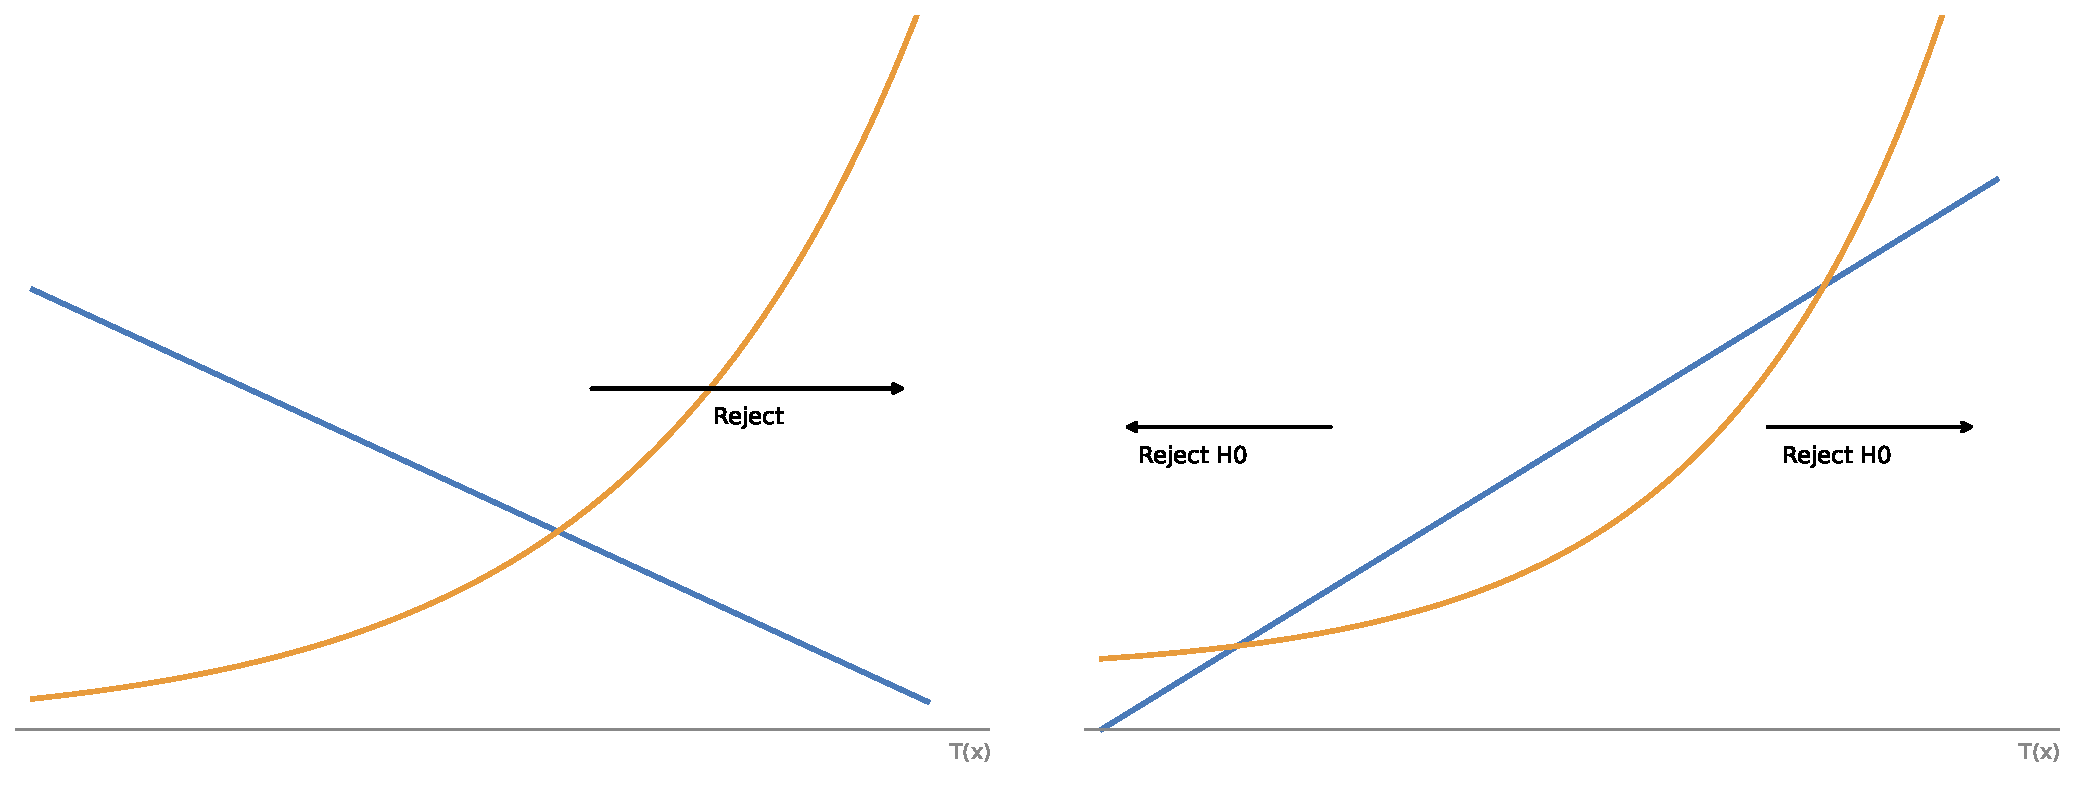
\includegraphics[width=0.9\linewidth]{figures/rejection_regions.pdf}
    \caption{Rejection Regions}
    \label{fig:rejection_regions}
\end{figure}


The first possibility will not give rise to an unbiased test, because the result would be a one-sided test with monotone power functions. Therefore any optimal $\phi$ is of the form
\[
\phi(x) = \begin{cases} 1 & \text{if } T(x) > C_1 \text{ or } T(x) < C_2 \\ \gamma_i & \text{if } T(x) = C_i \\ 0 & \text{otherwise} \end{cases}.
\]
A simplification is possible if $T(x)$ is symmetrically distributed under $\theta_0$. Then the optimal test rejects whenever $|T(x)| > \text{const}$. Such tests are called \textbf{equitailed tests}.

\subsubsection{UMP Invariant Tests}
\begin{exam}
Suppose that we observe $X = (X_1, \ldots, X_d)$, with independent coordinates $X_i \sim \mathcal{N}(\theta_i, 1)$ and that we are interested in the hypothesis testing problem
\[
H_0 : \theta_1 = \ldots = \theta_d = 0 \quad \text{vs.} \quad H_1 : \exists i \in \{1, \ldots, d\} : \theta_i \neq 0.
\]
If we transform our data so that $X' = OX$ for $O \in \mathbb{O}(d)$, the set of $d \times d$ orthogonal matrices, i.e., the set of square matrices such that $O^\top O = OO^\top = I$, then we have $X_i' \stackrel{\text{ind}}{\sim} \mathcal{N}(\theta_i', 1)$ for $\theta' = O\theta$, and our hypothesis testing problem can be seen to be equivalent to testing
\[
H_0 : \theta_1' = \ldots = \theta_d' = 0 \quad \text{vs.} \quad H_1 : \exists i \in \{1, \ldots, d\} : \theta_i' \neq 0.
\]
Hence, when searching for a test, the \textbf{principle of invariance} would suggest constraining $\phi(X) = \phi(OX) \; \forall O \in \mathbb{O}(d)$. In this case, it can be checked that $\phi$ is invariant in this way iff it is a function of the magnitude of the vector of samples, i.e.\ of $T = \sum_i X_i^2$. This tells us that if we only care about invariant tests, our optimality goal is to search for UMP tests among functions of $T$.

In this example, $T$ is non-central chi-squared distributed with $d$ degrees of freedom, i.e., $T \sim \chi_d^2(\psi^2)$ with a non-centrality parameter $\psi^2 = \sum_{i=1}^{d} \theta_i^2$. Thus, we can simplify the null and alternative hypotheses of our testing problem to
\[
H_0 : \psi = 0 \quad \text{vs.} \quad H_1 : \psi > 0. \quad \text{(one-sided test)}
\]
Note that we have reduced both the relevant data and the relevant parameter space for our testing problem; these are common advantages of imposing invariance constraints. To derive our UMP invariant test, we will check that the $\chi_d^2(\psi^2)$ has monotone likelihood ratios in $T$. Note that the density of non-central chi-squared distribution has the form:
\[
f(t; \psi) = e^{-\frac{\psi^2}{2}} \sum_{k=0}^{\infty} \frac{\left(\frac{\psi^2}{2}\right)^k}{k!} \cdot \frac{t^{\frac{d}{2} - 1 + k} e^{-\frac{t}{2}}}{2^{k + \frac{d}{2}} \Gamma\left(k + \frac{d}{2}\right)}.
\]
The likelihood ratio can therefore be computed as
\[
\frac{p_{\psi^2}(t)}{p_{\psi^2 = 0}(t)} = \frac{f(t; \psi)}{\frac{t^{\frac{d}{2} - 1} e^{-t/2}}{2^{\frac{d}{2}} \Gamma\left(\frac{d}{2}\right)}} = e^{-\frac{\psi^2}{2}} \sum_k c_k \left(\frac{\psi^2}{2}\right)^k t^k.
\]
where $c_k$ are non-negative constants. We can see that each term in the sum above increases in $t$, and thus the ratio as a whole is increasing in $t$. (We only need to compare each parameter value with $0$, because our null hypothesis is simple.) Thus this family has MLR, and the UMPI test rejects when $T$ is large.
\end{exam}

\subsubsection{Confidence Regions}
\begin{defn}[Confidence region]
A set $S(X)$ satisfying $\mathbb{P}_\theta[\theta \in S(X)] \ge 1 - \alpha$, for all 
$\theta \in \Omega$ is known as a $1 - \alpha$ \textbf{confidence region}, with a 
$1 - \alpha$ \textbf{confidence level}.
\end{defn}
Given a model $\mathcal{P} = \{\mathbb{P}_\theta : \theta \in \Omega\}$, we begin 
by defining an appropriate collection of tests. For each $\theta_0 \in \Omega$, let 
$\Omega_0(\theta_0)$ be a set containing $\theta_0$, where 
$\Omega_0(\theta_0) \subset \Omega$. Next, define $\phi_{\theta_0}$ to be a level 
$\alpha$ test for $H_0: \theta \in \Omega_0(\theta_0)$ vs.\ 
$H_1: \theta \notin \Omega_0(\theta_0)$, and define $A(\theta_0)$ as the acceptance 
region of $\phi_{\theta_0}$. Because $\phi_{\theta_0}$ is a level 
$\alpha$ test, and $\theta_0 \in \Omega_0(\theta_0)$, we have 
$P_\theta(X \in A(\theta)) \ge 1 - \alpha$ for all $\theta \in \Omega$.

Now consider the region $S(X) = \{\theta \in \Omega : X \in A(\theta)\}$. Since 
$P_\theta(\theta \in S(X)) = P_\theta(X \in A(\theta)) \ge 1 - \alpha$, $S(X)$ is a 
$1 - \alpha$ confidence region! Different choices of null sets $\Omega_0(\theta_0)$ 
will lead to different forms of confidence regions. For example,
\begin{enumerate}
  \item \textbf{One-sided tests} $\Omega_0(\theta_0) = \{\theta : \theta \le \theta_0\}$ 
  often yield \textbf{confidence bounds}
  \[
    S(X) = \{\theta : u(X) \le \theta\}
  \]
  where $u(X)$ denotes a data-dependent lower bound.
  \item \textbf{Two-sided tests} $\Omega_0(\theta_0) = \{\theta_0\}$ often yield 
  \textbf{confidence intervals}
  \[
    S(X) = \{\theta : u(X) \le \theta \le v(X)\},
  \]
  where $v(X)$ denotes a data-dependent upper bound.
\end{enumerate}

Intuitively, we desire a $1 - \alpha$ confidence region that is as narrow as 
possible, which we can achieve by minimizing the number of extraneous it contains. 
We make this notion precise in the following optimality property for confidence 
regions.

\begin{defn}[UMA]
A $1 - \alpha$ confidence region $S(X)$ is \textbf{uniformly most accurate} if, 
among all $1 - \alpha$ regions, $\mathbb{P}_\theta(\theta' \in S(X)) 
= \mathbb{P}_\theta(X \in A(\theta'))$ is minimized for all $(\theta, \theta')$ 
satisfying $\theta \notin \Omega_0(\theta')$.
\end{defn}

\subsection{Multiple Testing and Error Rate Control}

\subsubsection{Bonferroni’s Test and Fisher's Test}
We focus on global testing first with a number of null hypotheses $H_{0,i}$. We may care about the global null hypothesis
\[
H_0 = \bigcap_{i=1}^n H_{0,i}.
\]
We’ll assume that our p-values have the super-uniform property that (here $p_i$ is a random variable coming out of the test)
\[
\PP (p_i\le t) = t
\]
under the null hypothesis.

\begin{defn}[Bonferroni's Global Test]
Let $\alpha$ be some desired significance level (for example $0.05$), and suppose we have $n$ different hypotheses. \textbf{Bonferroni's global test} rejects the global null if
\[
\min_i p_i \leq \frac{\alpha}{n}.
\]
\end{defn}

\begin{prop}[Size of Bonferroni's Global Test]
If the $p$-values are super-uniform then Bonferroni's procedure has \textbf{size} (that is, chance of Type I error) at most $\alpha$.
\end{prop}

\begin{proof}
The probability of rejecting the null under the null hypothesis is, by a union bound and the super-uniform property
\begin{align*}
\mathbb{P}(\text{reject}) &= \mathbb{P}\left(\bigcup_{i=1}^{n} \left\{p_i \leq \frac{\alpha}{n}\right\}\right) \\
&\leq \sum_{i=1}^{n} \mathbb{P}\left(p_i \leq \frac{\alpha}{n}\right) \\
&\leq n \cdot \frac{\alpha}{n} \\
&= \alpha.
\end{align*}
\end{proof}
\begin{rem}
    Notice that this does not require any independence assumptions, and in fact if we assume p-values are uniform and independent then 
    \begin{align*}
    \mathbb{P}(\text{reject}) &=1- \mathbb{P}\left(\bigcap_{i=1}^{n} \left\{p_i \geq \frac{\alpha}{n}\right\}\right) \\
    &= 1-\left(1 - \frac{\alpha}{n}\right)^n \\
    &\approx 1- e^{-\alpha} \\
    &\approx \alpha - \frac{\alpha^2}{2} +\cdots.
    \end{align*}
\end{rem}
\begin{rem}
    But if we’re not under the global null, we will not “hug the uniform line $y=x$” anymore – sometimes (1) these sorted p-values will have a few that are extremely small and then the rest generally following the line (meaning maybe five hypotheses have very strong signals), and sometimes (2) all of the p-values will be overall deflated (too small). Bonferroni’s method is really most useful in case (1), because it will successfully reject due to the very small p-values; it will not reject the null in case (2) and thus is not a very powerful test.
\end{rem}
\begin{defn}[Fisher's Combination Test]
\textbf{Fisher's combination test} rejects the global null using a more combined measure. Specifically, we consider the test statistic
\[
T = -\sum_{i=1}^{n} 2 \log p_i,
\]
and we reject the null if $T$ is large.
\end{defn}
\begin{prop}
Assume that $p_1, \cdots, p_n$ are \textbf{independent} and uniform (for example in meta-analysis, suppose we do not have overlapping patients among the studies). Then under the null hypothesis, we have $T \sim \chi^2_{2n}$ (that is, the chi-square distribution with $2n$ degrees of freedom).
\end{prop}
Now we need to discuss which test is better. Consider a particular ``needle in a haystack" problem. 
Let $Y_i \sim N(\mu_i, 1)$ independently for $i = 1, \ldots, n$, and consider the global null
\[
H_0 : \mu_1 = \cdots = \mu_n = 0 \quad \text{vs.} \quad H_1 : \exists\, i,\ \mu_i \neq 0.
\]
Under $H_0$, Bonferroni's statistic $\max_i Y_i$ concentrates around $\sqrt{2 \log n}$. So we have power only when some $\mu_i > \sqrt{2 \log n}$ — the ``needle in a haystack'' threshold. Plotting power against $\mu_i / \sqrt{2 \log n}$, there is a sharp phase transition at $1$: power is $\approx \alpha$ below and $\approx 1$ above.

Assume the size of ``needle" $h = \sqrt{2r\log n}$. We will prove no $\alpha$-level test with some nontrivial power for $r=1-\epsilon$. The point is to avoid having a composite alternative: instead, consider the Bayesian decision problem with null hypothesis
\[
H_0 : \mu_i = 0 \text{ for all } i
\]
and a ``simple'' alternative hypothesis
\[
H_1 : \{\mu_i\} \sim \pi,
\]
where $\pi$ selects a coordinate uniformly at random and sets its mean to $\mu^{(n)}$, keeping all other means to zero.

The most powerful test in such a setting where $H_0, H_1$ are both simple hypotheses is the likelihood ratio test, and if we can show it has no power then everything else will have no power. Indeed, we have likelihoods
\[
f_0(y) = \prod_{j=1}^{n} \frac{1}{\sqrt{2\pi}} \exp\left(-\frac{1}{2} y_j^2\right), \quad f_1(y) = \frac{1}{n} \sum_{i=1}^{n} \frac{1}{\sqrt{2\pi}} \exp\left(-\frac{1}{2}(y_i - \mu)^2\right) \prod_{j : j \neq i} \frac{1}{\sqrt{2\pi}} \exp\left(-\frac{1}{2} y_j^2\right).
\]
and we want to reject when $\frac{f_1}{f_0}$ is large. What's nice is that all the terms cancel out except the shifted mean:
\[
L = \frac{1}{n} \sum_{i=1}^{n} \exp\left(Y_i \mu - \frac{1}{2} \mu^2\right).
\]
Notice that this is different from Bonferroni — it's a softmax instead of looking at the maximum, since if $\mu = \infty$ this would be completely dominated by the maximum $Y_i$. This is nice because it's just a sum of iid terms of mean $1$, and in fact if $\mu$ is small enough this likelihood concentrates:

\begin{prop}
Under the null hypothesis, if $\mu^{(n)} = (1 - \epsilon)\sqrt{2 \log n}$, then $L \to 1$ in probability as $n \to \infty$.
\end{prop}
Under such proposition, if we set threshold $T_n(\alpha)$ so that $\PP_{\HH_0}(L\ge T_n(\alpha)) = \alpha$, then
\begin{align*}
\mathbb{P}(\text{type II error}) = \mathbb{P}_{H_1}(L \leq T_n(\alpha)) &= \int \mathbf{1}\{L \leq T_n(\alpha)\} \, dP_{H_1} \\
&= \int L \cdot \mathbf{1}\{L \leq T_n(\alpha)\} \, dP_{H_0} \\
&= \int \mathbf{1}\{L \leq T_n(\alpha)\} \, dP_{H_0} + \int (L - 1) \mathbf{1}\{L \leq T_n(\alpha)\} \, dP_{H_0} \\
&\to (1-\alpha) + 0,
\end{align*}
\[
\implies \mathbb{P}(\text{type I error})+\mathbb{P}(\text{type II error}) \to 1.
\]
\begin{rem}
    Consider Fisher's combination test with
    \[
    T = \sum_{i=1}^n Y_i^2 = \|\bY\|_2^2.
    \]
    By CLT, we have
    \[
    \frac{T- (n+\|\mu\|_2^2)}{\sqrt{2n+4\|\mu\|_2^2}} \sim \mc N(0,1).
    \]
    And the test is powerful when $\|\mu\| > \sqrt{2n}$ and us quite large compared to something like Bonferroni. In slightly different terminology, the main parameter that mattered here was proportional to the signal-to-noise ratio
    \[
    \text{SNR} = \frac{\text{signal power}}{\text{expected noise power}} = \frac{\|\mu\|^2}{\sigma^2 n}
    \]
\end{rem}
Our original model was that we had independent statistics $X_i$ which are $N(0, 1)$ under the null hypothesis and $N(\mu_i, 1)$ under the alternative, but now we want to extend to a setting where we have a small fraction of non-null hypotheses. Thus we will now use a simple model where
\[
H_0 : X_i \stackrel{\text{iid}}{\sim} N(0, 1), \quad H_1 : X_i \stackrel{\text{iid}}{\sim} (1 - \varepsilon) N(0, 1) + \varepsilon N(\mu, 1).
\]
In the literature we historically parameterize
\[
\varepsilon_n = n^{-\beta}, \quad \frac{1}{2} < \beta < 1,
\]
\[
\mu_n = \sqrt{2r \log n}, \quad 0 < r < 1.
\]
It turns out that we have a threshold curve
\[
\rho^*(\beta) = \begin{cases} \beta - \frac{1}{2} & \frac{1}{2} < \beta \leq \frac{3}{4}, \\ (1 - \sqrt{1 - \beta})^2 & \frac{3}{4} \leq \beta \leq 1, \end{cases}
\]
such that Neyman-Pearson has full power for $r > \rho^*(\beta)$ (that is, we can adjust the test so that the sum of type I and type II error probabilities approaches $0$) and no power for $r < \rho^*(\beta)$ (that is, for any test, the limiting sum of type I and type II error is at least $1$). A crude calculation, we get power if
\[
\max_{\text{non-null}} X_i \approx \sqrt{2r \log n} + \sqrt{2 \log n^{1-\beta}} > \sqrt{2 \log n}.
\]

\subsubsection{Higher Criticism}
In general, the whole point is that in global testing we do not know $\epsilon$ and $\mu$ and thus cannot use the NP test in the first place. We introduce Tukey’s higher criticism.
\[
HC_n^* = \max_{0 < \alpha \leq \alpha_0} \frac{F_n(\alpha) - \alpha}{\sqrt{\alpha(1 - \alpha)/n}}.
\]
\begin{rem}
    The process $\sqrt{n}(F_n(t) - t)$ will converge in distribution to a Brownian bridge, and the maximum of this rescaled Brownian bridge on $(1/n, \alpha_0)$ converges in probability to $\sqrt{2 \log \log n}$ (this is the law of the iterated logarithm). 
    And a result of Donoho and Jin says that rejecting when $HC_n^* \geq \sqrt{(1 + \varepsilon) 2 \log \log n}$ gives us $\mathbb{P}_0(\text{type I}) + \mathbb{P}_1(\text{type II}) \to 0$ for any $r$ above the detection threshold.
\end{rem}

\begin{rem}
    The main problem is that near $t = 0$, we are no longer approximately normal --- $B(n, p)$ is nicely approximated by a Gaussian if $np$ is not too small, but if $np$ is small we get something that's Poisson, which has much heavier tails. The Burk-Jones statistic is an attempt to resolve this problem, but it is not fully effective.
    The idea is that for each $t$, we can test whether $n\hat{F}_n(t) < t$ using a likelihood ratio test
    \[
    \log LR_n(t) = \begin{cases} nD(\hat{F}_n(t), t) & 0 \leq t \leq F_n(t), \\ 0 & \text{otherwise}, \end{cases}
    \]
    where $D(p_0, p_1) = p_0 \log \frac{p_0}{p_1} + q_0 \log \frac{q_0}{q_1}$, $q_i = 1 - p_i$ is the Kullback-Leibler divergence. We then define
    \[
    BJ^+ = \max_{1 \leq i \leq n/2} nD\left(p_{(i)}, \frac{i}{n}\right)
    \]
    that is, at what significance level we detect a divergence between what we see and what we expect.
\end{rem}

\subsubsection{False Discovery Rate}
We now turn to identifying which hypotheses are non-null and to controlling the false discovery rate.
\begin{table}[h]
\centering
\begin{tabular}{c|cc|c}
 & accepted & rejected & total \\
\hline
true  & $U$ & $V$ & $n_0$ \\
false & $T$ & $S$ & $n - n_0$ \\
\hline
total & $n - R$ & $R$ & $n$ \\
\end{tabular}
\end{table}

\begin{defn}[Familywise Error Rate]
The \textbf{familywise error rate (FWER)} is defined to be $\mathbb{P}(V \geq 1)$.
\end{defn}

\begin{thm}[Bonferroni's Method]
Bonferroni's method controls FWER at level $\alpha$; more specifically, if there are $n_0 \leq n$ null hypotheses, we get
\[
\mathrm{FWER} \leq \mathbb{E}[V] = \frac{n_0}{n}\alpha.
\]
\end{thm}

\begin{proof}
Since $V$ is nonnegative-integer-valued, we have $\mathbb{P}(V \geq 1) \leq \mathbb{E}[V]$. And letting $\mathcal{N}_0$ denote the set of null hypotheses, we have
\[
\mathbb{E}[V] = \mathbb{E}\left[\sum_{i \in \mathcal{N}_0} \mathbf{1}\left\{p_i \leq \frac{\alpha}{n}\right\}\right] = \sum_{i \in \mathcal{N}_0} \mathbb{P}\left(p_i \leq \frac{\alpha}{n}\right) = n_0 \cdot \frac{\alpha}{n},
\]
which completes the proof.
\end{proof}

Suppose we have $n$ hypotheses $H_{(1)}, \ldots, H_{(n)}$ corresponding to the \textbf{ordered} $p$-values $p_{(1)} \leq \cdots \leq p_{(n)}$ (so we choose $H_{(1)}$ to be the hypotheses with the most surprising $p$-value, and so on). Now we will compare $p$-values with an adaptive threshold based on what we've seen so far.

What we do here is called a \textbf{Holm's procedure procedure}:
\begin{itemize}
    \item First, compare with Bonferroni's threshold: if $p_{(1)} \leq \frac{\alpha}{n}$, then reject $H_{(1)}$ and move to the next step. Otherwise, reject nothing (accept all null hypotheses).
    \item Now in general for step $i$, if $p_{(i)} \leq \frac{\alpha}{n - i + 1}$, then reject $H_{(i)}$ and go to the next step ($i + 1$). Otherwise, accept \underline{$H_{(i)}, H_{(i+1)}, \ldots, H_{(n)}$} and stop.
    \item Finally, if $p_{(n)} \leq \alpha$, then we reject $H_{(n)}$; otherwise we accept it.
\end{itemize}
Notice that
\[
\{V \geq 1\} = \{\text{procedure reached } i_0\} \cap \left\{p_{(i_0)} \leq \frac{\alpha}{n - i_0 + 1}\right\},
\]
and $\mathbb{P}(V \geq 1) \leq \alpha$.

However, FWER is so stringent that we often return nothing if we require FWER control.
\begin{defn}[False Discovery Proportion \& False Discovery Rate]
The \textbf{false discovery proportion (FDP)} is given by
\[
\mathrm{FDP} = \frac{V}{\max(R, 1)} = 
\begin{cases}
V/R & R \geq 1 \\
0 & \text{otherwise}
\end{cases}
\]
(this last case is just by convention so that we can control this quantity). In general this random variable is unobserved, and the \textbf{false discovery rate (FDR)} is the expectation $\mathrm{FDR} = \mathbb{E}[\mathrm{FDP}]$ of this quantity.
\end{defn}

We'll now consider a procedure generally more powerful than Holm's procedure -- instead of Hochberg's procedure, we consider a step-up procedure with critical values $\alpha_i = \frac{\alpha i}{n}$, which is far less conservative than $\frac{\alpha}{n - i + 1}$.

\begin{thm}[Controlling FDR]
Suppose our test statistics are independent (so $p$-values are independent). Then the Benjamini-Hochberg controls the FDR at level $\alpha$. More precisely, we actually have the expression
\[
\mathrm{FDR} = \frac{n_0}{n}\alpha \leq \alpha.
\]
\end{thm}

\begin{proof}
Let $V_i = \{H_i \text{ rejected}\}$ be the indicator function for hypothesis $i$ being rejected. By definition, we have
\[
\mathrm{FDP} = \sum_{i \in \mathcal{H}_0} \frac{V_i}{R \vee 1}.
\]
Now, it suffices to show that for any null $i$, we have $\mathbb{E}\left[\frac{V_i}{R \vee 1}\right] = \frac{\alpha}{n}$. (This is somehow ``the only answer we can get'' because the nulls are uniform and thus the random variables are exchangeable.) To prove this claim, notice that we can do casework over the value of $R$ and write
\[
\frac{V_i}{R \vee 1} = \sum_{k=1}^{n} \frac{V_i \mathbf{1}\{R = k\}}{k} = \sum_{k=1}^{n} \frac{\mathbf{1}\left\{p_i \leq \frac{\alpha k}{n}\right\} \mathbf{1}\{R = k\}}{k},
\]
since assuming $R = k$, we know the threshold for rejection is $\frac{\alpha k}{n}$. Notice that on the event $p_i \leq \frac{\alpha k}{n}$, changing $p_i$ to zero doesn't change the threshold, meaning whenever we reject $H_i$, the number (and identity) of rejections is the same. So we can write the above expression as
\[
\sum_{k=1}^{n} \frac{\mathbf{1}\left\{p_i \leq \frac{\alpha k}{n}\right\} \mathbf{1}\{R(p_i \to 0) = k\}}{k},
\]
where this notation means that we set this null $p$-value to zero. Now we can take the expectation of this quantity conditioned on all other $p$-values -- the only randomness is in $p_i$ here, so
\begin{align*}
\mathbb{E}\left[\frac{V_i}{R \vee 1} \,\bigg|\, p_1, \ldots, p_{i-1}, p_{i+1}, \ldots, p_n\right] 
&= \sum_{k=1}^{n} \frac{\frac{\alpha k}{n} \mathbf{1}\{R(p_i \to 0) = k\}}{k} \\
&= \sum_{k=1}^{n} \frac{\alpha}{n} \mathbf{1}\{R(p_i \to 0) = k\} \\
&= \frac{\alpha}{n}.
\end{align*}
Then finally taking the expectation over the last $p$-value yields the result.
\end{proof}

Consider dependency,
\begin{thm}[Guo-Rao '08]
Let $S(n) = 1 + \frac{1}{2} + \cdots + \frac{1}{n} \approx \log n + 0.577$ be the $n$th harmonic number. Then there are joint distributions where the FDR of the Benjamini-Hochberg procedure $BH(\alpha)$ is at least $\min(1, \alpha S(n))$.
\end{thm}

\begin{thm}[Benjamini-Yekutieli '01]
Under dependence of $p$-values, the $BH(\alpha)$ procedure does control at level $\alpha S(n)$; in fact,
\[
\mathrm{FDR} \leq \alpha S(n) \cdot \frac{n_0}{n}.
\]
\end{thm}

The following proof is also by Professor Cand\'es and a former student:

\begin{proof}
Let $\alpha_i = \frac{i\alpha}{n}$; much like in the proof before, it suffices to show that $\mathbb{E}\left[\frac{V_i}{R \vee 1}\right] = \frac{\alpha}{n} S(n)$. We again have
\[
\frac{V_i}{R \vee 1} = \sum_{k=1}^{n} \frac{\mathbf{1}\{p_i \leq \alpha_k\} \mathbf{1}\{R = k\}}{k},
\]
and we look at where $p_i$ can fall. Summing over the possible ranks it can take on, we have
\[
\sum_{k=1}^{n} \sum_{\ell=1}^{k} \frac{\mathbf{1}\{\alpha_{\ell-1} \leq p_i \leq \alpha_\ell\} \mathbf{1}\{R = k\}}{k} = \sum_{\ell=1}^{k} \sum_{k \geq \ell} \frac{\mathbf{1}\{\alpha_{\ell-1} \leq p_i \leq \alpha_\ell\} \mathbf{1}\{R = k\}}{k}
\]
just by swapping the order of summation. But now if we do the $k$-sum first, we're just looking at the probability of getting a particularly high number of rejections, so this simplifies to
\[
\sum_{\ell=1}^{n} \frac{\mathbf{1}\{R \geq \ell\}}{R} \mathbf{1}\{p_i \in [\alpha_{\ell-1}, \alpha_\ell]\}.
\]
Everything so far has been an equality, so ``nothing interesting'' has happened yet. But now we can simplify the first fraction to be bounded by $\frac{1}{\ell}$,
\[
\sum_{\ell=1}^{n} \frac{1}{\ell} \mathbf{1}\{p_i \in [\alpha_{\ell-1}, \alpha_\ell]\} = \sum_{\ell=1}^{n} \frac{1}{\ell} \frac{\alpha}{n} = S(n) \frac{\alpha}{n},
\]
and then the rest of the proof proceeds as before. What's surprising is that the result of Guo and Rao shows that there are distributions of $p$-values for which this inequality is indeed tight!
\end{proof}

\subsubsection{E-Values}
\begin{exam}
Consider the following situation (which is real): research group $A$ tests a medication and gets a promising but not conclusive result (whatever that means -- perhaps it's risky to go to trial). Then research group $B$ tests again on new data, but it's still not clear, so research group $C$ tests next (again on new data). We then want to understand how to combine these test results together even when we aren't following a fixed plan.
\end{exam}
Another bad news is in many cases we can not get p-values easily.
The e-value is a generic replacement of the p-value which will handle this problem of optional continuation.

\begin{defn}
Recall that a null hypothesis $\mathcal{H}_0$ is basically a collection of probability measures. An \emph{$e$-variable $E$ for testing $\mathcal{H}_0$} is a nonnegative random variable such that
$$\sup_{P_0 \in \mathcal{H}_0} \mathbb{E}_{P_0}[E] \leq 1.$$
A realization of an $e$-variable is called an \emph{$e$-value}. Meanwhile, a \emph{$p$-variable for testing $\mathcal{H}_0$} is a nonnegative random variable that satisfies
$$\sup_{P_0 \in \mathcal{H}_0} \mathbb{P}_{P_0}(P \leq \alpha) \leq \alpha$$
for all $\alpha \in (0,1)$, and a realized value of a $p$-variable is a $p$-value.
\end{defn}

\begin{prop}
For any $e$-value $E$, the random variable $E^{-1}$ is a conservative $p$-value (meaning that it is a $p$-value with wiggle room).
\end{prop}
\begin{proof}
Indeed, we have
$$\mathbb{P}\left(\frac{1}{E} \leq \alpha\right) = \mathbb{P}\left(E \geq \frac{1}{\alpha}\right) \leq \frac{\mathbb{E}[E]}{1/\alpha} \leq \alpha.$$
\end{proof}

\begin{exam}
We'll be looking at \textbf{safety under optional continuation} in this lecture: suppose $(X_1, Z_1), (X_2, Z_2), \ldots$ is our data, where $Z_i$ is some ``side information'' (for example, whether we have enough money to keep running experiments). Suppose that the data comes in batches of size $n_1, n_2, \ldots$, and $N_t = \sum_{i=1}^{t} n_i$ is the size of the data we have so far.
\end{exam}

We'll establish an $e$-value $E_1$ on the first batch. From there, we evaluate an $e$-value $E_2$ on the next batch, but only if the outcome is in a certain range (promising but not conclusive) and the external factors take on certain values (things that we cannot plan) -- otherwise we stop early. Then depending on the outcomes and external factors up until the second batch, we decide whether or not to compute $E_3$, and so on. But the point is that after $\tau$ total data batches, \textbf{the final result we report is the product}
\[
V_\tau = \prod_{i=1}^{\tau} E_i.
\]
In particular, we're allowed to choose whether to continue on depending on whether each individual $E_i$ is above some threshold of our choice, and the point is that we'll still be able to control the type I error:

\begin{thm}
Regardless of the stop-continue rule, as long as $\tau$ is a stopping time, $V_\tau$ is itself an $e$-value. More formally, let $\mathcal{F}_t$ be a filtration. Suppose that for all $t$, the conditional $e$-variable $E_t$ is a nonnegative random variable which is $\mathcal{F}_t$-measurable, and such that for all $P_0 \in \mathcal{H}_0$ we have $\mathbb{E}_{P_0}[E_t | \mathcal{F}_{t-1}] = 1$. (This is easy to check in practice.) Then $V_t = \prod_{i \leq t} E_i$ is a nonnegative supermartingale under the null. Thus by the optional stopping theorem, for any stopping time $\tau$ with respect to the filtration, $V_\tau = \prod_{t=1}^{\tau} E_t$ is an $e$-value. (In particular, $V_t$ is an $e$-value for each fixed $t$.)
\end{thm}

Now we focus on multiple testing.
\begin{defn}
In the \textbf{e-BH procedure}, we reject the hypotheses of the largest $\hat{k}$ e-values, where
\[
\hat{k} = \max\left\{i : \frac{i e_{(i)}}{n} \geq \frac{1}{\alpha}\right\}.
\]
\end{defn}

\begin{rem}
We should be careful that $\frac{1}{p}$ is not an $e$-value in general (in fact its expectation need not be finite), even though $\frac{1}{e}$ is always a $p$-value.
\end{rem}

\begin{thm}[Wang--Ramdas '20]
The $e$-BH procedure has FDR at most $\frac{n_0 \alpha}{n}$, and no independence assumption is required.
\end{thm}

\subsection{Causal Inference}
\subsubsection{Randomized Controlled Trials}
A traditional view holds that statistics is concerned with inferring correlations or associations among variables. From this perspective, causal inference appears to have no place in statistics. In this section, however, we will discuss several statistical methods for estimating causal effects in both randomized experiments and observational studies.

We define the causal effect of a treatment via potential outcomes. For a binary treatment $w \in \{0, 1\}$, we define potential outcomes $Y_i(1)$ and $Y_i(0)$ corresponding to the outcome the $i$-th subject would have experienced had they respectively received the treatment or not. The \textbf{causal effect of the treatment on the $i$-th unit} is then
\[
    \Delta_i = Y_i(1) - Y_i(0).
\]
The fundamental problem in causal inference is that only one treatment can be assigned to a given individual, and so only one of $Y_i(0)$ and $Y_i(1)$ can ever be observed. Thus, $\Delta_i$ can never be observed.
Now, although $\Delta_i$ itself is fundamentally unknowable, we can (perhaps remarkably) use \textbf{randomized experiments} to learn certain properties of the $\Delta_i$. In particular, large randomized experiments let us recover the average treatment effect (ATE)
\[
    \tau = \mathbb{E}\left[Y_i(1) - Y_i(0)\right].
\]

\textit{}When an RCT is unavailable, we can use observational data  $(X_i,Y_i,W_i)$ to construct an estimator for the ATE. 
Considering the \textbf{propensity score}
\[
e(x) = \mathbb{P}\left[W_i = 1 \mid X_i = x\right],
\]
and we construct the inverse-propensity weighting estimator
\[
\hat{\tau}_{IPW} = \frac{1}{n} \sum_{i=1}^{n} \left( \frac{W_i Y_i}{\hat{e}(X_i)} - \frac{(1 - W_i) Y_i}{1 - \hat{e}(X_i)} \right).
\]
\begin{rem}
    IPW relies on the unconfoundedness assumption
    \[
    \{Y_i(0), Y_i(1)\} \indep W_i \mid e(X_i).
    \]
    Many real-world policies assign treatment by a sharp rule on a running variable (e.g., scholarships above a GPA cutoff). Units just above and below the cutoff are nearly identical in all other respects, so the discontinuity creates a local "as-if randomized" experiment.
\end{rem}



\subsection{Conformal prediction}
\subsubsection{Fundamentals}
Suppose $X_1, \ldots, X_n$ are iid samples from some probability distribution $P$, and $Y_1, \ldots, Y_m$ are iid samples from some other probability distribution $Q$. Our goal is to test the hypothesis that $P = Q$ even if we don't know either of the distributions.
The strategy we learn in early statistics is that we should choose a test statistic $T$ (for example we can let $T = |\overline{X} - \overline{Y}|$) and reject the null based on whether $T$ is unusually large. The question we need to ask is ``how large does $T$ need to be,'' and typically this is where permutation tests are introduced: we compare $T$ to how the statistic would look \textbf{if we were to permute the data}.

Formally, we introduce the following (randomized) \textbf{permutation distribution}: choose $M$ uniform permutations $\sigma_1, \ldots, \sigma_M$ from $S_{n+m}$ (the set of permutations acting on a list of $n + m$ objects), and we will have these permutations act on the vector
\[
Z = (X_1, \ldots, X_n, Y_1, \ldots, Y_m).
\]
Specifically, the $\sigma_i$s will shuffle the entries of $Z$, and then we evaluate the test statistic on the permuted entry. So we always take the average of the first $n$ entries and the average of the last $m$ entries after permuting, and we find their absolute difference; in other words, we compare
\[
T(Z) = \left|\overline{Z_{1:n}} - \overline{Z_{n+1:n+m}}\right|
\]
to the corresponding values of $T(Z_\sigma)$, and the $p$-value will essentially be the relative rank of $T(Z)$ compared to $T(Z_{\sigma_1})$ through $T(Z_{\sigma_M})$:
\[
p = \frac{1 + \sum_{i=1}^{M} \mathbf{1}\{T(Z_{\sigma_i}) \geq T(Z)\}}{1 + M}.
\]
Under the null, this is either uniformly distributed on $\left\{\frac{1}{M+1}, \frac{2}{M+1}, \ldots, \frac{M+1}{M+1}\right\}$ or biased upward due to ties (because under the null we have exchangeability of the vector $Z$). Thus it is indeed a $p$-value, and notice that this doesn't rely on us needing to know the distribution of $T$ at all.
Given a set of permutations $S$, consider the quantity
\[
p = \frac{1 + \sum_{\sigma \in S} \mathbf{1}\{T(Z_\sigma) \geq T(Z)\}}{1 + |S|}.
\]
If the variables are exchangeable, then $Z_\sigma$ has the same distribution as $Z$ and thus $T(Z_\sigma)$ has the same distribution as $T(Z)$. We are interested in what sets of permutations $S$ yield a valid $p$-value.
Here are the answers:
\begin{center}
\begin{tabular}{c|c}
$S$ & $p$-value? \\
\hline
all permutations ($S_n$) & Yes \\
iid samples from $S_n$ & Yes \\
an arbitrary fixed subset of $S_n$ & No \\
iid samples from an arbitrary fixed subset & No \\
a subgroup of $S_n$ & Yes \\
iid samples from a subgroup of $S_n$ & Yes \\
\end{tabular}
\end{center}

\begin{exam}[Conformal Prediction]
In predictive inference, we take some set of training samples $(X_1, Y_1), \ldots, (X_n, Y_n)$ which are iid from some distribution $P$. We then get a test sample $X_{n+1}$, and our goal is to construct, from the training samples, a prediction interval for $Y_{n+1}$ with prescribed coverage. That is, we want some $C$ so that
\[
\mathbb{P}(Y_{n+1} \in C(X_{n+1})) \geq 1 - \alpha.
\]
\end{exam}

Note that this is not a confidence interval -- this is an observation we have not seen yet, and it's interesting that we can solve this problem at all. In fact, the way we can do so is through permutation tests! We hypothesize a value of $Y_{n+1}$ and test for exchangeability by computing
\[
p^y = \frac{1}{(n+1)!} \sum_{\sigma \in S_{n+1}} \mathbf{1}\{T(Z^y_\sigma) \geq T(Z^y)\},
\]
where $Z^y = \{(X_1, Y_1), \ldots, (X_n, Y_n), (X_{n+1}, y)\}$. Then setting $y \in C(X_{n+1})$ if and only if $p^y \geq \alpha$, we claim this is a valid prediction interval regardless of our choice of $T$. Indeed, $Y_{n+1}$ itself will be in the confidence interval if and only if $p^{Y_{n+1}} \geq \alpha$, but we've already shown that $p^{Y_{n+1}} \stackrel{\text{sto}}{\geq} U$ and thus we are done.

The motivation for conformal prediction is that we want some uncertainty in our prediction and some way of quantifying accuracy.

\subsubsection{Approaches}
\textbf{Full conformal prediction}  is typically done as follows: we fit a model $\hat{\mu}(\cdot) = \mathcal{A}(Z^y)$ to $Z^y = ((X_1, Y_1), \ldots, (X_n, Y_n), (X_{n+1}, y))$ which satisfies the symmetry assumption (for example in random forests, it doesn't matter what order we pass in the data, and this is true of most algorithms), and we define $T(Z^y) = |y - \hat{\mu}(X_{n+1})|$ to be the residual. Replacing $T$ with what we have, we thus get a $p$-value
\[
p^y = \frac{1}{n+1} \sum_{i=1}^{n+1} \mathbf{1}\{|Y_i - \hat{\mu}(X_i)| \geq |y - \hat{\mu}(X_{n+1})|\} = \frac{1}{n+1} \sum_{i=1}^{n+1} \mathbf{1}\{R^y_i \geq R^y_{n+1}\}.
\]
and again we include $y$ in the interval if and only if $p^y\ge \alpha$. This is all computationally intensive – every time we fit the model we might need to do a lot of computation, and in fact the prediction interval can be a disjoint set of intervals instead.

We introduce \textbf{split conformal prediction} then. This is a special case where we have $n$ data points and we do sample splitting: we learn a model $\hat{\mu}$ with the first split (also called a ``fold''), and on the second split we calculate out-of-sample residuals (that is, learn the distribution of the residuals $R_i = |Y_i - \hat{\mu}(X_i)|$). Then the test residual relates to this second split by keeping track of quantiles, and the point is that we separately do training and calibration and form our interval from points that have all not been used for training.

Formally, we compute a score function $S(x, y) = |y - \hat{\mu}(x)|$ by fitting a model on an independent training set. Once we have this, we use a distinct calibration set of size $n$ to find typical size of residuals
\[
S_i = S(X_i, Y_i), \quad S^y_{n+1} = S(X_{n+1}, y).
\]
The point is that if $y = Y_{n+1}$ these points should all be indistinguishable (they're from the same distribution), and now we include $y$ if
\[
p^y = \frac{1}{n+1} \sum_{i=1}^{n} \mathbf{1}\{S_i \geq S^y_{n+1}\} \geq \alpha.
\]
And this result now holds conditionally on the training set, since for all purposes $\hat{\mu}$ is fixed.

\begin{rem}
    Other methods to estimate $\hat{\mu}$ include Leave-One-Out and Cross-Validation.
\end{rem}


\subsection{Application: Watermark Detection}
\todo
\newpage
\section{Classical Statistical Model}
Up to this point, we have acquired many statistical tools, and it is now time to step back and look at the whole picture. First, we collect a set of data points $(x_i, y_i)$. We then select an appropriate statistical model for the data, typically a parameterized one, and find the optimal parameters. Finally, we validate the model and use it to make predictions at new data points. In this section, we will discuss several statistical models. The section is organized as follows:
\begin{enumerate}
    \item Regression
    \item Classification
    \item Trees and Weak Learners
    \item Cross-Validation
    \item Time Series
\end{enumerate}

This section mainly follows STAT254 (UC Berkeley), Statistics Learning (PKU, taught by Fang Yao) and STAT153 (UC Berkeley).
I would also like to extend my heartfelt thanks to my STAT254 professor, Ryan Giordano, who has offered me countless insights and inspiration in the field of statistics.


\subsection{Regression}

\subsubsection{Fundamentals}
In general, we can define the ``loss'' of guessing $\hat{y}$ when the true value was is $y$ as
\[
\mathscr{L}(\hat{y}, y) = \mathscr{L}(f(\bx), y)
\]
We want to find $f(\cdot)$ so that $\mathscr{L}(f(\bx), y)$ is as small as possible. But the loss for a particular $f$ may depend on $\bx_{\mathrm{new}}$, since different $\bx_{\mathrm{new}}$ are associated with different distributions of $y_{\mathrm{new}}$. It follows that it doesn't make sense to minimize the loss --- instead we want to minimize the \emph{risk},
\[
\mathscr{L}(f) := \mathbb{E}\left[\mathscr{L}(f(\bx), y)\right] \qquad \text{(Risk)}.
\]
So we would like to find
\[
f^{\star}(\cdot) := \operatorname*{argmin}_{f} \mathscr{L}(f) = \operatorname*{argmin}_{f} \mathbb{E}\left[\mathscr{L}(f(\bx), y)\right].
\]

We'll consider square loss first:
\[
l(\bx, y) = \frac 1 2(y - f(\bx))^2 \quad \hat{\mathcal{L}}(f) = \frac{1}{N} \sum_{i=1}^N l(\bx_i,y_i).
\]
We cannot actually compute $f^*$, a general question is how to calculate the gap between $f^*$ and $\hat f$.
\[
0 \leq \mathscr{L}(\hat{f}) - \mathscr{L}(f^*)
= \underbrace{\mathscr{L}(\hat{f}) - \hat{\mathscr{L}}(\hat{f})}_{\text{Difficult term!}}
+ \underbrace{\hat{\mathscr{L}}(\hat{f}) - \hat{\mathscr{L}}(f^*)}_{\text{Negative term}}
+ \underbrace{\hat{\mathscr{L}}(f^*) - \mathscr{L}(f^*)}_{\text{LLN term}}.
\]
It is called generalization error and the term $\mathcal{L}(\hat f) - \hat{\mathcal{L}}(\hat f)$ can be bounded $\sup_{f} [\mathcal{L}(f) - \hat{\mathcal{L}}(f)]$, which will be discussed in the later sections.

We begin with linear regression model:
\[
y_n = \beta_1 x_{n1} + \beta_2 x_{n2} + \ldots + \beta_P x_{nP} + \varepsilon_n = \underbrace{\bx_n^\top \bbeta}_{f(\bx_n)} + \epsilon_n, \quad \text{For } n = 1, \ldots, N.
\]
where we use $N$ to denote the number of data and $P$ to denote the number of features.
To get the optimal estimator $\hat{\bbeta}$, we let
\[
0 = \frac{\partial}{\partial \bbeta} \mathcal{L}(\bbeta) \implies \bX^\top (\bY-\bX\bbeta)=0 \implies \hat{\bbeta} = (\bX^\top \bX)^{-1} \bX^\top \bY.
\]

In the general case, the optimal function is $f^*(\bx) = \EE[y \mid \bx]$, and the linear model approximates this conditional expectation as $\EE[y \mid \bx] = \bbeta^\top \bx$. To expand the function space and improve expressiveness, we sometimes apply a feature mapping to $\bx$. A simple example of a feature mapping is the polynomial mapping.
\paragraph{Splines}
For a partition $\zeta_0, \ldots, \zeta_K$ of the $x$-axis, define the indicator regressors
\[
\mathbf{z}_n^0 = \begin{pmatrix}
\mathrm{I}(\zeta_0 \leq x < \zeta_1) \\
\vdots \\
\mathrm{I}(\zeta_{K-1} \leq x < \zeta_K)
\end{pmatrix}.
\]
Regressing $y_n \sim \mathbf{z}_n^0$ produces a \emph{piecewise constant} fit, returning the average of training responses within each interval.
Indicator regressors give discontinuous fits with zero derivative. To obtain a piecewise linear fit, augment with
\[
\mathbf{z}_n^1 = \begin{pmatrix}
\mathrm{I}(\zeta_0 \leq x < \zeta_1)(x - \zeta_0) \\
\vdots \\
\mathrm{I}(\zeta_{K-1} \leq x < \zeta_K)(x - \zeta_{K-1})
\end{pmatrix}.
\]
Regressing $y_n \sim \mathbf{z}_n^0 + \mathbf{z}_n^1$ yields a separate first-order Taylor approximation within each segment.
Generalizing to degree $p$,
\[
\mathbf{z}_n^p = \begin{pmatrix}
\mathrm{I}(\zeta_0 \leq x < \zeta_1)(x - \zeta_0)^p \\
\vdots \\
\mathrm{I}(\zeta_{K-1} \leq x < \zeta_K)(x - \zeta_{K-1})^p
\end{pmatrix},
\]
gives a $p$-th order polynomial fit within each bucket.

\paragraph{Bias and Variance Trade-off}
Let’s decompose this target $\mathbb{E}\left[(\hat{f}(\mathbf{x}_{\mathrm{new}}) - y_{\mathrm{new}})^2\right]$.
\begin{align*}
\mathbb{E}\left[(\hat{f}(\mathbf{x}_{\mathrm{new}}) - y_{\mathrm{new}})^2\right]
&= \mathbb{E}\left[(\hat{f}(\mathbf{x}_{\mathrm{new}}) - \bar{f}(\mathbf{x}_{\mathrm{new}}) + \bar{f}(\mathbf{x}_{\mathrm{new}}) - f^{\star}(\mathbf{x}_{\mathrm{new}}) + f^{\star}(\mathbf{x}_{\mathrm{new}}) - y_{\mathrm{new}})^2\right] \\
&= \underbrace{\mathbb{E}\left[(\hat{f}(\mathbf{x}_{\mathrm{new}}) - \bar{f}(\mathbf{x}_{\mathrm{new}}))^2\right]}_{\text{``variance''}} + \underbrace{\mathbb{E}\left[(\bar{f}(\mathbf{x}_{\mathrm{new}}) - f^{\star}(\mathbf{x}_{\mathrm{new}}))^2\right]}_{\text{``bias''}} + \underbrace{\mathbb{E}\left[(f^{\star}(\mathbf{x}_{\mathrm{new}}) - y_{\mathrm{new}})^2\right]}_{\text{``irreducible error''}}.
\end{align*}
Define $M_{xx} = \EE [\bx^\top \bx]$ and $M_{xy} = \EE[\bx^\top y]$. Then $\bbeta = M_{xx}^{-1}M_{xy}$. By CLT,
\[
\hat{\bbeta} - \bbeta^*
= \left(\frac{1}{N} \sum_{n=1}^{N} \mathbf{x}_n \mathbf{x}_n^\top\right)^{-1} \frac{1}{N} \sum_{n=1}^{N} \mathbf{x}_n (y_n - \mathbf{x}_n^\top \mathbf{\beta}^*), \quad
\sqrt{N}(\hat{\bbeta} - \bbeta^*) \to \mathcal{N}(0, M_{xx}^{-1} U M_{xx}^{-1}),
\]
where $U := \operatorname{Cov}(\bx_n \epsilon_n)$. We have
\[
N \cdot\text{Variance} \approx \operatorname{tr}(M_{xx}^{-1/2} U M_{xx}^{-/2}) = \sigma^2\operatorname{tr}(I_P) = P\sigma^2 \implies \text{Variance} \approx \frac{P\sigma^2}{N}.
\]

\subsubsection{Ridge ($L_2$) and Lasso ($L_1$) Regression}
When $P \gg N$, $\bX^\top\bX$ is non-invertible, and the model is prone to overfitting---a common phenomenon in this regime. A simple remedy is to introduce a penalty term. We begin with the $L_2$ penalty.
\[
\mathcal{L}_{ridge}(\bbeta, \lambda) = \|\bY-\bX^\top\bbeta\|_2^2 + \lambda \|\bbeta\|_2^2 \implies \hat\bbeta_{ridge} = (\bX^\top \bX + \lambda \bI)^{-1} \bX^\top \bY.
\]
Assume $\bY = \bX^\top \bbeta^* + \bvarepsilon$ with $\mathbb{E}[\bvarepsilon] = \bzero$ and $\mathrm{Cov}(\bvarepsilon) = \sigma^2 \bI$. Let the singular value decomposition give $\bX^\top\bX = \bV \bSigma^2 \bV^\top$ with $\bSigma^2 = \mathrm{diag}(d_1, \ldots, d_P)$, so that $(\bX^\top\bX + \lambda \bI)^{-1} = \bV (\bSigma^2 + \lambda \bI)^{-1} \bV^\top$.

A direct computation gives
\[
\mathbb{E}[\hbbeta_{\text{ridge}}] - \bbeta^* = -\lambda \bV (\bSigma^2 + \lambda \bI)^{-1} \bV^\top \bbeta^*, \qquad \mathrm{Cov}(\hbbeta_{\text{ridge}}) = \sigma^2 \bV \, \mathrm{diag}\!\left(\frac{d_j}{(d_j+\lambda)^2}\right) \bV^\top,
\]
which yields
\[
\text{Bias: }\| \mathbb{E}[\hbbeta_{\text{ridge}}] - \bbeta^* \|_2^2 = \sum_{j=1}^{P} \frac{\lambda^2}{(d_j + \lambda)^2} (\bv_j^\top \bbeta^*)^2, \qquad \text{Variance: }\mathrm{tr}\,\mathrm{Cov}(\hbbeta_{\text{ridge}}) = \sigma^2 \sum_{j=1}^{P} \frac{d_j}{(d_j + \lambda)^2}.
\]
As $\lambda$ increases, the variance decreases while the bias increases.

Another choice is $L_1$ penalty, which we called LASSO,
\[
\mathcal{L}_{lasso}(\bbeta, \lambda) = \|\bY-\bX^\top\bbeta\|_2^2 + \lambda \|\bbeta\|_1.
\]
\begin{rem}
    LASSO favors \textbf{sparse} solutions, whereas Ridge spreads weight more evenly across coefficients. This makes LASSO a natural tool for variable selection: by tuning $\lambda$, one can identify the salient predictors as those with nonzero coefficients.
\end{rem}

\subsubsection{Kernel Methods}
Consider the Ridge Regression, by some Mathematics tricks
\[
\hat\bbeta_{ridge} = (\bX^\top \bX + \lambda \bI_P)^{-1} \bX^\top \bY = \bX(\bX \bX^\top + \lambda \bI_N)^{-1}  \bY.
\]
Note that we have replaced an $P\times P$ inverse with an $N\times N$ inverse, and may reduce computation (in some case). $\bX \bX^\top = (x_i^\top x_j)_{i,j}$, replace $x_i^\top x_j$ into $k(x_i,x_j)$, and we have kernel function.

\begin{defn}[Reproducing Kernel Hilbert Space]
Let $\cX$ be an arbitrary set and $\cH$ a Hilbert space of real-valued functions on $\cX$. We say $\cH$ is a \emph{reproducing kernel Hilbert space} (RKHS) if there is a kernel $k : \cX \times \cX \mapsto \mathbb{R}$ such that
\begin{itemize}
    \item $\forall x \in \cX,\ k(\cdot, x) \in \cH$.
    \item \emph{Reproducing property:} $\forall x \in \cX,\ f \in \cH,\ \langle f, k(\cdot, x) \rangle_\cH = f(x)$.
\end{itemize}
\end{defn}

For a kernel $k : \cX \times \cX \to \mathbb{R}$, we define an integral operator $\cT_k : L^2_\mu(\cX) \to L^2_\mu(\cX)$ as follows
\[
\cT_k f(x) = \mathbb{E}_{x' \sim \mu}[k(x, x') f(x')].
\]

\begin{thm}[Mercer's theorem]
Let $k$ be a continuous kernel on a \textbf{compact set} $\cX$. There exist an orthonormal basis $\{e_j\}_{j=1}^\infty$ of $L^2_\mu(\cX)$ such that $\forall x, x' \in \cX$,
\[
k(x, x') = \sum_{j=1}^{\infty} \lambda_j e_j(x) e_j(x').
\]
The convergence is uniform on $\cX \times \cX$ and absolute for each $(x, x') \in \cX \times \cX$.
\end{thm}
\begin{rem}
    From this perspective, an RKHS can be viewed as a subspace of $L_2$. The faster the eigenvalues $\lambda_j$ decay, the smaller the RKHS---and correspondingly, the smoother the functions it contains.
\end{rem}

This theorem ensures the existence of an eigendecomposition of a kernel $k$, i.e., the corresponding integral operator $\cT_k$. Note that $(\lambda_j)_{j \geq 1}$ and $(e_j)_{j \geq 1}$ are the eigenvalues and eigenfunctions of the integral operator $\cT_k$ in the sense that
\begin{itemize}
    \item $\cT_k e_j = \lambda_j e_j$, i.e., $\mathbb{E}_{x' \sim \mu}[k(x, x') e_j(x')] = \lambda_j e_j(x)$.
    \item $\langle e_i, e_j \rangle_{L^2_\mu(\cX)} = \mathbb{E}_{x \sim \mu}[e_j(x) e_i(x)] = \delta_{i,j}$.
\end{itemize}

\paragraph{Feature map.} Mercer's theorem gives a feature map for the kernel $k$. Let
\[
\Phi : \cX \to \ell^2, \qquad \Phi(x) = \left(\sqrt{\lambda_1} e_1(x), \sqrt{\lambda_2} e_2(x), \ldots, \sqrt{\lambda_j} e_j(x), \ldots\right)^\top.
\]
Then,
\[
k(x, x') = \sum_{j=1}^{\infty} \sqrt{\lambda_j} e_j(x) \sqrt{\lambda_j} e_j(x') = \langle \Phi(x), \Phi(x') \rangle_{\ell^2}.
\]

\begin{thm}[Spectral representation of RKHS]
Let $k$ be a continuous kernel on a compact set $\cX$, and $\{e_j\}$ be the orthonormal basis given in Mercer's theorem. Define
\[
\cH = \left\{ f = \sum_j a_j e_j : \sum_j \frac{a_j^2}{\lambda_j} < \infty \right\},
\]
with the inner product
\[
\left\langle \sum_j a_j e_j, \sum_j b_j e_j \right\rangle_{\cH} = \sum_j \frac{a_j b_j}{\lambda_j}.
\]
Then, $\cH$ is the RKHS $\cH_k$.
\end{thm}

\subsection{Classification}
\subsubsection{Fundamentals}
Let us now turn to classification problems. Like regression, we assume we get IID observations $z_n = (\mathbf{x}_n, y_n)$, but now with the difference that $y$ takes one of a set of unordered distinct values, which I will call $\mathcal{Y}$. The simplest case is where $y$ takes one of two values, which I will sometimes call ``binary classification''. As before, we wish to use $\mathbf{x}$ to guess what $y$ is. As we will see shortly, there are more choices to what $f$ should even be for classification than there are for regression.

Ultimately, we need a mapping $\mathbf{x} \mapsto \mathcal{Y}$, so we might take $\hat{y}(\mathbf{x}) \in \mathcal{Y}$. Necessarily, the loss function must take in two values in $\mathcal{Y}$---the guess and the truth---and return a real number. Formally, $\mathscr{L}: \mathcal{Y} \times \mathcal{Y} \mapsto \mathbb{R}$, which can be fully represented as a $|\mathcal{Y}| \times |\mathcal{Y}|$ matrix.
The simplest case of this is called ``zero--one'' loss:
\[
\mathscr{L}_{\text{ZO}}(\hat{y}, y) = \mathrm{I}(\hat{y} \neq y) = \sum_{c \in \mathcal{Y}} \mathrm{I}(\hat{y} = c)\, \mathrm{I}(y \neq c).
\]
Note that the maximizer of the zero--one loss has a closed form:
\begin{align*}
\mathbb{E}_{\mathbb{P}(\mathbf{x},y)}\left[\mathscr{L}_{\text{ZO}}(\hat{y}, y)\right]
&= \sum_{c \in \mathcal{Y}} \mathrm{I}(\hat{y} = c)\, \mathbb{E}_{\mathbb{P}(\mathbf{x},y)}\left[\mathrm{I}(y \neq c)\right] \\
&= \sum_{c \in \mathcal{Y}} \mathrm{I}(\hat{y} = c)\bigl(1 - \mathbb{P}(y = c, \mathbf{x})\bigr) \\
&= 1 - \sum_{c \in \mathcal{Y}} \mathrm{I}(\hat{y} = c)\bigl(1 - \mathbb{P}(y = c \mid \mathbf{x})\bigr)\mathbb{P}(\mathbf{x}).
\end{align*}
Since $\mathbb{P}(\mathbf{x})$ does not depend on $c$, the best choice for $\hat{y}$ is
\begin{equation*}
\hat{y}^*(\mathbf{x}) = \operatorname*{argmax}_{c \in \mathcal{Y}} \mathbb{P}(y = c \mid \mathbf{x}).
\end{equation*}

The natural generalization of zero--one loss and functions that return categories is a function that returns a probability. For binary regression with $y \in \{0, 1\}$, we can take $\pi(\mathbf{x})$ to approximate $\mathbb{P}(y = 1 \mid \mathbf{x})$, and so take $\pi: \mathbf{x} \mapsto [0, 1]$.

\paragraph{Cross Entropy Loss}
If $\pi(\mathbf{x}) \in (0, 1)$ then we can in fact use other losses. One common choice is the negative log likelihood:
\begin{align*}
\mathscr{L}_{\text{CE}}(\pi, y)
&= -\log \mathbb{P}(y \mid \pi) \\
&= -\log \pi^{y}(1 - \pi)^{1-y} \\
&= -y \log \pi - (1-y) \log(1 - \pi) \\
&= -y \log \frac{\pi}{1 - \pi} - \log(1 - \pi).
\end{align*}
This is also known as the ``cross-entropy loss,'' since the maximum likelihood estimator is also the minimizer of the Kullback--Liebler divergence.

\paragraph{Logistic Regression}
Suppose we have $f \in \mathbb{R}$. Then
\begin{equation*}
\pi(f) = \frac{\exp(f)}{1 + \exp(f)} =: \operatorname{Expit}(f).
\end{equation*}
You can readily see that $\operatorname{Expit}(f) \in (0, 1)$.
The expit function is invertible with inverse sometimes called the ``logit'':
\begin{equation*}
\operatorname{Logit}(\pi) := \log \frac{\pi}{1 - \pi}.
\end{equation*}
Note that if you plug this formula into the cross-entropy loss,
\begin{align*}
\mathscr{L}_{\text{CE}}(\operatorname{Expit}(f), y)
&= -y \operatorname{Logit}(\operatorname{Expit}(f)) + \log(1 - \operatorname{Expit}(f)) \\
&= -y f + \log\!\left(1 - \frac{\exp(f)}{1 + \exp(f)}\right) \\
&= -y f - \log(1 + \exp(f)),
\end{align*}
And if we further take $f(\mathbf{x}) = \mathbf{\beta}^{\top} \mathbf{x}$, we get
\begin{equation*}
\mathscr{L}_{\text{CE}}(\operatorname{Expit}(\mathbf{\beta}^{\top}\mathbf{x}), y) = -y \mathbf{\beta}^{\top} \mathbf{x} - \log(1 + \exp(\mathbf{\beta}^{\top}\mathbf{x})),
\end{equation*}
which is \textbf{logistic regression}.

\paragraph{Generative modeling}
We have noted that the optimal classifier takes the form of the maximum of $\mathbb{P}(y = c \mid \mathbf{x})\mathbb{P}(\mathbf{x})$. In our reasoning above we ignored $\mathbb{P}(\mathbf{x})$ since it does not depend on $c$, and modeled $\mathbb{P}(y = c \mid \mathbf{x})$, e.g.\ using the expit function and linear models.
However, we could condition in the other direction to write
\begin{equation*}
\hat{y} = \operatorname*{argmax}_{c} \mathbb{P}(y = c \mid \mathbf{x})\mathbb{P}(\mathbf{x}) = \operatorname*{argmax}_{c} \mathbb{P}(\mathbf{x} \mid y = c)\mathbb{P}(y = c).
\end{equation*}
When we have many more data than categories, $\mathbb{P}(y = c)$ is easy to estimate:
\begin{equation*}
\mathbb{P}(y = c) \approx \frac{1}{N} \sum_{n=1}^{N} \mathrm{I}(y_n = c).
\end{equation*}
We can then attempt to model the conditional density $\mathbb{P}(\mathbf{x} \mid y = c)$ by forming density estimates the sets of points $\mathcal{X}_c := \{\mathbf{x}_n : y_n = c\}$. Density estimation is difficult in high dimensions---arguably more difficult than estimating good decision boundaries---but generative modeling can be particularly effective in low dimensions, or when something special is known about the structure of $\mathbb{P}(\mathbf{x} \mid y = c)$.

Note that the estimation $\mathbb{P}(\mathbf{x} \mid y = c)$ does not admit a ready formulation as a direct minimization of classification error. Estimation of densities is typically considered an \textbf{``unsupervised learning''} problem for this reason, even though here we would use the unsupervised learning estimate in service of a supervised learning problem.

\subsubsection{Support Vector Machines}
Suppose we have binary classification data $(\mathbf{x}_1, y_1), \ldots, (\mathbf{x}_N, y_N)$, where $y_n \in \{-1, 1\}$, and we want to find a linear decision boundary:
\begin{equation*}
\hat{y}_n = \operatorname{sign}(\mathbf{x}_n^{T} \hat{\mathbf{\beta}}).
\end{equation*}
Such a vector $\hat{\mathbf{\beta}}$ would be normal to a hyperplane that separates our predictions.
Support Vector Machines add three layers on top of this:
\begin{itemize}
    \item \textbf{Regularization}: find the separating hyperplane with maximum margin.
    \item \textbf{Soft margin}: allow for margin mistakes (e.g.\ not linearly separable).
    \item \textbf{Kernel}: expressive (possibly infinite) feature mapping.
\end{itemize}

For finite data that are linearly separable, there always are infinitely many separating hyperplanes. Which one does perceptron converge to? If it does, con implicit, so let's make it implicit and ask for a particular one. As a form of regularization, we'll ask for the one with maximum margin:
\begin{equation*}
\hat{\mathbf{\beta}}_{\text{hard}} = \operatorname*{argmax}_{\|\mathbf{\beta}\|_2 = 1,\, \gamma} \gamma \quad \text{subject to} \quad y_n \mathbf{x}_n^{T} \mathbf{\beta} \geq \gamma \quad \forall n = 1, \ldots, N.
\end{equation*}
\begin{prop}
\begin{equation*}
\hat{\mathbf{\beta}}_{\text{hard}} = \operatorname*{argmin}_{\mathbf{\beta}} \|\mathbf{\beta}\|_2 \quad \text{subject to} \quad y_n \mathbf{x}_n^{T} \mathbf{\beta} \geq 1 \quad \forall n = 1, \ldots, N.
\end{equation*}
\end{prop}

\paragraph{Soft Margin SVM}
The hard margin SVM is restricted to linearly separable data. We now introduce a soft margin (linear) SVM, which trades separability with $\|\mathbf{\beta}\|_2$:
\begin{equation*}
\hat{\mathbf{\beta}}_{\text{soft}}(\lambda) = \operatorname*{argmin}_{\mathbf{\beta}} \sum_{n=1}^{N} \max(1 - y_n \mathbf{x}_n^{T} \mathbf{\beta},\, 0) + \lambda \|\mathbf{\beta}\|_2^2.
\end{equation*}
This way, we may allow classification (or margin) mistakes for the purpose of reducing $\|\mathbf{\beta}\|_2^2$. This brings us to the familiar form of minimizing loss plus penalty.

\paragraph{Connection to hard margin SVM}
To see how soft margin SVM relates to hard margin, add slack variable $\xi_n \geq \max(1 - y_n \mathbf{x}_n^{T} \mathbf{\beta},\, 0)$ and observe that
\begin{equation*}
\hat{\mathbf{\beta}}_{\text{soft}}(\lambda) = \operatorname*{argmin}_{\mathbf{\beta}} \|\mathbf{\beta}\|_2^2 + \frac{1}{\lambda} \sum_{n=1}^{N} \xi_n \quad \text{subject to} \quad y_n \mathbf{x}_n^{T} \mathbf{\beta} \geq 1 - \xi_n,\; \xi_n \geq 0 \quad \forall n = 1, \ldots, N.
\end{equation*}

We also divided by $\lambda$. From this point we may intuitively believe that, for linearly separable data, $\hat{\mathbf{\beta}}_{\text{hard}}$ is obtained as the limit of $\hat{\mathbf{\beta}}_{\text{soft}}(\lambda)$ as $\lambda \to 0^{+}$, since the slack variables $\xi_1, \ldots, \xi_N$ are pushed to zero.

\paragraph{Interpretation as penalty for margin mistakes}
The slack variable $\xi_n$ is nonzero if we make a margin mistake on $(\mathbf{x}_n, y_n)$. It is greater than one if we make a classification mistake. The sum $\sum_{n=1}^{N} \xi_n$ quantifies the total over all margin mistakes, which we can control by adjusting the penalty $\lambda$.

\paragraph{Kernels}
Using convex optimization theory, one may show that the soft margin SVM solution will satisfy
\begin{equation*}
\hat{\mathbf{\beta}}_{\text{soft}} = \sum_{n=1}^{N} \alpha_n y_n \mathbf{x}_n \quad ; \quad \text{where} \quad \alpha_n \neq 0 \text{ if and only if } y_n \mathbf{x}_n^{T} \hat{\mathbf{\beta}}_{\text{soft}} \leq 1.
\end{equation*}
If we used an expressive feature transformation $\varphi(\mathbf{x}_n) \in \mathbb{R}^{Q}$, the soft margin SVM $\hat{\mathbf{\beta}}_{\text{kernel}} \in \mathbb{R}^{Q}$ would satisfy
\begin{equation*}
\hat{\mathbf{\beta}}_{\text{kernel}} = \sum_{n=1}^{N} \alpha_n y_n \varphi(\mathbf{x}_n).
\end{equation*}
The prediction on a new observation would be
\begin{equation*}
y = \operatorname{sign}\!\left(\varphi(\mathbf{x})^{T} \hat{\mathbf{\beta}}_{\text{kernel}}\right) = \sum_{n=1}^{N} \alpha_n y_n \varphi(\mathbf{x})^{T} \varphi(\mathbf{x}_n)=: \sum_{n=1}^{N} \alpha_n y_n k(\mathbf{x},\mathbf{x}_n).
\end{equation*}

\subsection{Trees and Weak Learners}
\subsubsection{Classification and Regression Trees}
\begin{figure}[htbp]
    \centering
    \begin{subfigure}[t]{0.32\textwidth}
        \centering
        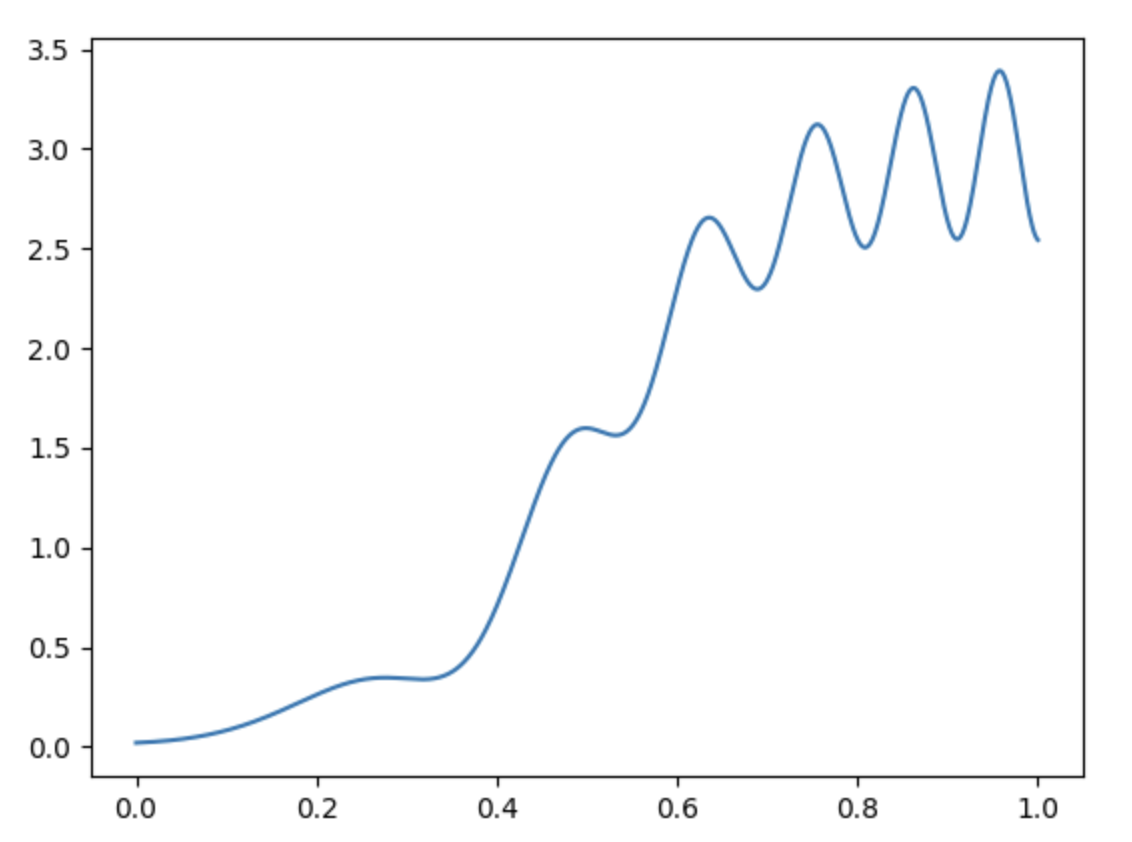
\includegraphics[width=\linewidth]{figures/CART0.png}
    \end{subfigure}\hfill%
    \begin{subfigure}[t]{0.32\textwidth}
        \centering
        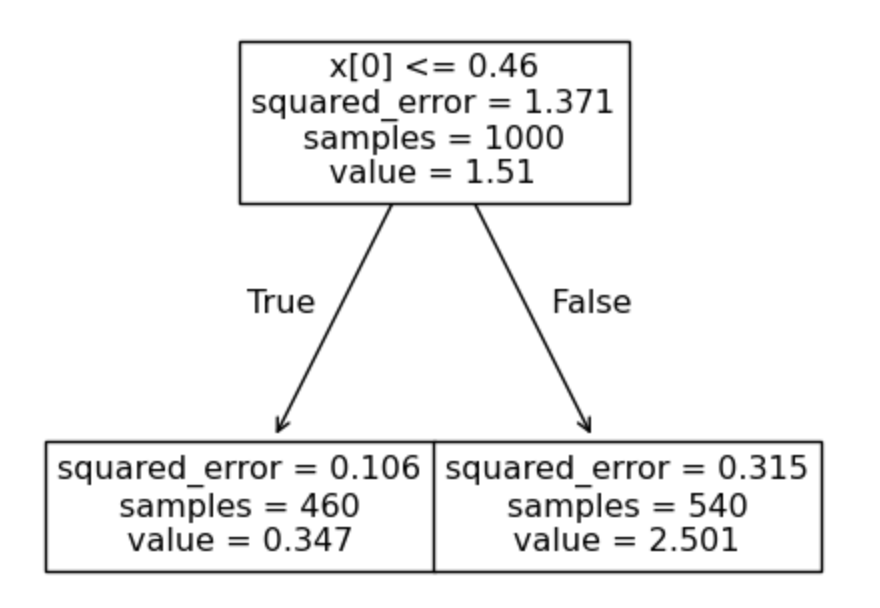
\includegraphics[width=\linewidth]{figures/TREE.png}
    \end{subfigure}\hfill%
    \begin{subfigure}[t]{0.32\textwidth}
        \centering
        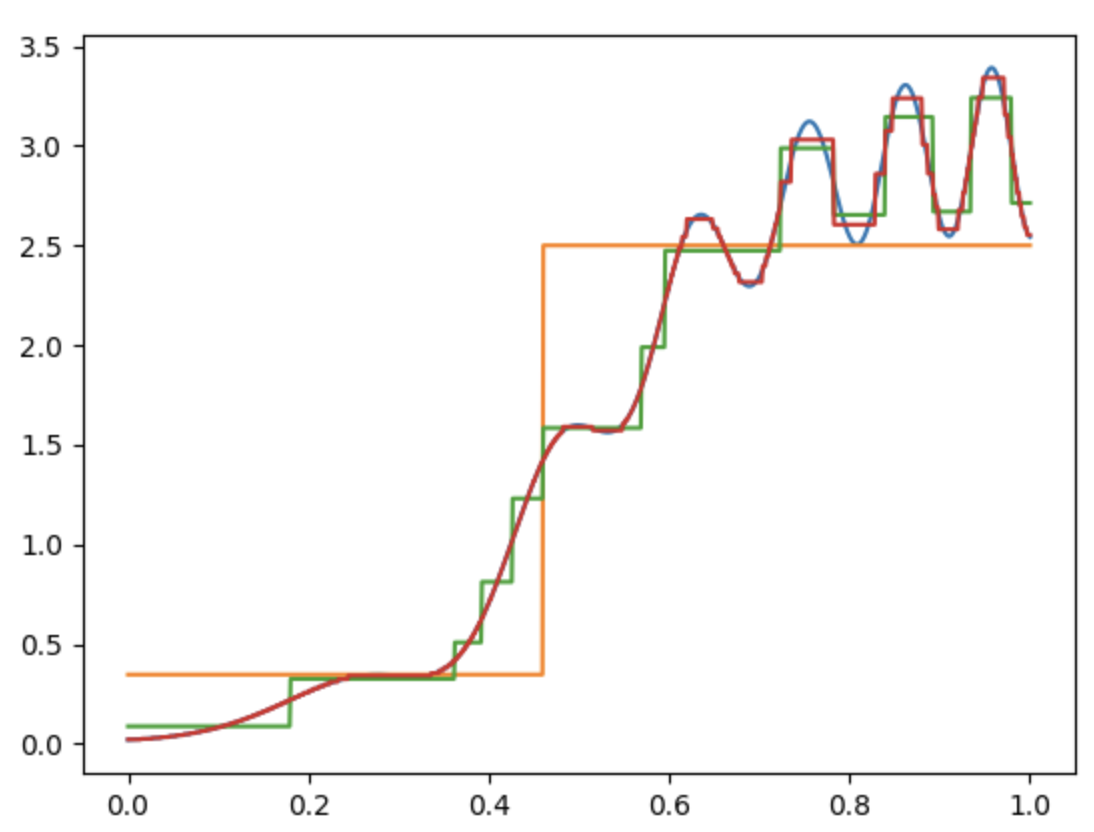
\includegraphics[width=\linewidth]{figures/CART.png}
    \end{subfigure}
    \caption{Classification and Regression Trees}
    \label{fig:cart}
\end{figure}
Classification and Regression Trees (CART) is a tree-based method that recursively splits the data into two groups based on feature values, producing a model that can predict either a category or a numerical value.

In order to choose a more optimal tree, we ``trim'' the tree back by regularizing the size of the tree. Given a starting tree $T$ and a cost complexity parameter $\alpha$, we find the subtree that minimizes
\begin{equation}
    \text{Cost complexity}\,(T') = \sum_{t \in T'} \sum_{n \in t} (y_n - \hat{y}_t)^2 + \alpha |T'|,
\end{equation}
where $t \in T'$ means $t$ is a leaf node of $T'$, $n \in t$ means $\mathbf{x}_n$ is assigned to leaf node $t$, and $|T'|$ counts the number of leaf nodes.

\subsubsection{Bootstrapping}
Let $Y_1, \ldots, Y_N$ be i.i.d.\ observations from an unknown
distribution $F$, and let $\hat{\mu} = s(\boldsymbol{Y})$ be an
estimator of a parameter $\mu$. The \emph{bootstrap} approximates
the sampling distribution of $\hat{\mu}$ by replacing $F$ with the
empirical distribution
\[
  \hat{F}(y) \;=\; \frac{1}{N}\sum_{i=1}^{N} \mathbb{I}(Y_i \le y),
\]
and resampling from the data itself. For $b = 1, \ldots, R$, draw
$\boldsymbol{Y}^{*b} = (Y_1^{*b}, \ldots, Y_N^{*b})$ \textbf{with
replacement} from $\{Y_1, \ldots, Y_N\}$ and compute the bootstrap
replicate $\hat{\mu}^{*b} = s(\boldsymbol{Y}^{*b})$. The empirical
distribution of $\{\hat{\mu}^{*1}, \ldots, \hat{\mu}^{*R}\}$ then
serves as a proxy for the sampling distribution of $\hat{\mu}$.
\begin{rem}
    Bootstrapping's power is
    computational rather than informational: it does not see more than the data, but it extracts what closed-form derivations would discard.
\end{rem}



\subsubsection{Bagging}
Suppose we're using squared error loss, and we have a learner that is
approximately \textbf{unbiased but high variance}. That is, for a particular
fixed $x$, we have $\hat{f}(x; \mathcal{D})$, where $\hat{f}(\cdot; \mathcal{D})$
depends on the training data $\mathcal{D}$, which satisfies
\[
\mathbb{E}_{\mathcal{D}}\left[\hat{f}(x; \mathcal{D})\right] \approx f^*(x)
\quad \text{and} \quad
\mathrm{Var}_{\mathcal{D}}\left(\hat{f}(x; \mathcal{D})\right) \text{ is large.}
\]
Here, $\mathbb{E}\left[y \mid x\right] = f^*(x)$ is the best possible
prediction we could make.

One might think of deep regression trees as being a possible example.
Intuitively, one might expect such a predictor to be over-fitting the
particular dataset at hand.

Recall that we showed earlier that the expected squared error decomposes into
\[
\mathbb{E}_{\mathcal{D}}\left[(\hat{f}(x; \mathcal{D}) - f^*(x))^2\right]
= \underbrace{\mathbb{E}_{\mathcal{D}}\left[\left(\hat{f}(x; \mathcal{D})
- \mathbb{E}_{\mathcal{D}}\left[\hat{f}(x; \mathcal{D})\right]\right)^2\right]}_{\text{Variance}}
+ \underbrace{\left(\mathbb{E}_{\mathcal{D}}\left[\hat{f}(x; \mathcal{D})\right]
- f^*(x)\right)^2}_{\text{Bias}}.
\]

The variance only increases the expected squared error, so if we could
get a lower-variance estimator without changing the bias, we'd improve
our loss. Ideally, we might imagine getting $B$ different, new datasets
$\mathcal{D}_1, \ldots, \mathcal{D}_B$, and then using
\[
\hat{f}_{\text{Ideal}}(x) = \frac{1}{B} \sum_{b=1}^{B} \hat{f}(x; \mathcal{D}_b)
\approx \mathbb{E}_{\mathcal{D}}\left[\hat{f}(x; \mathcal{D})\right].
\]

Of course, if we could actually do this, we should just combine the
datasets into one giant dataset. But this idea motivates the feasible
``bagging'' estimator:
\[
\hat{f}_{\text{Bagging}}(x) = \frac{1}{B} \sum_{b=1}^{B} \hat{f}(x; \mathcal{D}_b^*),
\]
where $\mathcal{D}_b^*$ is a \emph{bootstrap} sample from the original
dataset. The bootstrap distribution is a random distribution
\emph{conditional on the original dataset} $\mathcal{D}$, with probability
distribution
\[
\mathbb{P}\left((x_n^*, y_n^*) = (x_n, y_n)\right) = \frac{1}{N}
\quad \text{for} \quad n = 1, \ldots, N.
\]

The problem is, of course, that bootstrap draws are not draws from
$\mathcal{D}$. Why does bagging work? In my opinion, the theory is not
very clear, but it appears in practice that bagging tends to improve
highly variable and expressive estimators, but can make less variable
estimators worse.

\subsubsection{Boosting}
\begin{algorithm}
\caption{Forward Stagewise Additive Modeling}
\begin{algorithmic}[1]
  \State Initialize $\hat{f}_0(\cdot) = 0$.
  \For{$m = 1, \ldots, M$}
    \State Compute
      \[
        \hat{\theta}_m, \hat{\phi}_m
        \;:=\; \operatorname*{argmin}_{\theta, \phi}
        \frac{1}{N}\sum_{n=1}^{N}
        \mathcal{L}\!\left(\hat{f}_{m-1}(\boldsymbol{x}_n)
        + \theta\phi(\boldsymbol{x}_n),\, y_n\right).
      \]
    \State Set $\hat{f}_m(\cdot) = \hat{f}_{m-1}(\cdot)
      + \hat{\theta}_m \hat{\phi}_m(\cdot)$.
  \EndFor
  \State \Return $\hat{f}_M(\cdot) = \sum_{m=1}^{M}
    \hat{\theta}_m \hat{\phi}_m(\cdot)$.
\end{algorithmic}
\end{algorithm}
For boosting, we first find the $\hat{f}_1(\cdot)$ that best
predicts $y_n$, then the one that makes the biggest improvement when
added to $\hat{f}_1(\cdot)$, and so on. Note that at each step all we
need to be able to do is make a \emph{small improvement}, since over
$M$ steps these small improvements accumulate. For example, we might
take $\hat{\phi}_m(\cdot)$ to simply be a ``stump'': a regression
tree with a single split. In this sense, boosting can improve on
\textbf{high-biased estimators} by adding up a large number of them in an
\textbf{increasingly expressive} way.

\subsection{Cross-Validation}
\subsubsection{Cross-Validation}
We spend some time developing theory to control the generalization
error, $\hat{\mathcal{L}}(\hat{f}) - \mathcal{L}(\hat{f})$. In
practice, however, this theory is not useful because we cannot
actually compute the complexity. More importantly, the worst-case
bounds we computed appear in practice to be \emph{too loose} and may
suggest bad advice (see, e.g., Belkin et al.\ (2019)). In practice,
we most often \emph{estimate} the risk $\mathcal{L}(\hat{f})$ using
held-out data.

Recall that the estimator
$\hat{\mathcal{L}}(\hat{f}) = \frac{1}{N}\sum_{n=1}^{N}
\mathcal{L}(\hat{f}(\boldsymbol{x}_n), y_n)$ is not considered a
reliable estimator of $\mathcal{L}(\hat{f})$ because $\hat{f}$ is
not independent of $(\boldsymbol{x}_n, y_n)$. But suppose we have
an actual new dataset,
$\mathcal{D}_{\text{new}} = ((\boldsymbol{x}_1, y_1), \ldots,
(\boldsymbol{x}_M, y_M))$. Then we could just estimate:
\[
  \hat{\mathcal{L}}_{\text{new}}(\hat{f})
  \;\approx\; \frac{1}{M}\sum_{m=1}^{M}
  \mathcal{L}(\hat{f}(\boldsymbol{x}_m), y_m).
\]
This \emph{is} a consistent estimate of $\mathcal{L}(\hat{f})$ since
we did not use $\mathcal{D}_{\text{new}}$ to train $\hat{f}$, and so
$\hat{f}$ is independent of $\boldsymbol{x}_m, y_m$.

One might ask, if you had $\mathcal{D}_{\text{new}}$, why didn't you
just use it to train $\hat{f}$? Conversely, you might imagine taking
the data you do have, and splitting it (randomly) into a ``training
set'' $\mathcal{D}_{\text{train}}$ and a ``test set''
$\mathcal{D}_{\text{test}}$, using only $\mathcal{D}_{\text{train}}$
to compute $\hat{f}$, and $\mathcal{D}_{\text{test}}$ to estimate
$\hat{\mathcal{L}}_{\text{test}}(\hat{f})$ using the above formula.
There are costs and benefits to doing this:
\begin{itemize}
  \item You have less data to train $\hat{f}$.
  \item You have a good estimate of $\mathcal{L}(\hat{f})$.
\end{itemize}
Putting more data in $\mathcal{D}_{\text{train}}$ ameliorates the
first cost, at the risk of making your estimate of
$\mathcal{L}(\hat{f})$ worse.

A clever way to use nearly all the data to compute $\hat{f}$ and
still get a reasonable test set error is to \emph{repeat} the above
procedure many times, each time with a different test set.

As an extreme, let $\hat{f}_{-n}$ denote an estimate of $\hat{f}$
with the $n$-th datapoint removed. Since you have removed only one
datapoint, we might hope that $\hat{f}_{-n} \approx \hat{f}$, so we
have paid little estimation cost. Of course, the estimate
\[
  \hat{\mathcal{L}}_{\text{test}}(\hat{f}_{-n})
  \;=\; \mathcal{L}(\hat{f}_{-n}(\boldsymbol{x}_n), y_n)
\]
uses a single datapoint, and so is very variable, if nearly
unbiased. However, we can do this for \emph{each} datapoint and
average the results to reduce the variance of the test error
estimate. This is called the ``leave-one-out CV estimator,'' or
LOO-CV:
\[
  \hat{\mathcal{L}}_{\text{LOO}}
  \;:=\; \frac{1}{N}\sum_{n=1}^{N}
  \mathcal{L}(\hat{f}_{-n}(\boldsymbol{x}_n), y_n).
\]
Of course, you can do the same thing leaving two points out, or
three, or so on, giving ``leave-$k$-out CV'' estimators. In the
extreme where you leave a fraction $N/K$ points out, you get
``$K$-fold'' CV estimators.

How many should you leave out? There seems to be a striking lack of
useful theory. The rules of thumb are:
\begin{itemize}
  \item By leaving out more datapoints you ``bias'' your estimate
        if your estimate of $\hat{f}$ depends strongly on how many
        datapoints you have.
  \item By leaving out more datapoints you reduce the ``variance''
        of your estimate of $\mathcal{L}(\hat{f})$ by making the
        test set larger.
\end{itemize}
So there appears to be a sort of meta-bias-variance tradeoff in the
estimation of $\mathcal{L}(\hat{f})$. Common practice is five- or
ten-fold cross-validation.

\subsubsection{Influence Function}
The influence function estimates how the model parameters (or predictions)
change when a training sample is slightly perturbed, without retraining.

Let the parameters $\hat\theta$ minimize the empirical risk
$\hat\theta = \arg\min_{\theta} \frac{1}{n}\sum_{i=1}^{n} \mathcal{L}(z_i,\theta)$.
Now upweight the $i$-th sample by a small $\epsilon$, giving the perturbed
optimizer
\[
  \hat\theta_{\epsilon,z_i}
  = \arg\min_{\theta}\ \frac{1}{n}\sum_{j=1}^{n} \mathcal{L}(z_j,\theta)+\epsilon\,\mathcal{L}(z_i,\theta).
\]

Differentiating with respect to $\epsilon$ at $\epsilon=0$ yields the influence
of this sample on the parameters,
\[
  \mathcal{I}_{\text{params}}(z_i)
  = \left.\frac{d\hat\theta_{\epsilon,z_i}}{d\epsilon}\right|_{\epsilon=0}
  = -\,H_{\hat\theta}^{-1}\,\nabla_\theta \mathcal{L}(z_i,\hat\theta),
\]
where $H_{\hat\theta}=\frac{1}{n}\sum_{i=1}^{n}\nabla_\theta^2 \mathcal{L}(z_i,\hat\theta)$
is the Hessian. Since deleting a sample corresponds to $\epsilon=-\tfrac{1}{n}$,
the parameter change from removal is approximately
$-\tfrac{1}{n}\,\mathcal{I}_{\text{params}}(z_i)$.

By the chain rule, the influence of a training sample $z$ on the loss at a test
point $z_{\text{test}}$ is
\[
  \mathcal{I}(z,z_{\text{test}})
  = -\,\nabla_\theta \mathcal{L}(z_{\text{test}},\hat\theta)^{\top}\,
       H_{\hat\theta}^{-1}\,
       \nabla_\theta \mathcal{L}(z,\hat\theta).
\]
Intuitively, the more aligned the two gradients are after weighting by
$H_{\hat\theta}^{-1}$, the more the training sample $z$ helps that prediction.

\subsection{Time Series}
\todo

\newpage
\part{Chapter 2: High-Dimensional Statistics}
\newpage
\section{Classic Statistics Model 1 -- Linear Regression, Bias-Variance Decomposition, LASSO, Feature Engineering}
\newpage
\section{Classical Statistics Model 2 -- SVM, Random Forest, Kernel Method, Bagging, Boosting, Time Series}
\newpage
\section{From Traditional Statistics to Modern Statistics: Compressed Sensing, Sparse Representation, Robust PCA, Matrix Recovery}
\newpage
\section{Random Matrix Theory}
In addition to non-asymptotic results, we will need asymptotic analysis, which is more delicate. The section is organized as follows: 
\begin{enumerate}
    \item Density of eigenvalues in classical ensembles of random matrices
    \item Semi-Circle Law and Marchenko–Pastur Law
    \item BBP Transition
    \item CLT for Eigenvalues
    \item Spectrum Separation
    \item Replica Method
\end{enumerate}

This section mainly follows STATC206B (UC Berkeley, taught by Vadim Gorin) and STAT260 (UC Berkeley, taught by Song Mei, 2021). I also refered to the book~\cite{bai2010spectral}.

\subsection{Density of Eigenvalues in Classical Ensembles of Random Matrices}

We begin our tour from an important type of matrix G$\beta$E ($\beta=1,2,4$). Let $X$ be $N\times N$ matrix with i.i.d. entries: 
\[
\begin{cases}
    a) \normalg \\
    b) \normalg + i\normalg \\
    c) \normalg + i\normalg + j\normalg + k\normalg
\end{cases}
\]
Set $M = \frac{1}{2}(X+X^*)$, and we have the main theorem.
\begin{thm}[Density of Eigenvalues]
    Let the eigenvalues of $M$ be $\lambda_1\ge \lambda_2\ge ...\ge \lambda_N$, and they have density
    \[
    \frac{1}{Z} \prod_{i<j}|\lambda_j-\lambda_i|^\beta \cdot \prod_{i=1}^N\exp(-\frac{\lambda_i^2}{2}) \dd \lambda_{1}...\dd \lambda_{N}.
    \]
    where $\beta = 1,2,4$ for a), b), c) and 
    \[
    Z = \frac{(2\pi)^{N/2}}{N!} \prod_{j=0}^N \frac{\Gamma(1+(j+1)\beta/2)}{\Gamma(1+\beta/2)}
    \]
    is the partition function (normalization factor).
\end{thm}
\begin{proof}
    We prove $\beta = 1$ here and leave $\beta = 2$ to the homework.

    \paragraph{Step 1}  Claim density of $M = \frac{1}{2}(X+X^*) \sim \exp(-\frac{1}{2}\tr(M^2))$.

    Indeed, 
    \[
    \tr(M^2) = \sum_{i,j} m_{ij}^2 = \sum_{i=1}^N \underbrace{x_{ii}^2}_{\mathcal{N}(0,1)} + \frac{1}{2}\sum_{i<j} \underbrace{(x_{ij}+x_{ji})^2}_{\mathcal{N}(0,2)}
    \]
    implies that the density of $M\propto \exp(-\frac{1}{2}\tr(M^2))$

    \paragraph{Step 2}  We can calculate that $\exp(-\frac{1}{2}\tr(M^2)) = \prod_{i=1}^N \exp(-\frac{\lambda_i^2}{2})$.

    We derive it immediately by diagonalizing the the matrix $M$.

    \paragraph{Step 3}  Each symmetric matrix is determined by its eigenvalues and eigenvectors, i.e. there exists an almost bijection $\pi$
    \[
    \pi: \underbrace{\mathcal{W}_N}_{\lambda_1<\lambda_2<...<\lambda_N} \times \underbrace{O(N)}_{\text{Orthogonal Bases}} \to \underbrace{\mathcal{H}_N}_{\text{Symmetric Matrix}}
    \]
    We say "almost" because indeed the map is not injective: we can multiply the eigenvalue by $\pm 1$. In other words, if the eigenvalues are unique, $\pi^{-1}(M)$ has exactly $2^N$ elements.

    Now we give the key proposition of the proof.
    \begin{prop}[Jacobian]
        Consider the map $\pi: (\Lambda, O) \mapsto B$, where $\pi((\Lambda, O)) = O\Lambda O^*$. Then the Jocobian of the map is $\prod_{i<j} |\lambda_j-\lambda_i|$.
    \end{prop}
    \begin{rem}
        It is an important technique to transform an intractable density calculation into a tractable one and a Jocobian.
    \end{rem}
    \begin{proof}
        It is sufficient to calculate by taking $O = \Id$, as when we transform $O$ to $A\cdot O$ (where $A$ is orthogonal), the \textbf{uniform measure} on $O(N)$ and the Lebesgue measure on $\mathcal{H}(N)$ remain unchanged.

        Then we take $O = \exp(B) = \Id + B + ...$ and we can deduce that $B + B^* = 0$ as $OO^* = \Id$. Then the map $\pi$ can be written as
        \begin{align*}
        \left((\lambda_1,...,\lambda_N), \exp(B)\right)
        &\mapsto \exp(B)
        \begin{pmatrix}
        \lambda_1 & 0 & 0 & \cdots & 0 \\
        0 & \lambda_2 & 0 & \cdots & 0 \\
        0 & 0 & \lambda_3 & \cdots & 0 \\
        \vdots & \vdots & \vdots & \ddots & \vdots \\
        0 & 0 & 0 & \cdots & \lambda_n
        \end{pmatrix}
        \exp(-B)\\
        &\mapsto (\Id+B)
        \begin{pmatrix}
        \lambda_1 & 0 & 0 & \cdots & 0 \\
        0 & \lambda_2 & 0 & \cdots & 0 \\
        0 & 0 & \lambda_3 & \cdots & 0 \\
        \vdots & \vdots & \vdots & \ddots & \vdots \\
        0 & 0 & 0 & \cdots & \lambda_n
        \end{pmatrix}
        (Id-B) + o(B)\\
        &\mapsto 
        \begin{pmatrix}
        \lambda_1 & 0 & 0 & \cdots & 0 \\
        0 & \lambda_2 & 0 & \cdots & 0 \\
        0 & 0 & \lambda_3 & \cdots & 0 \\
        \vdots & \vdots & \vdots & \ddots & \vdots \\
        0 & 0 & 0 & \cdots & \lambda_n
        \end{pmatrix}\\
        &+
        \begin{pmatrix}
        0 & b_{12}(\lambda_2 - \lambda_1) & b_{13}(\lambda_3 - \lambda_1) & \cdots & b_{1n}(\lambda_n - \lambda_1) \\
        b_{21}(\lambda_1 - \lambda_2) & 0 & b_{23}(\lambda_3 - \lambda_2) & \cdots & b_{2n}(\lambda_n - \lambda_2) \\
        b_{31}(\lambda_1 - \lambda_3) & b_{32}(\lambda_2 - \lambda_3) & 0 & \cdots & b_{3n}(\lambda_n - \lambda_3) \\
        \vdots & \vdots & \vdots & \ddots & \vdots \\
        b_{n1}(\lambda_1 - \lambda_n) & b_{n2}(\lambda_2 - \lambda_n) & b_{n3}(\lambda_3 - \lambda_n) & \cdots & 0
        \end{pmatrix}
        + o(B)
        \end{align*}
        As $B$ has only $\frac{n(n-1)}{2}$ free parameter, so the Jacobian of the map is $\prod_{i<j}|\lambda_j-\lambda_i|$.
    \end{proof}
    
    \paragraph{Step 4}  We now calculate $Z$:
    \begin{align*}
        Z = \int_{\mathbb{R}^N} \prod_{i<j}|\lambda_j-\lambda_i|^\beta \cdot \prod_{i=1}^N\exp(-\frac{\lambda_i^2}{2}) \dd \lambda_{1}...\dd \lambda_{N} = 
        \frac{(2\pi)^{N/2}}{N!} \prod_{j=0}^N \frac{\Gamma(1+(j+1)\beta/2)}{\Gamma(1+\beta/2)}
    \end{align*}
\end{proof}

\subsection{Semi-Circle Law and Marchenko–Pastur Law}
\subsubsection{Trace Calculation}
\begin{thm}[Tridiagonal Matrix Equivalent]
    Consider the real symmetric tridiagonal matrix
    \[
    T_{\beta} = 
    \begin{pmatrix}
    \cN(0,1) & \frac{1}{\sqrt{2}}\chi_{\beta(n-1)} & \cdots & 0 \\
    \frac{1}{\sqrt{2}}\chi_{\beta(n-1)} & \cN(0,1) & \cdots & 0 \\
    \vdots & \vdots & \ddots & \vdots \\
    0 & 0 & \cdots & \cN(0,1)
    \end{pmatrix}
    \]
    where the second diagonal entries are $\chi_{\beta(n-1)}, \chi_{\beta(n-2)},... \chi_{\beta}$.
    $\chi_k = \sqrt{\chi_k^2} = \sqrt{\sum_{i=1}^k \cN(0,1)^2}$, whose density is
    \[
    \frac{1}{2^{\frac{k}{2}-1}\Gamma(\frac{k}{2})}x^{k-1}e^{-\frac{x^2}{2}}.
    \]
    Then the eigenvalues of $T_\beta$ have the same distribution of $G\beta E$.
\end{thm}

\begin{proof}
    We present for $\beta = 1$. By linear algebra, we can choose an orthogonal matrix $U_1$, and transform the matrix $M$ to $U_1MU_1^\top$, whose the first row is 
    \[
    (x_{11}, \sqrt{\sum_{k=2}^n x_{ik}^2}, 0,...,0).
    \]
    Note that the eigenvalues do not change after the transformation.
    
    We can inductively do the same operation on the rest sub-matrix.
\end{proof}

\begin{cor}
    For $\beta = 1, 2, 4$, the law of eigenvalues $\sim \prod_{i<j} (x_i-x_j)^\beta \prod_{i=1}^N\exp(-\frac{x_i^2}{2})$.
\end{cor}

\begin{thm}
    In fact, the corollary is true for any $\beta>0$.
\end{thm}

Now we begin to prove the semi-circle law. First we give the key result of trace calculation.
\begin{thm}[Semi-Circle Law]
    For each $k>0, \beta>0$, we have
    \[
    \frac{1}{N^{\frac{k}{2}+1}} \tr(T_\beta^k)=
    \frac{1}{N^{\frac{k}{2}+1}}\sum_{i=1}^N X_i^k
    \xrightarrow{N\to \infty, \text{in probability}} 
    \begin{cases}
        0&, \quad \text{k is odd}; \\
        (\frac{\beta}{2})^k \Cat_{\frac{k}{2}}&, 
        \quad \text{k is even}.
    \end{cases}
    \]
    where $\Cat_k$ is the k-the catalan number defined as
    \[
    \Cat_k = \frac{1}{k+1} \binom{2k}{k}.
    \]
\end{thm}

\begin{proof}
    By SLLN, we have
    \begin{align*}
        &\lim_{N\to \infty} \frac{\chi_{\beta(N-1)}}{\sqrt{2N}} = \sqrt{\frac{\beta}{2}},\\
        &\lim_{N\to \infty} \frac{\chi_{\beta(N-\alpha N)}}{\sqrt{2N}} = \sqrt{\frac{\beta(1-\alpha)}{2}}.
    \end{align*}
    So by the definition of the trace, we have
    \begin{align*}
    \tr \ \left(\frac{T_\beta}{\sqrt{N}}\right)^k 
    &= \sum_{m=1}^N \sum_{\substack{\text{k-step paths} \\ \text{from } m \text{ to } m}} 
    \left(\ \textcolor{gray}{ \text{some} 
    \ \frac{\chi_{\beta(N-i)}}{\sqrt{2N}} } \right)
    \left(\ \textcolor{gray}{ \text{some} 
    \ \frac{\mathcal{N}(0,1)}{\sqrt{N}} }\right)\\
    &=\sum_{m=1}^N \left( \# {\text{k-step paths from } m \text{ to } m} \right) \sqrt{\frac{\beta}{2}\left( \frac{N-m}{N} \right)^k} + o(N).
    \end{align*}
    The second equation follows from that if there exists "some $\frac{\mathcal{N}(0,1)}{\sqrt{N}}$", the term vanishes. 
    When $2 \nmid k$, $\# {\text{k-step paths from } m \text{ to } m}$ is zero.
    When $2\mid k$, $\# {\text{k-step paths from } m \text{ to } m} = \binom{k}{\frac{k}{2}}$. Approximate the summation by integration and we have
    \[
    \frac{1}{N} \tr \ \left(\frac{T_\beta}{\sqrt{N}}\right)^k \to \binom{k}{\frac{k}{2}} \left(\frac{\beta}{2}\right)^{\frac{k}{2}} \int_0^1 x^{\frac{k}{2}}\dd x = \Cat_{\frac{k}{2}} \left(\frac{\beta}{2}\right)^{\frac{k}{2}}
    \]
\end{proof}

Now we introduce the semi-circle distribution.
\begin{defn}[Wiegner Semi-Circle Distribution]
    The density of the distribution is
    \[
    \mu(x) = \frac{1}{2\pi} \sqrt{4-x^2}.
    \]
\end{defn}

We use moment method to recover the proof and give the definition.
\begin{cor}[Moment Analysis]
    Let $m_k$ are moments of $T_\beta$ and we have
    \[
    m_u = \begin{cases}
        0&,\quad u \text{ is odd}; \\
        \frac{1}{\frac{u}{2}+1}\binom{u}{\frac{u}{2}} &,\quad u \text{ is even}.
    \end{cases}
    \]
\end{cor}

\begin{thm}[Moment of Semi-Circle Distribution]
    \label{thm:scl}
    $m_k$ are moments of semi-circle law and
    \[
    m_k = \int_{-2}^2 \mu(x) x^k \dd x.
    \]
\end{thm}

\begin{proof}{(Method I)}
    We just calculate
    \[
    m_k = \int \frac{1}{\sqrt{2\pi}} \sqrt{4-x^2}x^k \dd x.
    \]
    Let $x = 2\cos\theta$, and by inductive calculation, we derive the results.
\end{proof}

However, we are not satisfied for the calculation is not so intuitive. We then introduce another proof.

\begin{proof}{(Method II)}
Introduce generating function: 
\[
G(z) = \sum_{k=0}^\infty m_k z^{-k-1},
\]
$m_0 =1$. By classical results, we have
\[
\sum_{n=0}^\infty \Cat_n x^n = \frac{1-\sqrt{1-4x}}{2x} =: C(x).
\]
Now we can derive the expression of $G(z)$ using $C(x)$.
\[
    G(z) = \sum_{k=0}^\infty m_k z^{-k-1} = \sum_{l=0}^\infty \Cat_l z^{-2l-1} = \frac{z-\sqrt{z^2-4}}{2}.
\]
Next we introduce two propositions.
\begin{prop}[Stieltjes Transform]
    \label{prop:2.8}
    \[
    G(z) = \int \frac{\mu(x)}{z-x} \dd x.
    \]
\end{prop}
\begin{proof}
    By Taylor expansion, we have
    \begin{align*}
    \int \frac{\mu(x)}{z-x} \dd x 
    &= \frac{1}{z} \int \frac{\mu(x)}{1-\frac{x}{z}}\dd x\\
    &= \frac{1}{z}\int \mu(x)\sum_{k=0}^\infty\left( \frac{x}{z}\right)^k\\
    &=\sum_{k=0}^\infty m_k z^{-k-1} \\
    &= G(z)
    \end{align*}
\end{proof}

\begin{prop}
    \label{prop:2.9}
    \[
    \mu(x_0) = -\frac{1}{\pi} \lim_{y_0\to 0^+} \Im (G(x_0+iy_0)).
    \]
\end{prop}
\begin{rem}
    We can just add a perturbation onto the imagine axis and obtain the information of the point.
\end{rem}

\begin{proof}
    By proposition \ref{prop:2.8}, we have
    \begin{align}
        -\frac{1}{\pi}  \Im (G(x_0+iy_0))
        &= -\frac{1}{\pi} \int  \Im \frac{1}{x_0+iy_0-x} \mu(x)\dd x\\
        &= -\frac{1}{\pi} \int \Im \frac{x_0-x-iy_0}{(x-x_0)^2+y_0^2}\mu(x) \dd x\\
        &= \int \frac{1}{\pi} \frac{y_0}{(x-x_0)^2+y_0^2}\mu(x) \dd x.
    \end{align}
    Notice that $\frac{1}{\pi} \frac{y_0}{(x-x_0)^2+y_0^2}$ is a "good" kernel, and thus as $y_0\to 0$
    \[
    \int \frac{1}{\pi} \frac{y_0}{(x-x_0)^2+y_0^2}\mu(x) \dd x \to \mu(x_0).
    \]
\end{proof}
Return to the Theorem \ref{thm:scl}, by proposition \ref{prop:2.9}
\[
\mu(x_0) = -\frac{1}{\pi} \lim_{y\to 0^+} \Im \left( \frac{1}{2}\left[(x+iy) - \sqrt{(x+iy)^2 - 4)}\right]
\right) = \begin{cases}
    0  &, \quad |x|>2;\\
    \frac{\sqrt{4-x^2}}{2\pi} &,\quad |x|\le 2.
\end{cases}
\]
\end{proof}

Now we are prepared to formally state and prove the semi-circle law.
\begin{thm}[Semi-Circle Law]
    Let $\lambda_1 < ... <\lambda_N$ be eigenvalues of G$\beta$E. Set $x_i = \lambda_i\sqrt{\frac{2}{\beta N}}$ and let $\mu_N$ be their empirical measure: $\mu_N = \frac{1}{\sqrt{N}}\sum_{i=1}^N \delta_{x_i}$. Then
    \[
    \lim_{N\to \infty} \mu_N = \frac{1}{2\pi} \sqrt{4-x^2} \mathbbm{1}_{|x|\le 2} = \mu_{\text{circle}}(x)
    \]
    weakly in probability, which means $\forall$ bounded continuous function $f(x)$
    \[
    \lim_{N\to \infty} \int_{\RR} f(x)\mu_N(x) = \int_{\RR} f(x)\mu(x) \dd x.
    \]
\end{thm}

\begin{proof}
    We prove the result in four steps.
    \paragraph{Step 1}  The results hold for $f(x) = x^k$.
    
    \paragraph{Step 2}  The results hold for any polynomials. 
    
    \paragraph{Step 3}  Take $L>2$, the results hold for $f(x) = \mathbbm{1}_{|x|>L} x^k$.
    We have
    \begin{align*}
        \left|\int f(x)\mu_N(\dd x)\right| 
        &= \left|\int x^k\mu_N(\dd x)\right|\\
        &\le L^{-2m} \int_{|x|\ge L} x^{2k+2m}\mu_N(\dd x)\\
        &\to L^{-2m} \int x^{2k+2m} \mu(\dd x)\\
        &\le L^{-2m} 2^{2k+2m} = 2^{2k} \left(\frac{2}{L}\right)^m \to 0. 
    \end{align*}
    
    \paragraph{Step 4}  By step 3, we can restrict the support set of $f$ on a compact set, i.e. $[-4, 4]$. Apply the Weierstrass theorem and we get the proof.
\end{proof}

At last, we give three generalizations of the semi-circle law. Next theorem tells us the gaussian assumption of the semi-circle law is not neccessary.
\begin{thm}[Generalization]
    Let $z_{ij}, i<j$ be i.i.d. random variables with finite moments. $\EE z_{ij} = 0$ and $\EE z_{ij}^2 = \frac{1}{2}$. Let $Y_i$ be i.i.d. with finite moments. Then the semi-circle law still holds for the matrix with entries $Y_i$ and $z_{ij}$.
\end{thm}

\subsubsection{Marchenko–Pastur Law}
Now we consider the case where the matrix is not square.
Let $X$ be an $N\times S$ random matrix whose elements are Gaussian with parameter $\beta > 0$ (different form according to $\beta$).
Assume that $N, S\to\infty$ in such a way that $N/S \to \gamma^2 \in (0,1)$.
Let $\lambda_1, \lambda_2,\ldots, \lambda_N$ denote the eigenvalues of $\frac{1}{S}XX^*$, and define the empirical spectral measure
\[
\rho^N = \frac{1}{N}\sum_{i=1}^N \delta_{\lambda_i}.
\]
 
\begin{thm}[Marchenko--Pastur Law]
As $N\to\infty$ (with $N/S\to \gamma^2\in(0,1)$), the empirical spectral measure $\rho^N$ converges weakly, in probability, to the Marchenko--Pastur distribution $\mu_{\mathrm{MP}}$ with density
\[
\frac{\dd\mu_{\mathrm{MP}}}{\dd x}(x)
= \frac{1}{2\pi\beta\gamma^2}\,
\frac{\sqrt{(\lambda_+ - x)(x-\lambda_-)}}{x}\,
\mathbf{1}_{[\lambda_-,\,\lambda_+]}(x),
\]
where
\[
\lambda_+ = \beta(1+\gamma)^2, \qquad
\lambda_- = \beta(1-\gamma)^2.
\]
\end{thm}

\begin{proof} We calculate the moments for $\rho^N$ and $\mu_{\mathrm{MP}}$ separately
    \paragraph{Step 1} We claim that
    \[
    \lim_{N,S\to \infty} \frac{1}{NS^k}\tr[(XX^*)^k] = \beta^k \sum_{r=0}^{k-1} \frac{\gamma^{2r}}{r+1} \binom{k}{r} \binom{k-1}{r}.
    \]

    Notice that as $S\to \infty$
    \[
    \frac{\chi_{aS}}{\sqrt{S}} \to \sqrt{a},
    \]
    we have
    \begin{align*}
        \operatorname{LHS} &= \lim_{S,N\to\infty}\frac{1}{NS^k} \sum_{m=1}^N\sum_{\substack{\text{k-step paths} \\ \text{from } m \text{ to } m}} (\text{diagonal entries})(\text{sub-diagonal entries})\\
        &= \lim_{S,N\to \infty} \frac{1}{NS^k} \sum_{m=1}^N \sum_{i=0}^{[k/2]} \left(
        \chi_{\beta(N-m)}\chi_{\beta(S-m+1)}
        \right)^{2i}\chi_{S+N-2m-2}^{2(k-2i)} \binom{k}{2i}\binom{2i}{i}
    \end{align*}
    By replacing $\chi$ by its limit, we have
    \[
    \frac{\chi_{\beta(N-m)}\chi_{\beta(S-m+1)}}{S} \to \beta \sqrt{(\gamma^2-\frac{m}{S})(1-\frac{m}{S})}
    \]
    \[
    \frac{\chi^2_{\beta(S+N-2m+2)}}{S} \to \beta(1+\gamma^2 - 2\frac{m}{S})
    \]
    Then we approximate the sum by integral
    \begin{align*}
    \operatorname{LHS} 
    &= \frac{\beta^k}{\gamma^2} \sum_{i=0}^{[k/2]} \binom{k}{2i}\binom{2i}{i} \int_0^{\gamma^2} (\gamma^2-t)^i(1-t)^i (1+\gamma^2-2t)^{k-2i}\dd t\\
    &=\frac{\beta^k}{\gamma^2} \sum_{i=0}^{[k/2]} \binom{k}{2i}\binom{2i}{i} \int_0^{\gamma^2} u^i(1-\gamma^2+u)^i (1-\gamma^2+2u)^{k-2i}\dd u
    \end{align*}
    We claim that
    \[
    \frac{1}{\gamma^2}\sum_{i=0}^{[k/2]} \binom{k}{2i}\binom{2i}{i} \int_0^{\gamma^2} u^i(1-\gamma^2+u)^i (1-\gamma^2+2u)^{k-2i}\dd u = \sum_{r=0}^{k-1} \frac{\gamma^{2r}}{r+1} \binom{k}{r} \binom{k-1}{r}.
    \]
    and we obtain the proof.

    The proof of the claim: 
    Denote the left hand side as A. First, we observe that
    \begin{equation}
        \label{eq:key}
        \operatorname{A} = \text{The sum of coefficients of all the }x^iy^i \text{ in} \int_{0}^{\gamma^2} [xu+y(1-\gamma^2 +u)+(1-\gamma^2+2u)]^k\dd u
    \end{equation}
    Denote B as the integral of (\ref{eq:key})
    \begin{align*}
        B &= \frac{1}{\gamma^2}\frac{[(x+1)\gamma^2+(y+1)]^{k+1} - [(y+1)(1-\gamma^2)]^{k+1}}{(x+y+2)(k+1)}\\
        &=\frac{1}{k+1}\sum_{l=0}^k [(y+1)(1-\gamma^2)]^l [(x+1)\gamma^2+y+1]^{k-l}.
    \end{align*}
    To calculate the coefficients, we can let $x = \frac{1}{y}$ and calculate the constant coefficient.
    \begin{align*}
        \operatorname{B} &= \frac{1}{k+1} \sum_{l=0}^k [(y+1) (1-\gamma^2)]^l
        \left(\left(\frac{1}{y}+1\right)\gamma^2 + y+1\right)^{k-l}\\
        &=\frac{(y+1)^k}{k+1}
        \sum_{l=0}^k(1-\gamma^2)^l(\frac{1}{y}\gamma^2+1)^{k-l}\\
        &=\frac{(y+1)^k}{k+1} \frac{(\frac{1}{y}\gamma^2+1)^{k+1} - (1-\gamma^2)^{k+1}}
        {\frac{1}{y}\gamma^2 + \gamma^2}\\
        &=\frac{y(y+1)^{k-1}}{(k+1)\gamma^2} \left(\left(\frac{1}{y}\gamma^2+1\right)^{k+1} - (1-\gamma^2)^{k+1}\right)
    \end{align*}
    Then the constant coefficient is
    \[
    \frac{1}{(k+1)\gamma^2} \sum_{r=0}^{k-1} \binom{k-1}{r} \binom{k+1}{r+1} \gamma^{2r+2} = \sum_{r=0}^{k-1} \frac{\gamma^{2r}}{r+1} \binom{k}{r} \binom{k-1}{r}.
    \]
    
    \paragraph{Step 2} We claim that $\lambda_{+} = \beta(1+\gamma)^2$ and $\lambda_{-} = \beta(1-\gamma)^2$.
    
    Define the density of the limit distribution
    \[
    \mu(x) = \frac{1}{2\pi\gamma^2}\frac{\sqrt{(\lambda_{+}-x)(x-\lambda_{-})}}{x} \mathbbm{1}_{[\lambda_{-}, \lambda_{+}]}
    \]
    and $\mu_N = \rho^N$.
    
    The calculation below is inspired by \href{http://ndl.ethernet.edu.et/bitstream/123456789/60805/1/140.pdf}{Zhidong Bai's book}.
    First, we calculate the moment of $\mu(x)$, for $m\ge 1$,
    \begin{align*}
        \EE_{\mu} x^m &= \int x^m \mu(x)\dd x\\
        &= \frac{1}{2\pi\gamma^2}\int x^{m-1} \sqrt{(\lambda_{+}-x)(x-\lambda_{-})} \dd x\\
        &= \frac{1}{2\pi\gamma^2}(2\gamma)^2\int_{-1}^1 (1+\gamma^2+2\gamma u)^{m-1}\sqrt{1-u^2}\dd u
        \\
        &(\text{by setting }x =\beta(1+\gamma^2+2\gamma u))\\
        &= \beta^m\frac{1}{\pi}\sum_{l=0}^{[(m-1)/2]} \binom{m-1}{2l}(1+\gamma^2)^{m-1-2l}
        (4\gamma^2)^l
        \int_{-1}^1 u^{2l}\sqrt{1-u^2}\dd u\\
        &= \beta^m
        \sum_{l=0}^{[(m-1)/2]} \binom{m-1}{2l} 
        \frac{1}{l+1}\binom{2l}{l} (1+\gamma^2)^{m-1-2l} \gamma^{2l}\\
        &= \beta^m\sum_{l=0}^{[(m-1)/2]}\sum_{s=0}^{m-1-l} \frac{(m-1)!}{l!(l+1)!s!(m-1-2l-s)!}\gamma^{2(l+s)}\\
        &=\beta^m \frac{1}{m}\sum_{r=0}^{m-1} \gamma^{2r} \binom{m}{r} \sum_{l=0}^{r\wedge(m-1-r)}\binom{r}{l} \binom{m-r}{m-r-l-1}\\
        &=\beta^m \frac{1}{m}\sum_{r=0}^{m-1}\binom{m}{r}\binom{m}{r+1}\gamma^{2r}\\
        &=\beta^m \sum_{r=0}^{m-1}\frac{1}{r+1}\binom{m}{r}\binom{m-1}{r}\gamma^{2r}.
    \end{align*}

    Next, we notice that
    \[
        \EE_{\mu_N} x^m =\frac{1}{N} \sum_{i=1}^N \lambda_i^N = \frac{1}{N}\tr\left[\left(\frac{XX^*}{S}\right)^m\right]
    \]
    and
    \[
    \lim_{N\to \infty} \frac{1}{N}\tr\left[\left(\frac{XX^*}{S}\right)^m\right] = \beta^m \sum_{r=0}^{m-1}\frac{1}{r+1}\binom{m}{r}\binom{m-1}{r}\gamma^{2r}.
    \]
    So we have
    \[
    \lim_{N\to \infty}\EE_{\mu_N} x^m = \EE_{\mu} x^m.
    \]
    Similar to the proof of semi-circle law, we have $\rho^N$ converges (weakly, in probability) to the Marchenko-Pastur law.
\end{proof}


\subsection{BBP Transition}
In the spiked model $\Sigma = I + \theta\, vv^*$, Baik, Ben Arous, and P\'{e}ch\'{e} (2005) discovered a phase transition for $\lambda_{\max}$ of $\Sigma$. In general form, it is stated as

\begin{thm}[Spiked Random Matrices]
    \label{thm:9.1}
    Let $\lambda_1<\lambda_2<\cdots<\lambda_N$ are $N$ eigenvalues of 
    \[
    C = \sqrt{N}a vv^* +\sqrt{\frac{2}{\beta}}G\beta E,
    \]
    where $\|v\|=1$
    Then there exists $a_{crit}$ such that
    \begin{enumerate}
        \item If $a>a_{crit} = 1$, then 
        \[
        \lim_{N\to\infty} \frac{\lambda_N}{\sqrt{N}} = a+\frac{1}{a} >2.
        \]
        \item If $a<a_{crit}$, then 
        \[
        \lim_{N\to\infty} \frac{\lambda_N}{\sqrt{N}} = 2.
        \]
    \end{enumerate}
\end{thm}
By the theorem, we can easily get
\begin{cor}
    \[
    \hat{a} = \frac{1}{2}\left(
    \frac{\lambda_N}{\sqrt{N}}+\sqrt{\frac{\lambda_N^2}{N}-4}
    \right) \overset{N\to\infty}{\longrightarrow} a.
    \]
\end{cor}
\begin{thm}[Recover $v$]
    \label{thm:9.2}
    In the setting of Theorem \ref{thm:9.1}. Let $\hat{v}$ denote the eigenvector corresponding to $\lambda_N$ and let $\phi$ be the angle between $v$ and $\hat{v}$,
    \[
    \lim_{N\to\infty} \sin\phi = \frac{1}{a} \wedge 1.
    \]
\end{thm}
\begin{proof}
    We prove the results in three steps.
    \paragraph{Step 1} \ $a, \lambda_N$ and $\phi$ are unchanged under orthogonal/unitary transformations of matrix $C$. We do two transformations:
    \begin{itemize}
        \item Rotate $v$ ti be the first basis vector $(1, 0^{N-1})$.
        \item Rotate in the orthogonal complement of $(1, 0^{N-1})$, so that the $(N-1)\times (N-1)$ bottom random corner of G$\beta$E becomes diagonal, while the law of the first row and column of G$\beta$E preserved.
    \end{itemize}
    \paragraph{Step 2} \ Now we brought $C$ into
    \[
    \hat{C} =
    \begin{pmatrix}
    a \delta_N + \mathcal{N}(0, \frac{2}{\beta}) & \xi_2 & \xi_3 & \dots & \xi_N \\
    \bar{\xi}_2 & \mu_2 &  &  &  \\
    \bar{\xi}_3 &  & \mu_3 &  &  \\
    \vdots &  &  & \ddots &  \\
    \bar{\xi}_N &  &  &  & \mu_N
    \end{pmatrix}
    \]
    and 
    $\mu_2,\cdots,\mu_N$ be the eigenvalues of $\sqrt{\frac{2}{\beta}} G\beta E$ and $\xi_2,\cdots,\xi_N \overset{i.i.d}{\sim} \sqrt{\frac{2}{\beta}}$ corresponding Normal distribution.
    We find an eigenvector $(x_1,\cdots,x_N)$ of $\tilde{C}$ with eigenvalues $\lambda$
    \[
    \begin{cases}
        x_1\left(a\sqrt{N}+\cN\left(0,\frac{2}{\beta}\right)\right)+\sum_{i=1}^N\xi_ix_i=\lambda x_1\\
        x_1\bar{\xi}_2+\mu_2x_2=\lambda x_2\Rightarrow x_2=\frac{x_1\bar{\xi}_2}{\lambda-\mu_2}\\
        \qquad\qquad\qquad\vdots\\
        x_1\bar{\xi}_N+\mu_Nx_N=\lambda x_N\Rightarrow x_N=\frac{x_1\bar{\xi}_N}{\lambda-\mu_N}
    \end{cases}
    \Longrightarrow
    \begin{cases}
        x_2 = \frac{\bar{\xi}_2}{\lambda-\mu_2}\\
        \qquad\vdots\\
        x_N = \frac{\bar{\xi}_N}{\lambda-\mu_N}
    \end{cases}
    \]
    Plug the $2 \sim N$ equations into the first line and we get
    \begin{equation}
        x_1 \left[a\sqrt{N}+\cN\left(0,\frac{2}{\beta}\right) - \lambda + \sum_{i=1}^N\frac{\xi_i\bar{\xi}_i}{\lambda-\mu_i}
        \right] = 0. \tag{$\ast$}
    \end{equation}
    By interpolating of eigenvalues, $\title{C}$ has 1 eigenvalue larger than $\mu_N$. Only this eigenvalue has chance to become larger than $2\sqrt{N}$ as $\frac{\mu_N}{\sqrt{N}} \to 2$. Denote $y = \frac{\lambda_N}{\sqrt{N}}$ and investigate ($\ast$) for $y>2$.
    \[
    a + \frac{\cN\left(0,\frac{2}{\beta}\right)}{\sqrt{N}} - y + \frac{1}{N} \sum_{i=2}^N \frac{\xi_i\bar{\xi}_i}{y - \frac{\mu_i}{\sqrt{N}}} = 0. \tag{$\ast\ast$}
    \]
    By LLN, we have
    \[
    \frac{1}{N} \sum_{i=2}^N \frac{\xi_i\bar{\xi}_i}{y - \frac{\mu_i}{\sqrt{N}}} \approx \frac{1}{N} \sum_{i=2}^N \frac{1}{y - \frac{\mu_i}{\sqrt{N}}} \to G(y) = \frac{1}{2}(y- \sqrt{y^2-4}).
    \]
    Then we have
    \[
    a - y + \frac{1}{2}(y- \sqrt{y^2-4}) = 0 \Longrightarrow y = a+ \frac{1}{a},
    \]
    and this proves Theorem \ref{thm:9.1}.

    \paragraph{Step 3} \ For Theorem \ref{thm:9.2}, we notice that the eigenvalues are
    \[
    (1,0,\cdots,0) \text{ and } \left(1, \frac{\bar{\xi}_2}{\lambda-\mu_2},\cdots,\frac{\bar{\xi}_N}{\lambda-\mu_N}
    \right),
    \]
    and we have
    \[
    \cos^2 \phi = \frac{1}{1+\sum_{i=2}^N\frac{\xi_i\bar{\xi}_i}{(\lambda-\mu_i)^2}} \to \frac{1}{1+\frac{1}{2}\frac{y}{\sqrt{y^2-4}}-\frac{1}{2}} = \frac{2\sqrt{y^2-4}}{y+\sqrt{y^2-4}}.
    \]
    As $y = a+\frac{1}{a}$, we have
    \[
    \sin^2 \phi \to \frac{1}{a^2}.
    \]
\end{proof}

\subsection{CLT for Eigenvalues}
Similar to the CLT for random variables, we have the following theorem.
\begin{thm}
\label{RMT_CLT}
Let $f$ be analytic in a small neighboring of $[-2,2]$. Let $\lambda_1\le\cdots\le\lambda_N$ be e.v. of $\sqrt{\frac{2}{\beta}}G\beta E,\beta>0$. Then
\[
\sum_{i=1}^N f\left(\frac{\lambda_i}{\sqrt{N}}\right)-N\int f(x)\frac{1}{2\pi}\sqrt{4-x^2}
\]
converges to dist to a Gaussian r.v. $\xi_f$ jointly other several $f=f_1,\dots,f_K$ with
\[
\mathbb{E}[\xi_f]=\left(\frac{2}{\beta}-1\right)m(f),\quad \operatorname{Cov}(\xi_f,\xi_g)=\frac{2}{\beta}C(f,g)
\]
\[
m(f)=\frac{1}{4}(f(2)+f(-2))-\frac{1}{2\pi}\int_{-2}^2
\frac{f(x)}{\sqrt{4-x^2}}\dd x
\]
\[
C(f,g) = \frac{1}{4\pi} \int_{-2}^2 \int_{-2}^2 \frac{(f(x)-f(y))(g(x)-g(y))}{(x-y)^2}\frac{4-xy}{\sqrt{4-x^2}\sqrt{4-y^2}}\dd x\dd y.
\]
or
\[
C\left(\frac{1}{z-x},\frac{1}{w-x}\right)=-\frac{1}{2(z-w)^2}\left(1-\frac{zw-4}{\sqrt{z^2-4}\sqrt{w^2-4}}\right)
\quad \text{for $z,w$ out of }[-2,2]
\]
where $m(f)$ and $C(f,g)$ do not depend on $\beta$.
\end{thm}

\begin{proof}
    The main idea is fancy moments method.

\begin{lem}[Wick's formula]
\label{lem:12.1}
\[
\mathbb{E}[\eta_1,\dots,\eta_m]=\sum_{\operatorname{perfect matchings}}\prod_{(i,j)\in\operatorname{mathching}}\sigma_{ij}
\]
\end{lem}
\begin{proof}
    By Laplacian's transform
    \[
    \EE [e^{t_1\eta_1+\cdots +t_m\eta_m}] = \exp\left(\frac{1}{2} \sum_{i,j=1}^m t_it_j\sigma_{ij} \right).
    \]
    Hence, we take derivative and get the expectation
    \[
    \EE [\eta_1\cdots\eta_m] = \frac{\partial^m}{\partial t_1\cdots\partial t_m} \left[\exp\left(\frac{1}{2} \sum_{i,j=1}^m t_it_j\sigma_{ij} \right)\right] \bigg|_{t_1 = \cdots = t_m = 0}.
    \]
    Equivalently, this is the coefficient of $t_1\cdots t_m$ in Taylor's expansion.
    \[
    = \sum_{ij} 2^{-\frac{m}{2}} \prod_{ij} \sigma_{ij}.
    \]
    Notice that each perfect match appears $2^{\frac{m}{2}}$ times, we prove the Lemma \ref{lem:12.1}.
\end{proof}

\paragraph{Takeaway} Moments can be reconstructed by applying a differential operator to Laplace transform.

\begin{lem}
\label{lem:12.2}
Introduce an operator
\[
\mathcal{D}_a=\prod_{i,j}(z_i-z_j)^{-1}\left(\sum_{i=1}^NT_{a,i}\right)\prod_{i,j}(z_i-z_j)
\]
\[
T_{a,i}f(z_1,\dots,z_N)=f(z_1,\dots,z_{i-1},z_i+a,z_{i+1},\dots,z_N)
\]
Then for $\lambda_1,\cdots,\lambda_N$ eigenvalues of GUE, we have 
\[
\underbrace{\EE \prod_{k=1}^M \left[\sum_{i=1}^N e^{a_k\lambda_i}\right]}_{\text{Moments of linear statistic for $f(\lambda)=e^{a\lambda}$}} = \underbrace{\mathcal{D}_{a_m} \cdots \mathcal{D}_{a_1} }_{\text{They all commute}} \exp\left(\sum_{i=1}^N \frac{z_i^2}{2}\right) \bigg|_{z_1 = \cdots = z_N = 0}.
\]
\end{lem}
\begin{proof}
From Lecture 6,
\[
\EE\exp(\operatorname{Tr(GUE\cdot Z)})=\EE B_{\lambda_1,\dots,\lambda_N}(z_1,\dots,z_N)=\exp\left(\sum_{i=1}^N\frac{\lambda_i^2}{2}\right)
\]
where $Z=\operatorname{diag}(z_1,\dots,z_N)$ and $\lambda_1,\dots,\lambda_N$ denote the e.v. of GUE.

Then act with $\mathcal{D}$
\[
B_{\lambda_1,\dots,\lambda_N}(z_1,\dots,z_N)=\prod_{K=1}^N(K!)\cdot\frac{\operatorname{det}[\exp(\lambda_iz_j)]}{\prod_{i,j}(\lambda_i-\lambda_j)(z_i-z_j)}.
\]
\[
\mathcal{D}=\prod_{i,j}(z_i-z_j)^{-1}\left(\sum_{i=1}^NT_{a,i}\right)\prod_{i,j}(z_i-z_j).
\]
So $B$ is eigenfunction of $\mathcal{D}$ with eigenvalue $\sum_{i=1}^N \exp(a\lambda_i)$. Hence,
\[
\EE\left[
\prod_{k=1}^m \left(\sum_{i=1}^N e^{a_k\lambda_i}\right)
\right] B_{\lambda_1 \cdots \lambda_N} (z_1,\cdots,z_N) = \mathcal{D}_{a_m} \cdots \mathcal{D}_{a_1} \exp\left(\sum_{i=1}^N\frac{\lambda_i^2}{2}\right).
\]
Plug $z_1,\dots,z_N=0$ and notice $B(0,\cdots,0)=1$.
\end{proof}
\begin{lem}
\label{lem:12.3}
\[
\mathcal{D} f(z_1)\cdots f(z_N)= f(z_1)\cdots f(z_N)\frac{a^{-1}}{2\pi i}\oint_{\{z_1,\dots,z_N\}}\left[\prod_{j=1}^N\frac{v+a-z_j}{v-z_j}\right]\frac{f(v+a)}{f(v)}
\]

The contour encloses $z_1,\dots,z_N$ with no singularities of $f$.
\end{lem}
\begin{proof}
\begin{align*}
    \mathcal{D} f(z_1) \cdots f(z_N) &= \sum_{i=1}^N \left[\prod_{j\neq i} \frac{z_i+a-z_j}{z_i-z_j}\right]\frac{f(z_i+a)}{f(z_i)}\cdot f(z_1)\cdots f(z_N)\\
    &=\frac{a^{-1}}{2\pi i}\oint_{\{z_1,\dots,z_N\}}\prod_{i=1}^N\frac{v+a-z_j}{v-z_j}\cdot\frac{f(v+a)}{f(v)}\dd v f(z_1)\cdots f(z_N)
\end{align*}
\end{proof}

\begin{cor}
\label{RMT_CLT_cor}
    \begin{align*}
    \EE\left[\prod_{K=1}^m\sum_{i=1}^N e^{a_K\lambda_i}\right] = &\frac{(a_1\cdots a_m)^{-1}}{(2\pi i)^m} \oint \sum_{k=1}^m \left[ \frac{(v_k+a_k)^N}{v_k^N} \exp\left(\frac{a_k^2}{2} + a_kv_k\right)\right] \\
    &\prod_{k<l} \frac{v_k-v_l+a_k-a_l}{v_k-v_l-a_l} \cdot \frac{v_k-v_l}{v_k-v_l+a_k} \dd v_1\cdots \dd v_k.
    \end{align*}
\end{cor}
\begin{proof}
We compute $\mathcal{D}_{a_m} \cdots \mathcal{D}_{a_1} \exp(\frac{z_i^2}{2})\cdots\exp(\frac{z_N^2}{2})$. By sequentially applying Lemma \ref{lem:12.3} and then setting $z_1=\cdots=z_N=0$ at the end
\end{proof}

Now we prove Theorem~\ref{RMT_CLT} for $\beta=2,f(\frac{\lambda}{\sqrt{N}})=\exp(a\cdot\frac{\lambda}{\sqrt{N}})$

\paragraph{Step 1: Expectation}  By Corollary~\ref{RMT_CLT_cor} with $m=1$
\[
\EE\left[\sum\exp\left(a\cdot\frac{\lambda_i}{\sqrt{N}}\right)\right]=\frac{(\frac{a}{\sqrt{n}})^{-1}}{2\pi i}\oint_{\{0\}}\left(\frac{v+\frac{a}{\sqrt{N}}}{v}\right)^N\exp\left(\frac{a^2}{2N}+\frac{a}{\sqrt{N}}v\right)\dd v
\]
No steepest descent needed. Set $v=u\sqrt{N}$ to get
\begin{align*}
    &\frac{N}{a} \frac{1}{2\pi i} \oint \exp\left( N\log\left(1+\frac{a}{Nu}\right) + au + \frac{2a^2}{N}\right)\\
    =& \frac{N}{a} \frac{1}{2\pi i} \oint \exp\left(a\left(u+\frac{1}{u}\right) + \frac{a^2}{2N} \left( 1-\frac{1}{u^2} \right)+O(N^{-2})\right)\dd u\\
    =& \frac{N}{a} \frac{1}{2\pi i} \oint \exp\left(a\left(u+\frac{1}{u}\right)\right) \dd u + \frac{a}{4\pi i} \oint \exp\left(a\left(u+\frac{1}{u}\right)\right)\left(1-\frac{1}{u^2}\right) \dd u + O(N^{-1}).
\end{align*}

We only need to prove
\[
\frac{N}{a}\frac{1}{2\pi i}\oint\exp\left(a\left(u+\frac{1}{u}\right)\right)\dd u=N\int_{-2}^2\exp(ax)\frac{1}{2\pi}\sqrt{4-x^2}\dd x.
\]

We transform the contour to the unit circle and change variables $x=u+\frac{1}{u}$ ($u=\frac{1}{2}(x\pm i\sqrt{4-x^2}),\dd u=\frac{1}{2}(1\pm i\frac{-x}{\sqrt{4-x^2}})\dd x$)
\begin{align*}
\frac{a^{-1}}{2\pi i}\oint\exp\left(a\left(u+\frac{1}{u}\right)\right)\dd u&=\frac{a^{-1}}{2\pi i}\left(\int_{-2}
^2e^{ax}\frac{1}{2}(1+ i\frac{-x}{\sqrt{4-x^2}})\dd x+\int_{-2}
^2e^{ax}\frac{1}{2}(1- i\frac{-x}{\sqrt{4-x^2}})\dd x\right)\\
&=\frac{a^{-1}}{2\pi}\int_{-2}^2e^{ax}\frac{x}{\sqrt{4-x^2}}\dd x\overset{\text{by parts}}{=}\frac{a^{-1}}{2\pi}\int_{-2}^2(ae^{ax})\sqrt{4-x^2}\dd x
\end{align*}
\textbf{Conclusion:}
\[
\EE\left[\sum_{i=1}^N\exp\left(a\frac{\lambda_i}{\sqrt{N}}\right)\right]=N\int_{-2}^2e^{ax}\frac{1}{2\pi}\sqrt{4-x^2}\dd x+O\left(N^{-1}\right)
\]

\paragraph{Step 2: Variance}
\begin{align*}
    &\EE\left[ \sum_{i=1}^N \exp\left(a_1\frac{\lambda_i}{\sqrt{N}}\right)  \sum_{i=1}^N \exp\left(a_2\frac{\lambda_i}{\sqrt{N}}\right)\right] - \EE\left[ \sum_{i=1}^N \exp\left(a_1\frac{\lambda_i}{\sqrt{N}}\right)\right] \EE\left[ \sum_{i=1}^N \exp\left(a_2\frac{\lambda_i}{\sqrt{N}}\right)\right]\\
    =& N\frac{(a_1a_2)^{-1}}{(2\pi i)^2} \oiint \prod_{k=1}^2 \left( \frac{v_k + \frac{a_k}{\sqrt{N}}}{v_k}\right)^N \exp\left(\frac{a_k^2}{2N} + \frac{a_kv_k}{N}\right)\cdot \left[ \frac{v_1-v_2+\frac{a_1}{\sqrt{N}}-\frac{a_2}{\sqrt{N}}}{(v_1-v_2-\frac{a_2}{\sqrt{N}})(v_1-v_2+\frac{a_1}{\sqrt{N}})} - 1\right]\dd v_1 \dd v_2.
    \\
    \approx&N^2\frac{(a_1a_2)^{-1}}{2\pi i^2}\oiint\exp\left(a_1\left(v_1+\frac{1}{v_1}\right)+a_2\left(v_2+\frac{1}{v_2}\right)\right)
    \left[\frac{1+\frac{a_1-a_2}{N(u_1-u_2)}}{(1-\frac{a_2}{N(u_1-u_2)})(1+\frac{a_1}{N(u_1-u_2)})}\right]\dd u_1\dd u_2.
    \\
    =& N^2 \frac{(a_1a_2)^{-1}}{(2\pi i)^2} \oiint \exp\left(a_1\left(v_1+\frac{1}{v_1}\right)+a_2\left(v_2+\frac{1}{v_2}\right)\right)
    \left[\frac{a_1 a_2}{N^2(u_1-u_2)^2}\right]\dd u_1\dd u_2.
\end{align*}
\textbf{Conclusion:} Variance $\to \frac{1}{(2\pi i)^2} \oiint \exp\left(a_1\left(v_1+\frac{1}{v_1}\right)+a_2\left(v_2+\frac{1}{v_2}\right)\right) \frac{\dd u_1\dd u_2}{(u_1-u_2)^2}$.

Match this with the formula in Theorem~\ref{RMT_CLT}. Hint: Either directly with the 1st formula for $C(f,g)$, or
\[
\sum_{i=1}^Nf(\lambda_i)=\frac{1}{2\pi i}\oint_{\text{around all }\lambda_i}f(z)\sum_{i=1}^N\frac{1}{z-\lambda_i}\dd z
\]
and use it to compute with $C(\frac{1}{z-x},\frac{1}{w-x})$ in Theorems.

\paragraph{Step 3: Gaussianity} We need to show that 
\[
\EE\left[\prod_{k=1}^m
\left(\sum_{i=1}^N\exp\left(a_k\frac{\lambda_i}{\sqrt{N}}\right)-\EE\sum_{i=1}^N\exp\left(a_k\frac{\lambda_i}{\sqrt{N}}\right)\right)\right] \to \text{expressions of Wick's formula}.
\]
All of them have exactly the same $\prod_{k=1}^m$ part, but cross term part $\prod_{k<l}$ varies.
As in Steps 1,2, we change variables $u_k=\sqrt{N}v_k$ and use
\[
\text{crossterm}=1+\frac{a_ka_l}{N^2(u_k-u_l)^2}+O\left(N^{-3}\right)
\]
The summation over $2^m$ integrals leads to cancellation at parts involving 1.
The next term $\to$ perfect matching.
\end{proof}

\subsection{Spectrum Separation}
\todo

\subsection{Replica Method}
\todo

\newpage
\part{Chapter 3: Other Topics in Statistics}
\newpage
\section{High-Dimensional Statistics, LASSO, PCA, Non-Parametric Estimation}
\newpage
\section{Deep Learning Theory}

\subsection{Approximation Theory}

\subsubsection{Universal Approximation}

\subsubsection{Kernel Methods and Random Feature Models}

\subsubsection{Benefits of Depth}

\subsection{Optimization Theory}

\subsubsection{Neural Tangent Kernel}

\subsubsection{Margin Maximization and Implicit Bias}

\subsubsection{Edge of Stability}

\subsection{Classic Models for Learning Theory}

\subsubsection{Linear Models}

\subsubsection{Statistical Query}


\newpage
\bibliographystyle{plain}
\bibliography{reference}
\end{document}
